\documentclass[10pt, a5paper]{article}

% ==========================================
% 1. 页面、排版与行距设置
% ==========================================
\usepackage[a5paper, top=2.3cm, bottom=1.8cm, left=1.8cm, right=1.8cm, headheight=21pt]{geometry}

% ★ 开启中文首行缩进两格 ★
\usepackage{indentfirst}        
\setlength{\parindent}{2em}     
\setlength{\parskip}{0.5em}     

\usepackage{setspace}
\setstretch{1.4}

% 字体设置
\usepackage{fontspec}
\usepackage{xeCJK}
\defaultfontfeatures{AutoFakeBold=2.5, AutoFakeSlant=0.2}

% 主字体：苹方
\setmainfont{PingFang SC} 
\setCJKmainfont{PingFang SC} 
\setCJKmonofont{PingFang SC}

\usepackage{amsmath}
\usepackage{amssymb} 
\usepackage{graphicx}
\usepackage{xcolor}
\usepackage{titlesec}
\usepackage{fancyhdr}
\usepackage{tcolorbox}
\tcbuselibrary{breakable}              % 允许 tcolorbox 跨页
\usepackage{enumitem} 
\usepackage[hidelinks]{hyperref} 
\usepackage{titletoc} 
\usepackage[normalem]{ulem}            % 用于 \sout
\usepackage{fontawesome5}              % 图标
\usepackage{float}                     % 强制图片位置 [H]
\usepackage{caption}                   % 图注管理

\captionsetup{font=small} 
\renewcommand{\figurename}{图}

% ==========================================
% 2. 视觉设计系统与专属命令
% ==========================================
\definecolor{DITBlue}{RGB}{0, 85, 165} 
\definecolor{LightBlue}{RGB}{240, 245, 250}
\definecolor{TextGrey}{RGB}{80, 80, 80}
\definecolor{LineGrey}{RGB}{200, 200, 200}
\definecolor{AlertRed}{RGB}{200, 50, 50}
\definecolor{SafeGreen}{RGB}{50, 150, 50}
\definecolor{WarningYellow}{RGB}{230, 150, 0}

\newcommand{\libo}{\textbf{\textcolor{DITBlue}{李勃老师}}}
\newcommand{\xuchenyi}{\textbf{\textcolor{DITBlue}{徐晨逸同学}}}
\newcommand{\linchengyang}{\textbf{\textcolor{DITBlue}{林承阳同学}}}

% --- 页眉页脚 ---
\pagestyle{fancy}
\fancyhf{} 
\fancyhead[L]{\textcolor{DITBlue}{\scriptsize \textbf{DIT 快速入门手册}}}
\fancyhead[R]{\textcolor{TextGrey}{\scriptsize \leftmark}}
\renewcommand{\headrulewidth}{0.5pt}
\renewcommand{\headrule}{\hbox to\headwidth{\color{LineGrey}\leaders\hrule height \headrulewidth\hfill}}
\fancyfoot[C]{\textcolor{DITBlue}{\textbf{--~ \thepage ~--}}}

% --- 章节标题设计 ---
\titleformat{\section}
  {\Large\bfseries\color{DITBlue}} 
  {\thesection}{0.5em}             
  {}
  [\titleline{\color{LineGrey}\titlerule[0.5pt]}] 

\titleformat{\subsection}
  {\large\bfseries\color{TextGrey}}
  {\thesubsection}{0.5em}
  {}

\titlespacing*{\section}{0pt}{1.5ex plus 1ex minus .2ex}{1ex plus .2ex}
\titlespacing*{\subsection}{0pt}{1.5ex plus 1ex minus .2ex}{0.5ex plus .2ex}

% --- 列表样式优化 ---
\setlist[itemize]{leftmargin=*, label=\textcolor{DITBlue}{\small\textbullet}, itemsep=0pt}
\setlist[enumerate]{leftmargin=*, font=\bfseries\color{DITBlue}, itemsep=0pt}

% ==========================================
% 3. 文档正文
% ==========================================
\begin{document}

% ------------------------------------------
% 封面 
% ------------------------------------------
\begin{titlepage}
    \pagecolor{DITBlue} 
    \color{white}
    
    \vspace*{1cm}
    \noindent\rule{2cm}{2pt} 
    
    \vspace{1.5cm}
    
    \begin{flushleft}
        {\fontsize{40}{48}\selectfont \textbf{DIT}}\\[0.5cm]
        {\fontsize{18}{24}\selectfont 数字影像工程师}
        
        \vspace{3cm}
        
        {\fontsize{24}{30}\selectfont \textbf{快速入门手册}} \\
        \vspace{0.2cm}
        {\small 2026 初版}
    \end{flushleft}
    
    \vfill
    
    \begin{flushright}
        \small 
        \textbf{编著：ZQ} \\
    \end{flushright}
    
    \vspace{1cm}
    \noindent\rule{\linewidth}{0.5pt} 
\end{titlepage}

\pagecolor{white}
\color{black}

% ------------------------------------------
% 致谢与声明
% ------------------------------------------
\newpage
\thispagestyle{empty} 

\section*{致谢与声明}

本手册感谢北京电影学院智能影像工程学院 \libo{} 的教诲，感谢23级同学的帮助，感谢所有抱着“数据消失风险”让我担任 DIT 的剧组——虽然这并没有发生过。

\vspace{0.5cm}

\begin{tcolorbox}[
    colback=LightBlue, 
    colframe=white, 
    arc=0mm, 
    left=1mm, right=1mm, top=1mm, bottom=1mm
]
    \small 
    \textbf{适用范围：} 本文档专为学生剧组或低预算制作环境设计，适用于一些基础的操作教学。
    
    \vspace{0.2cm}
    
    \textbf{免责声明：} 内容基于小型剧组实战经验汇编。不涵盖大型商业电影的高级交付标准，请读者根据现场设备酌情参考。
\end{tcolorbox}

\newpage

% ------------------------------------------
% 目录
% ------------------------------------------
{
  \hypersetup{linkcolor=black} 
  \tableofcontents
}
\newpage

% ------------------------------------------
% 正文内容
% ------------------------------------------

\section{明确职责与职业素养}
\label{sec:responsibilities}

在学生剧组中，DIT 不仅是个技术活，更是一个极其考验沟通与抗压能力的服务岗位。不要以为你只是个“带电脑来现场拷卡的人”，\textbf{你是全剧组的保险柜}。

\begin{figure}[H]
    \centering
    \includegraphics[width=0.75\linewidth]{DIT工作概述.png}
    \caption{DIT 现场硬件拓扑与工作总览图}
\end{figure}

\libo{} 曾经说过，作为 DIT，你在剧组中就是影像技术主管，你需要成为：\\
全剧组最了解摄影机的人、\\
摄影指导在技术方面的第一助手、\\
制作技术流程的规划者、\\
影像风格的创建者，\\
以及最重要的——\textbf{资产安全的守护者}。 

\subsection{核心职责}
按优先级排序如下：
\begin{enumerate}
    \item \textbf{数据管理：} 将摄影机拍摄的素材安全地从储存卡备份到硬盘上，一个像素都不能丢。
    \item \textbf{质量控制：} 检查素材是否有技术问题，如坏帧、虚焦、噪点过高或文件损坏。
    \item \textbf{摄影机参数管理：} 必须做全组对摄影机最了解的人。
    \item \textbf{流程衔接：} 确保你的文件命名和结构能让后期的剪辑师和调色师看懂。
    \item \textbf{现场监看：} 包括 QTake 和现场调色。这是进阶内容，学生剧组通常只需做到前几点即可。
\end{enumerate}

\subsection{DIT 现场守则}
\begin{tcolorbox}[colback=LightBlue, colframe=DITBlue, boxrule=1pt, arc=1mm, title={\textbf{来自李勃老师的现场守则}}]
\small
\textbf{按照现场工作的要求来要求自己：}
\begin{itemize}
    \item \textbf{快速响应：}以保障拍摄为第一目的
    \item \textbf{勤奋：}保持积极向上的工作状态
    \item \textbf{不迟到}
\end{itemize}
\textbf{在现场积极、正确的进行沟通：}
\begin{itemize}
    \item \textbf{诚恳、礼貌}
    \item \textbf{平等的看待每一位工作人员}
    \item \textbf{自信并谦虚}
    \item \textbf{说人话}
    \item \textbf{做电影人}
\end{itemize}
\end{tcolorbox}
\vspace{0.3cm}
\textbf{姚心远同学}曾经语重心长地说过：“DIT 是个服务岗位，切不可过度主张自己观点。”\\
\textbf{实在不行时：}
\begin{itemize}
    \item 需要妥协时就妥协； \sout{别管他们，他们都是傻逼——牛牛}。
\end{itemize}

\newpage
\section{提前准备：硬件与沟通}
\label{sec:preparation}

在学生剧组，你通常没有昂贵的 DIT 推车，但必须确保以下底线不被击穿：

\subsection{核心设备与工具}
\begin{itemize}
    \item \textbf{MacBook Pro：} 必须安装好 NTFS for Mac。
    \item \textbf{读卡器与线材：} 对应摄影机型号，如 CFexpress A或者B卡。大部分时候提醒器材公司出设备即可。切记带读卡器的数据线，必须是 USB 3.0 或 Thunderbolt 以上的高速线！A口C口都要带。
    \item \textbf{拓展坞：} 保证接口充足且稳定。
    \item \textbf{耗材：} 大力胶，用于固定读卡器或标记硬盘与存储卡；红黑双色油性记号笔；水笔多带几支，场记有可能会借走。
    \item \textbf{不间断电源 UPS：} 如果剧组有预算，这是救命的；如果没有，\textbf{严禁}在有人踢到线的地方工作。
\end{itemize}

\subsection{硬盘与文件系统}
\begin{itemize}
    \item \textbf{硬盘不要自己出：} 最好让导演或制片带，或者让剧组给钱买。你绝对不会想把自己的个人硬盘借给别人很久。
    \item \textbf{硬盘配置：} 包括主盘 Master 最好是 SSD，备盘 Backup 可以是 HDD 或第二块 SSD，以及剪辑师在异地时需要的周转盘 Shuttle Drive。
    \item \textbf{关于盘速：} 可以使用免费软件 Blackmagic Disk Speed Test 进行测速评估：
\end{itemize}

\begin{figure}[H]
    \centering
    \begin{minipage}[t]{0.48\linewidth}
        \centering
        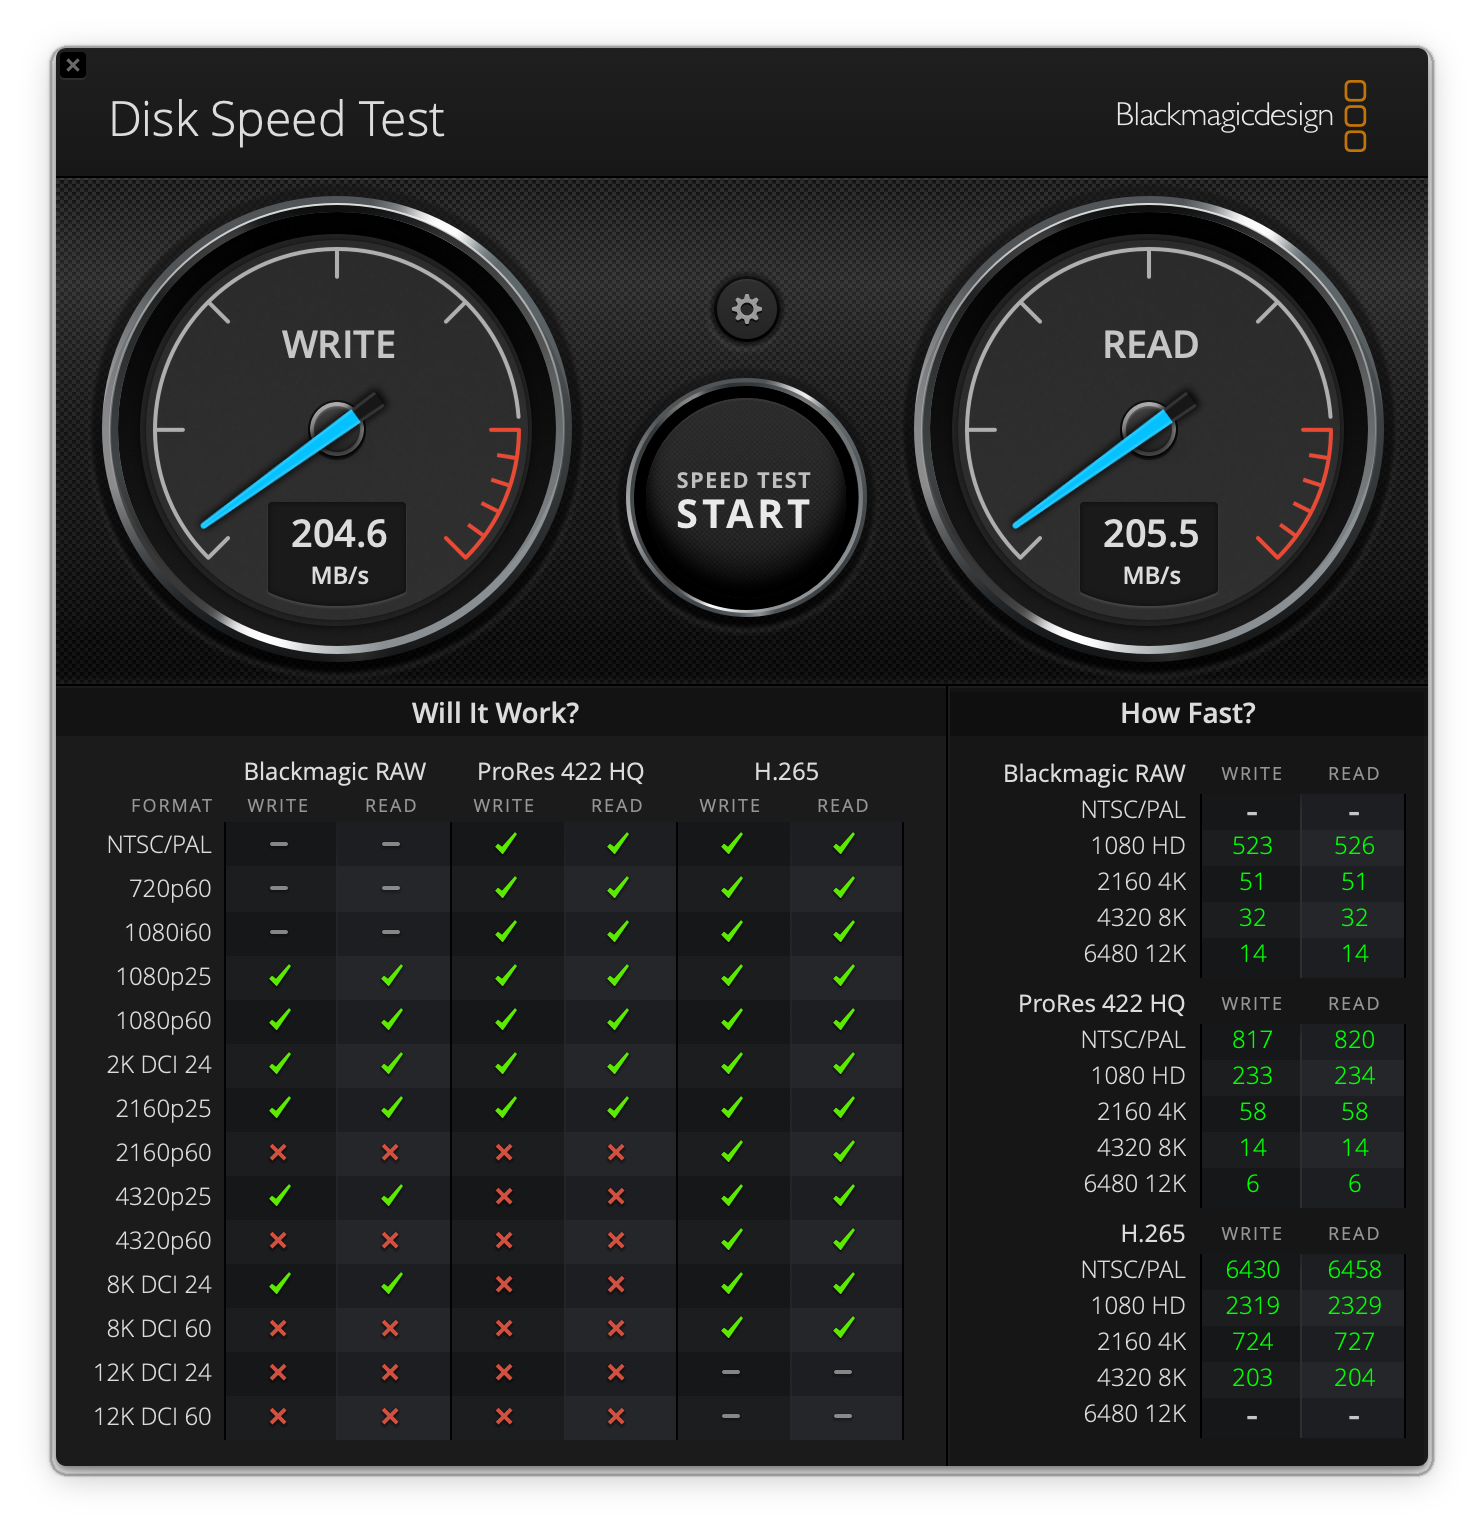
\includegraphics[width=\linewidth]{一块常见的2.5寸HHD盘.png}
        \caption{常见 2.5 寸混合硬盘 (HHD) 测速}
    \end{minipage}%
    \hfill%
    \begin{minipage}[t]{0.48\linewidth}
        \centering
        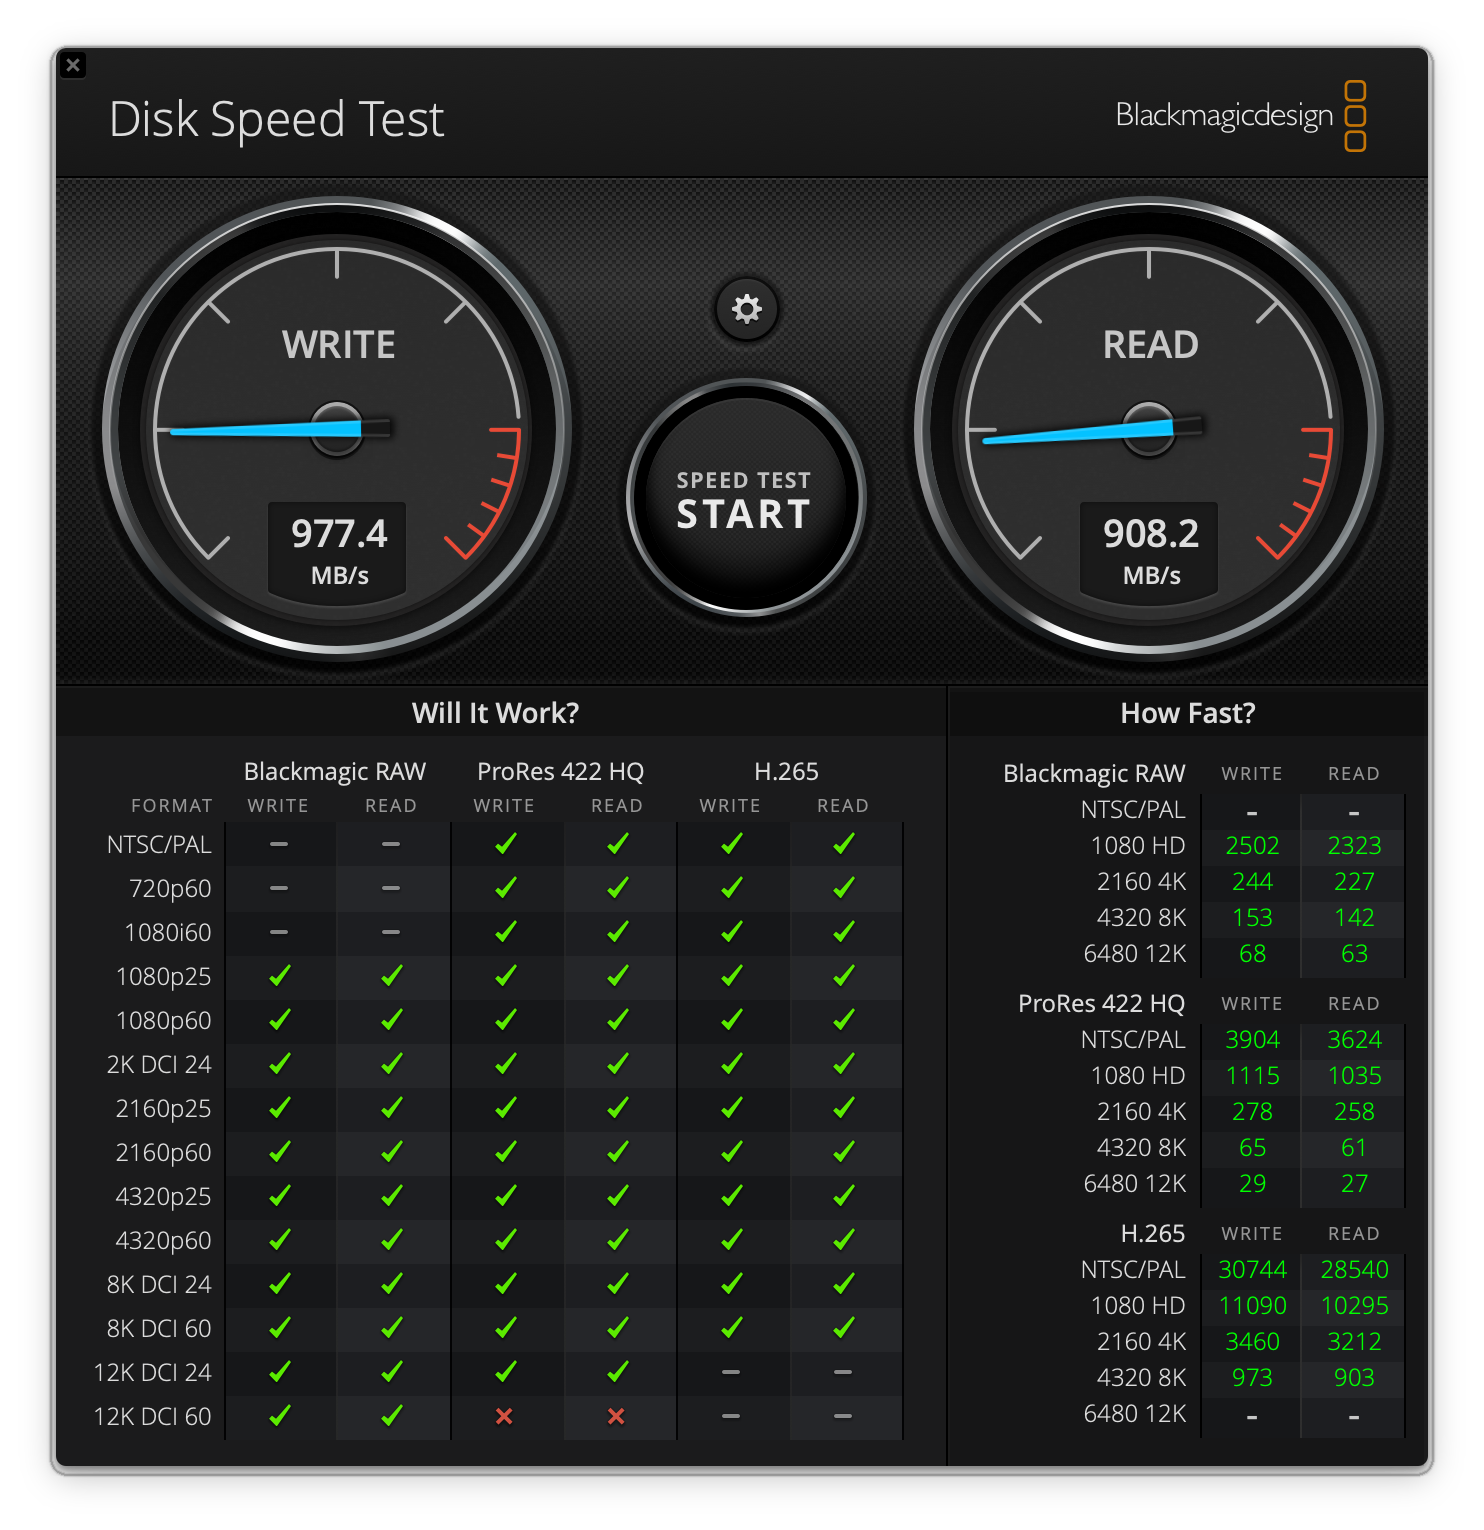
\includegraphics[width=\linewidth]{ssd.png}
        \caption{固态硬盘 (SSD) 测速，速度优势明显}
    \end{minipage}
\end{figure}

\begin{itemize}
    \item \textbf{格式化规则：} 根据后期剪辑的系统选择 APFS 或 NTFS。通常的原则是——\textbf{盘是谁的，或者导演用什么电脑，就把盘格式化成什么格式}。
\end{itemize}

\begin{figure}[H]
    \centering
    \begin{minipage}[t]{0.48\linewidth}
        \centering
        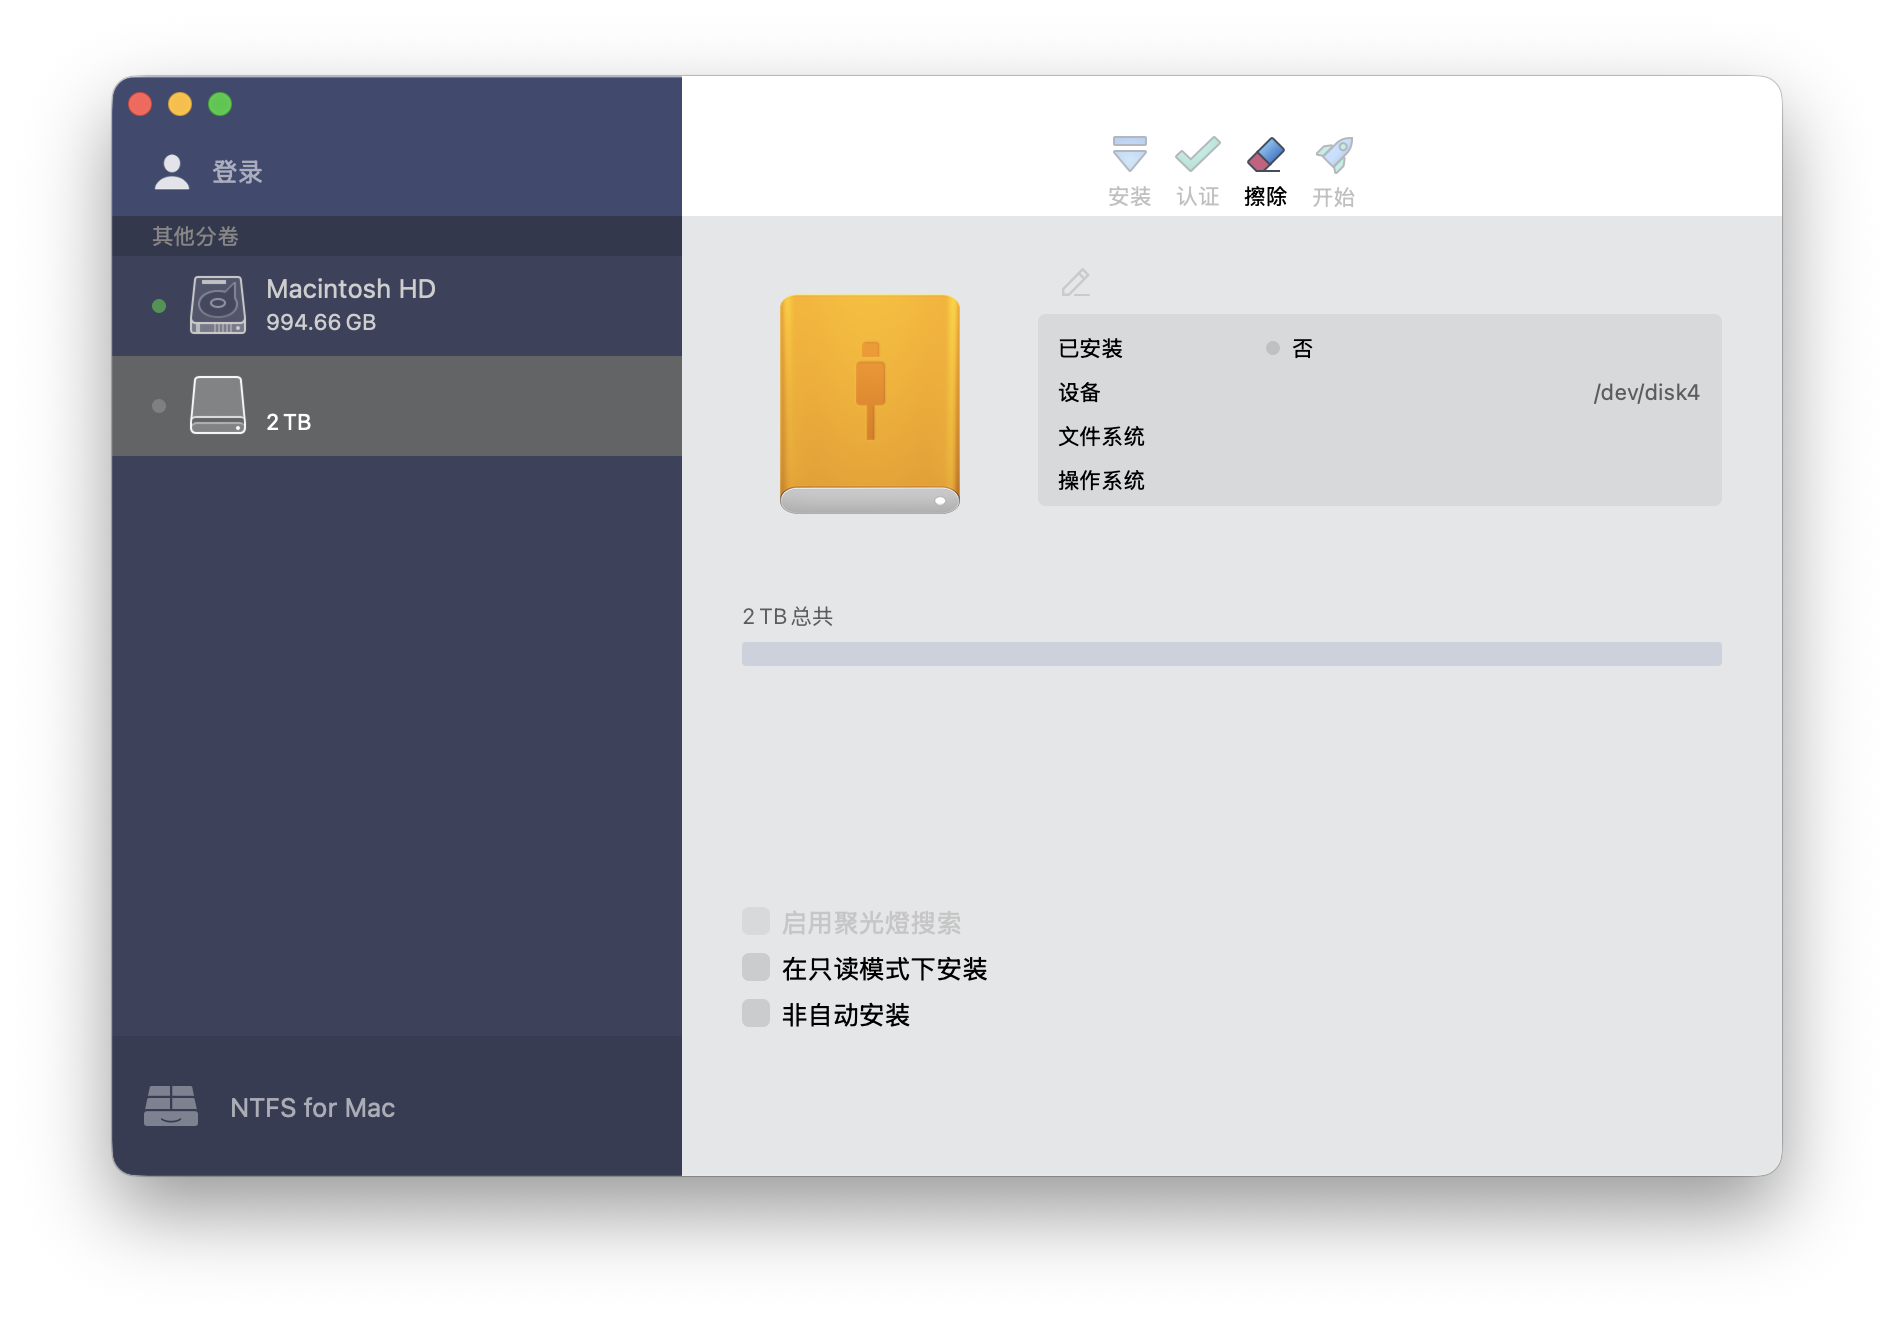
\includegraphics[width=\linewidth]{ntfs格式化1.png}
        \caption{打开NTFS for Mac并选择目标硬盘}
    \end{minipage}%
    \hfill%
    \begin{minipage}[t]{0.48\linewidth}
        \centering
        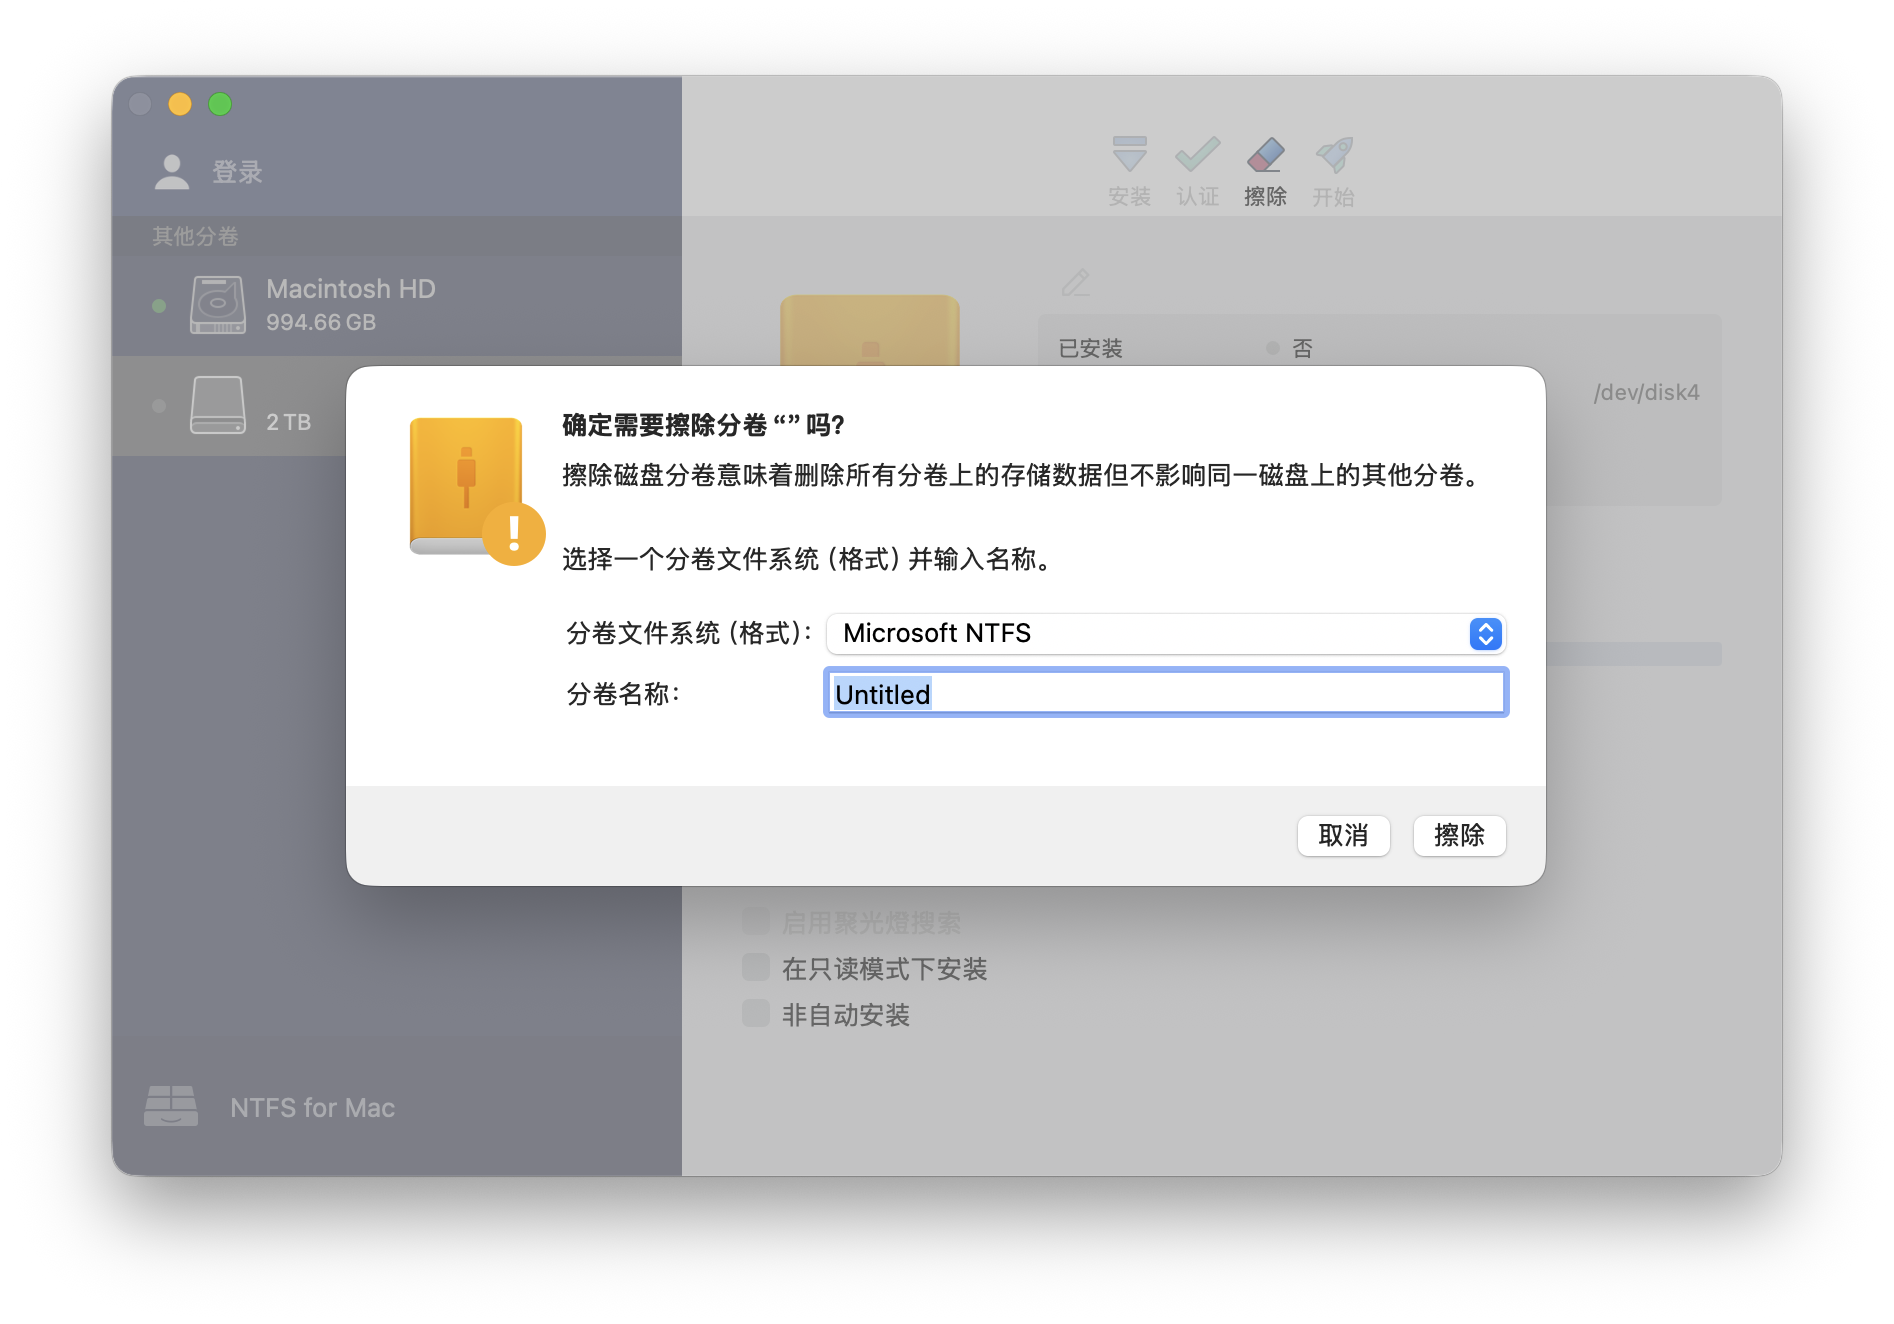
\includegraphics[width=\linewidth]{ntfs格式化2.png}
        \caption{点击擦除并选择 NTFS 的格式化}
    \end{minipage}
\end{figure}

在 NTFS for Mac 插件中，可以将硬盘格式化为 NTFS 格式（这对于后期在 Windows 平台上剪辑的剧组至关重要）。

\begin{figure}[H]
    \centering
    \begin{minipage}[t]{0.48\linewidth}
        \centering
        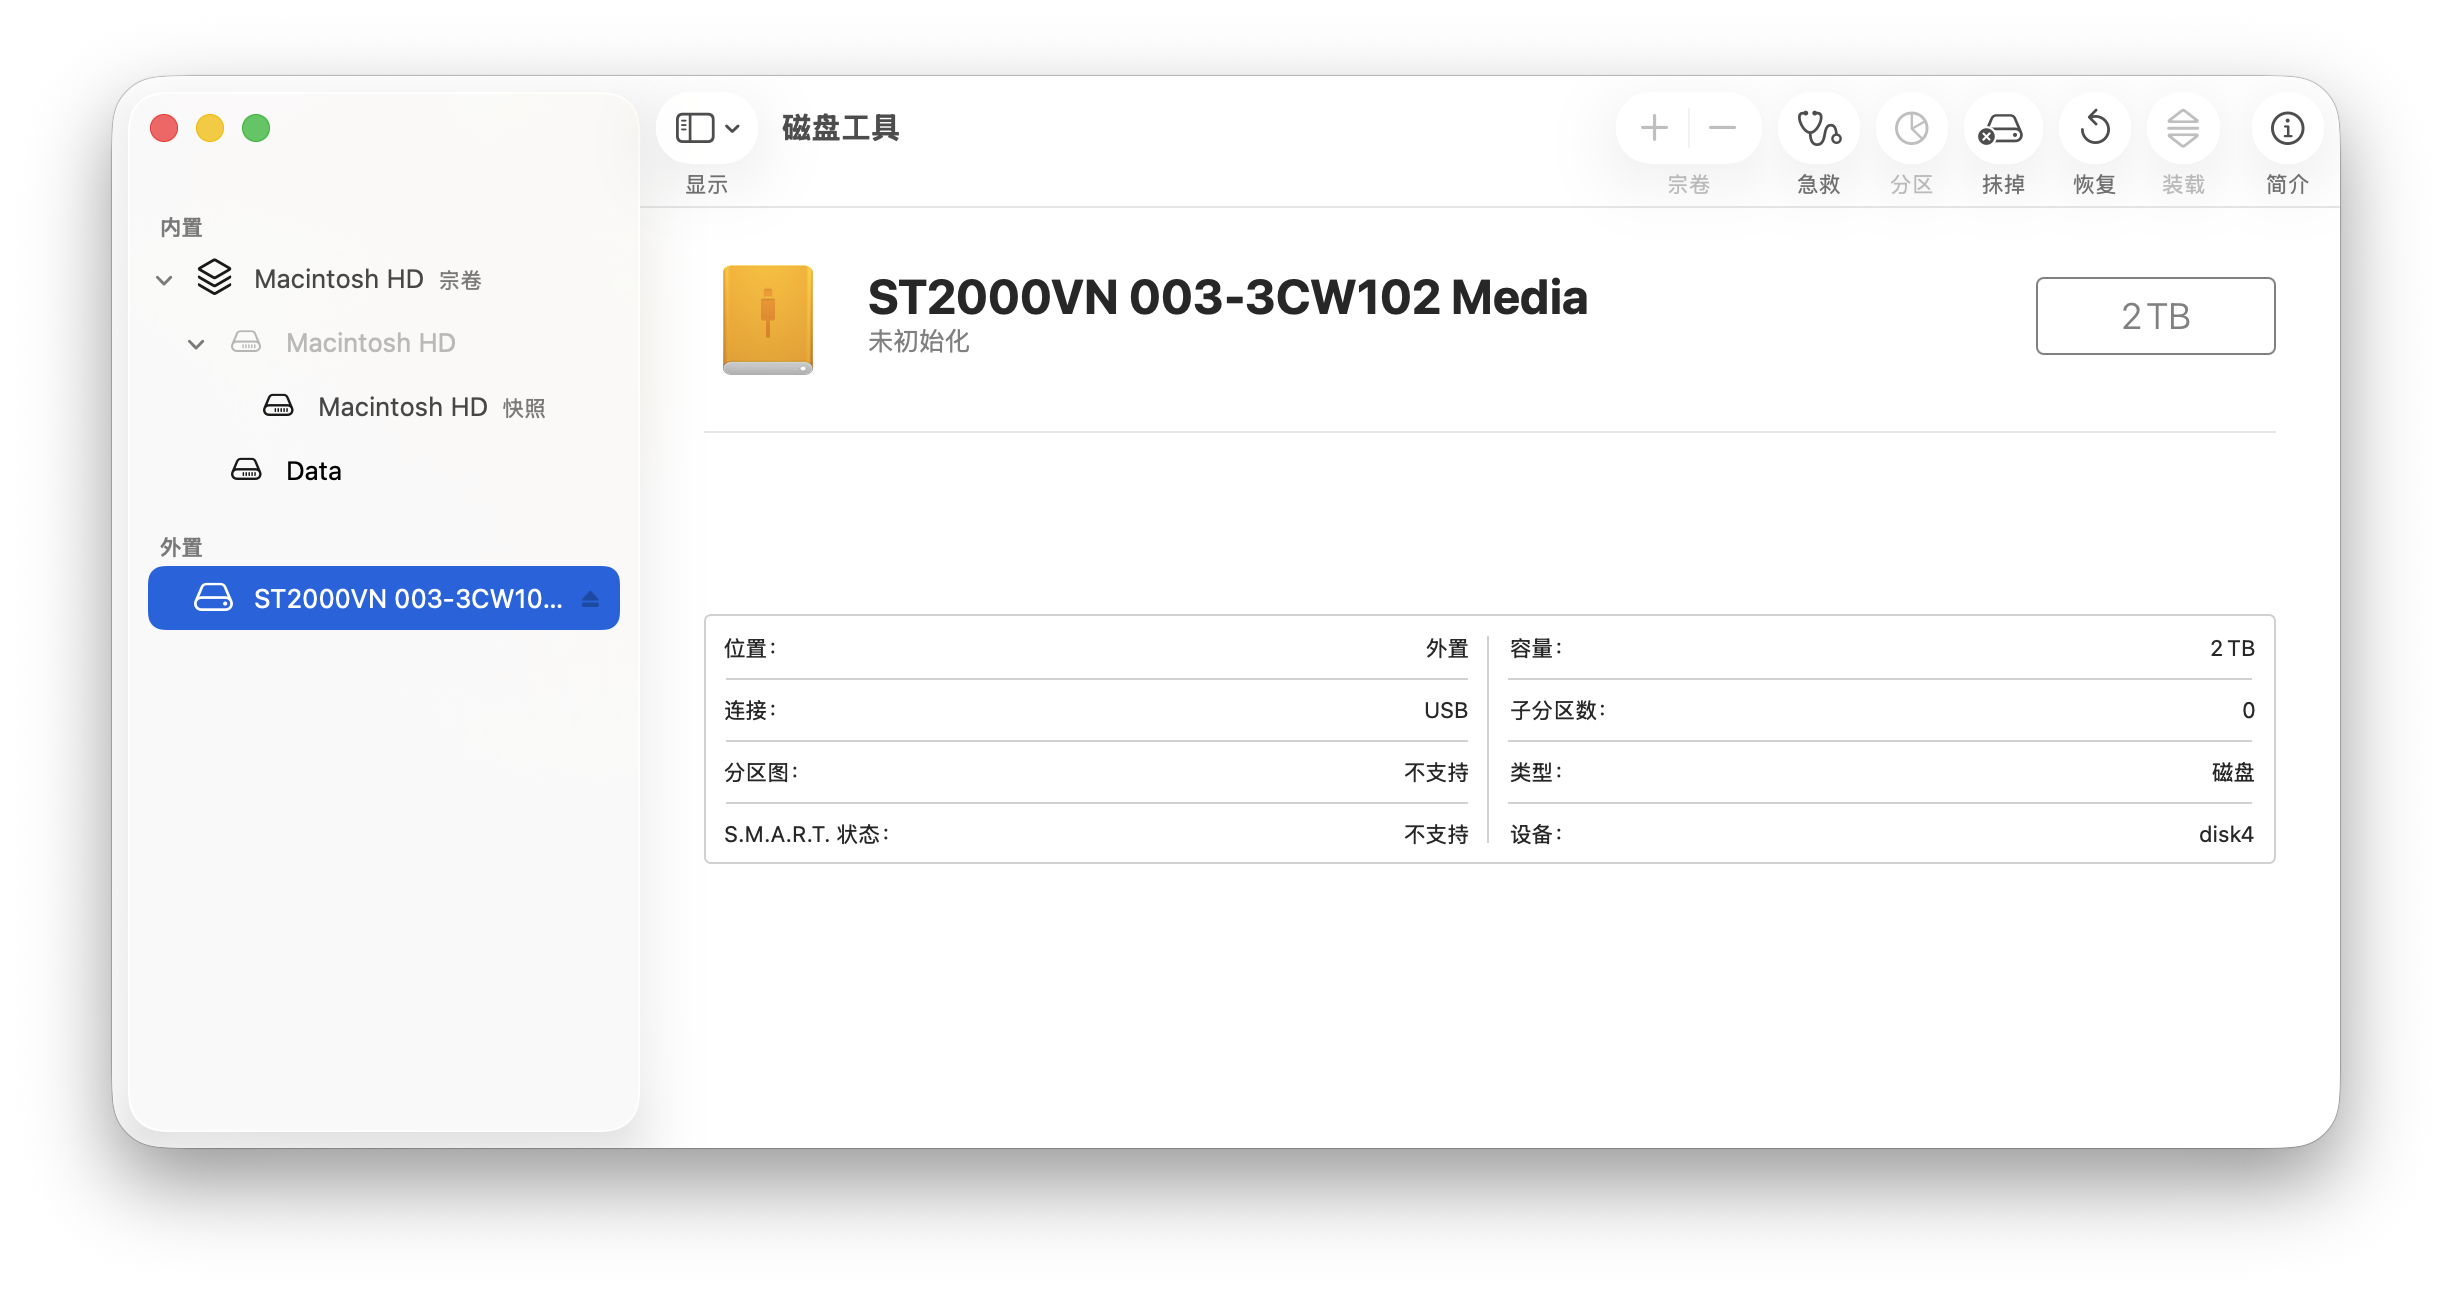
\includegraphics[width=\linewidth]{磁盘工具格式化1.png}
        \caption{部分盘即使无法读写，磁盘工具也可以看到连接状态}
    \end{minipage}%
    \hfill%
    \begin{minipage}[t]{0.48\linewidth}
        \centering
        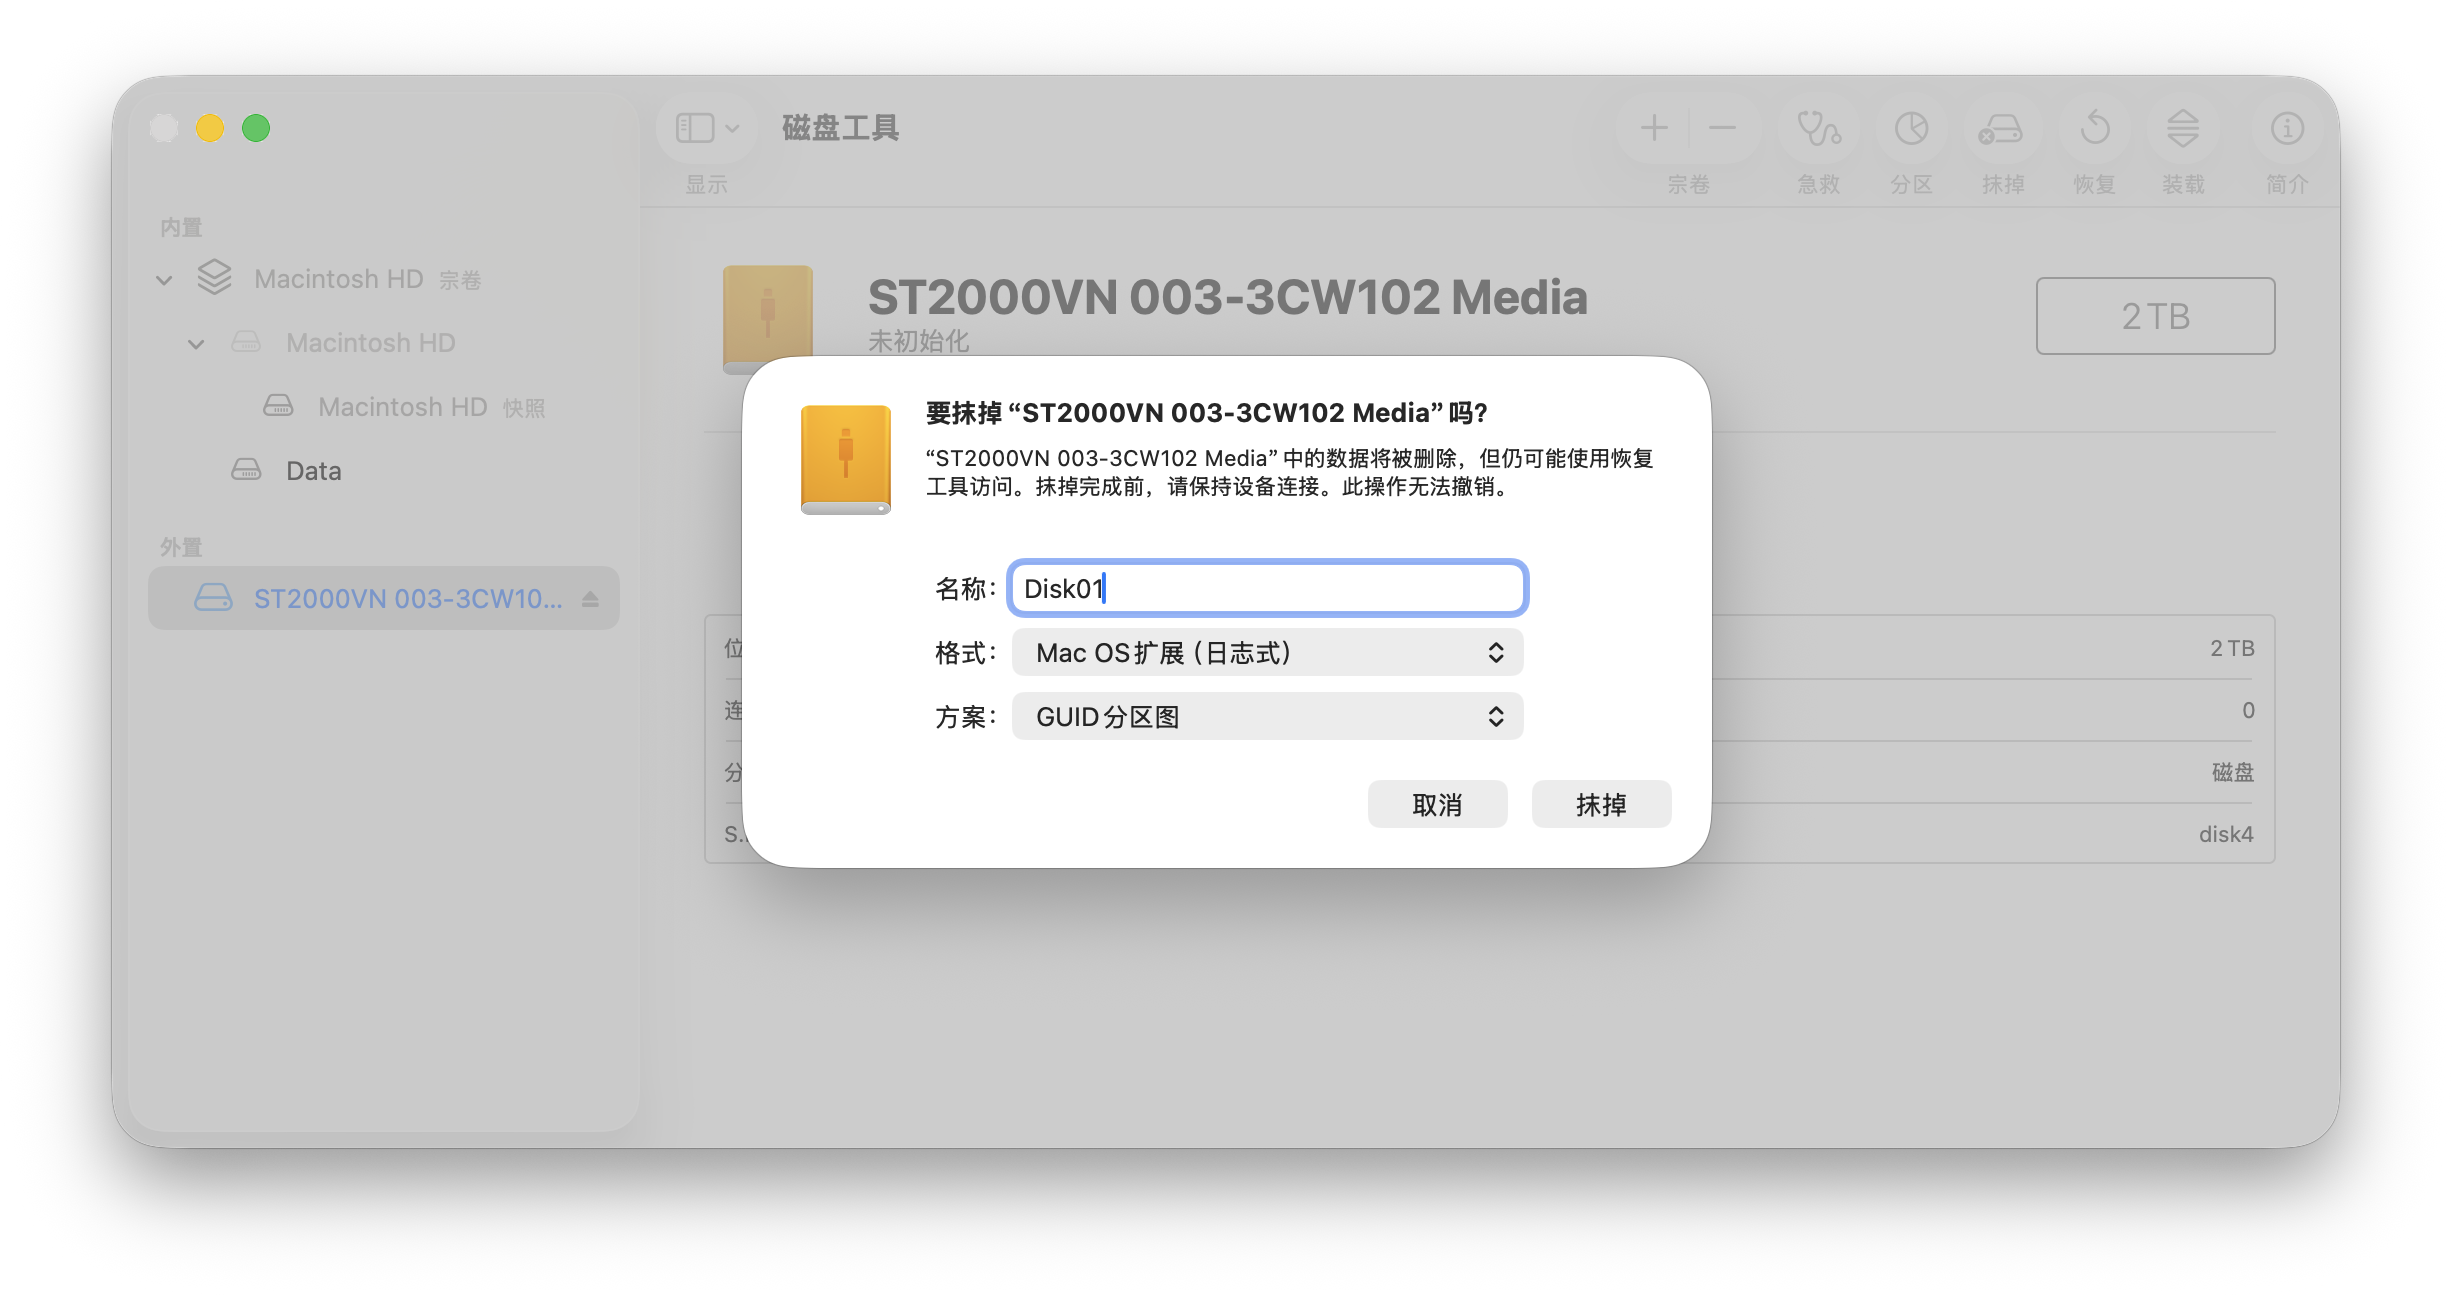
\includegraphics[width=\linewidth]{磁盘工具格式化2.png}
        \caption{选择需要的磁盘格式，进行格式化}
    \end{minipage}
\end{figure}

在 macOS 系统自带的“磁盘工具”中，可以格式化硬盘为 APFS。关于常见的磁盘格式，作为 DIT 必须牢记以下辨析：

\begin{tcolorbox}[colback=white, colframe=LineGrey, boxrule=0.5pt, arc=1mm, breakable]
\small
\textbf{【DIT 避坑必看】常见磁盘格式辨析：}
\begin{itemize}
    \item \textbf{APFS (Apple 文件系统)：} 苹果专为固态硬盘 (SSD) 优化的现代格式。速度极快，复制文件极度高效，安全性高。在使用磁盘工具格式化时，需要注意以下区分：
    \begin{itemize}
        \item \textbf{APFS：}使用 APFS 格式。如果不需要加密或区分大小写格式，请选取此选项。
        \item \textbf{APFS（加密）：}使用 APFS 格式且加密宗卷。
        \item \textbf{APFS（区分大小写）：}使用 APFS 格式并区分文件和文件夹名称的大小写。例如，名称为“Homework”和“HOMEWORK”的文件夹是两个不同的文件夹。
        \item \textbf{APFS（区分大小写，加密）：}使用 APFS 格式，区分文件和文件夹名称的大小写且加密宗卷。例如，名称为“Homework”和“HOMEWORK”的文件夹是两个不同的文件夹。
    \end{itemize}
    \textbf{建议：} 只要是 SSD 且后期全在 Mac 上做，\textbf{无脑选最基础的 APFS 即可}。
    
    \item \textbf{Mac OS 扩展 (日志式) / HFS+：} 苹果上一代经典格式，对传统的机械硬盘 (HDD) 架构更友好。\\ \textbf{建议：} 如果剧组给的备盘（Backup）是机械硬盘，建议格式化为日志式。
    
    \item \textbf{NTFS：} Windows 原生格式，非常稳定。缺点是 Mac 原生只能读不能写，必须依赖第三方插件。\\ \textbf{建议：} 如果后期明确使用 Windows 系统，主盘务必使用 NTFS。
    
    \item \textcolor{AlertRed}{\textbf{ExFAT (排雷警告！)：}} 这是一个看似能跨平台直接读写的美好陷阱，但它\textbf{没有日志记录功能}。在片场混乱的环境下，一旦供电中断或不小心踢掉数据线，整个分区极易损坏且数据难以恢复！\\ \textbf{建议：} \textbf{打死不用！}除非你用的是U盘。
\end{itemize}
\end{tcolorbox}


\subsection{开拍前的“逼问”}
\begin{itemize}
    \item \textbf{了解数据量与格式：} 问导演关于片长、预算等一些必要的细节，他们往往不会主动告诉你。有了这些才能预估数据量，提前规避碟中谍的任务（mission impossible）。同时要和 DP 商量最终的录制格式，比如是拍 ProRes 422 还是 ARRIRAW？RAW 的数据量极大，结合导演给的片长和预算，如果剧组只准备了两块 1T 硬盘却要拍 RAW，必须立刻要求制片组增加硬盘预算，否则很快就会面临没盘可用的绝境。如果只准备了一块1t盘并问你能不能做双备份，此时需要稳住血压进行解释，并考虑后续情况选择离开此组（划掉）。
    \item \textbf{器材确认：} 和 DP 商量具体器材。如果 DP 靠谱，相信他并做好自己的事，不是管得越多越好。
    \item \textbf{时码器核对：} 和出设备的人确认时码器出了没有。询问录音的设备很关键，录音设备导入时码所需的线材是 SDI 还是 3.5mm 不一定会随时码器一起出，必须提前准备好，不然没有时码后期剪辑会吐血。
\end{itemize}


\newpage
% ==========================================
% 第三章 数据与媒体管理
% ==========================================
\section{数据与媒体管理 (Data \& Media Management)}
\label{sec:data_management}

在这个阶段，我们将使用行业标准软件 \textbf{Silverstack Lab}。它的核心价值在于校验 Checksum。直接拖拽复制是对心血的不负责任，除非你是某系的学生。

\subsection{前期预建与项目设置}
\textbf{1. 建立硬盘结构：} 在主盘和备盘里建好空文件夹。
推荐结构如下：
\begin{tcolorbox}[colback=white, colframe=TextGrey, boxrule=0.5pt, sharp corners]
\small\ttfamily
/Day\#\#\#\_\#\#\#\#\#\#\#\#\\
|-- 01\_Raw\\
|-- 02\_Sound\\
|-- 03\_ShotMetadata\\
|\ \ |-- EditList\\
|\ \ |-- QtakeALE\\
|\ \ |-- SilverstackCsv\\
|\ \ |-- SoundList\\
|\ \ |-- Thumbnail\\
|\ \ |-- ViewTransforms\\
|-- 04\_Transcode\\
|-- 05\_ProjectLibrary\\
|-- 06\_Report\\
|-- 07\_Stills\\
|-- 08\_Native
\end{tcolorbox}
\begin{figure}[H]
    \centering
    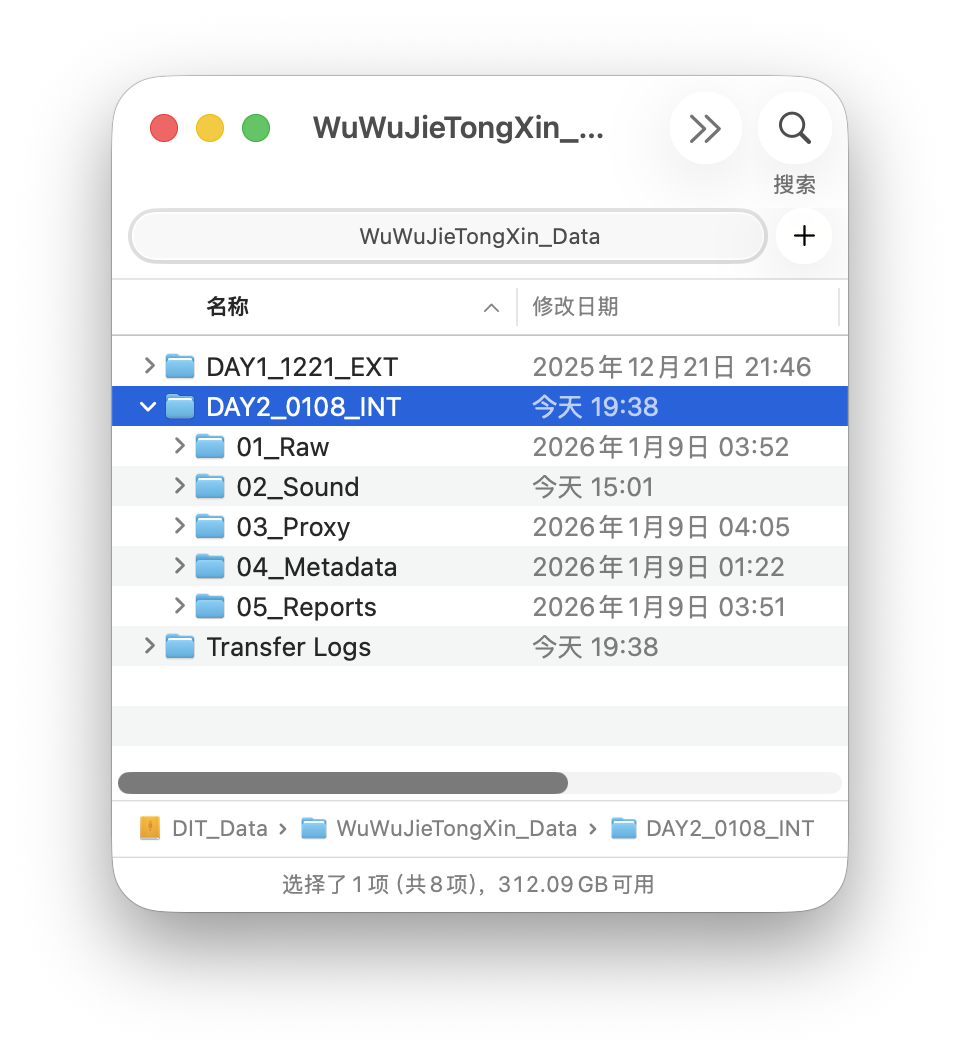
\includegraphics[width=0.9\linewidth]{文件夹结构.png}
    \caption{如果是学生剧组小型文件量，可以参考我这种结构}
\end{figure}

\textbf{2. 充电与设备清点：} 充满电脑和手机的电。拿到并收好所有盘和卡。确保时码都连好接上。如果不熟，可以直接搜索“品牌名+教程”，例如“谛听时码器配对”，下载 App 连上即可。

\textbf{3. 摄影机参数与监视器 Check：}
由于现实中摄影机十分不同，这里给出一些基本的需要特别注意的参数：
\begin{itemize}
    \item \textbf{录制格式与分辨率：} 再次确认是否与前期规划一致，严防误开低画质。
    \item \textbf{项目帧率与传感器帧率：} 升格拍摄时极易翻车！确保项目帧率（Project Rate）是正常帧率（如 25fps），仅调整传感器帧率（Sensor FPS），否则后期声画绝对无法同步。
    \item \textbf{色彩空间：} 坚决避免在机内烧录 Rec.709，确保输出的是正确的 Log 曲线（如 ARRI LogC 或 Sony S-Log3），为后期保留宽容度。
\end{itemize}
然后就是设置监视器，一般来说学生剧组的摄影组会连接好图传和大小监，但你还是需要去确认一下 SDI 接口位置，便于发现问题以及熟悉后续如果要加上 QTake 的操作。在简单的学生剧组中，确保导演看到的不是灰片，在监视器上选择摄影机拍摄格式对应的 LUT 即可。

\textbf{4. 创建项目与预填信息：} 打开软件选择 File -> New Project，输入项目名。调整常用布局方便查看元数据，提前填好导演、片名等固定信息。
\begin{figure}[H]
    \centering
    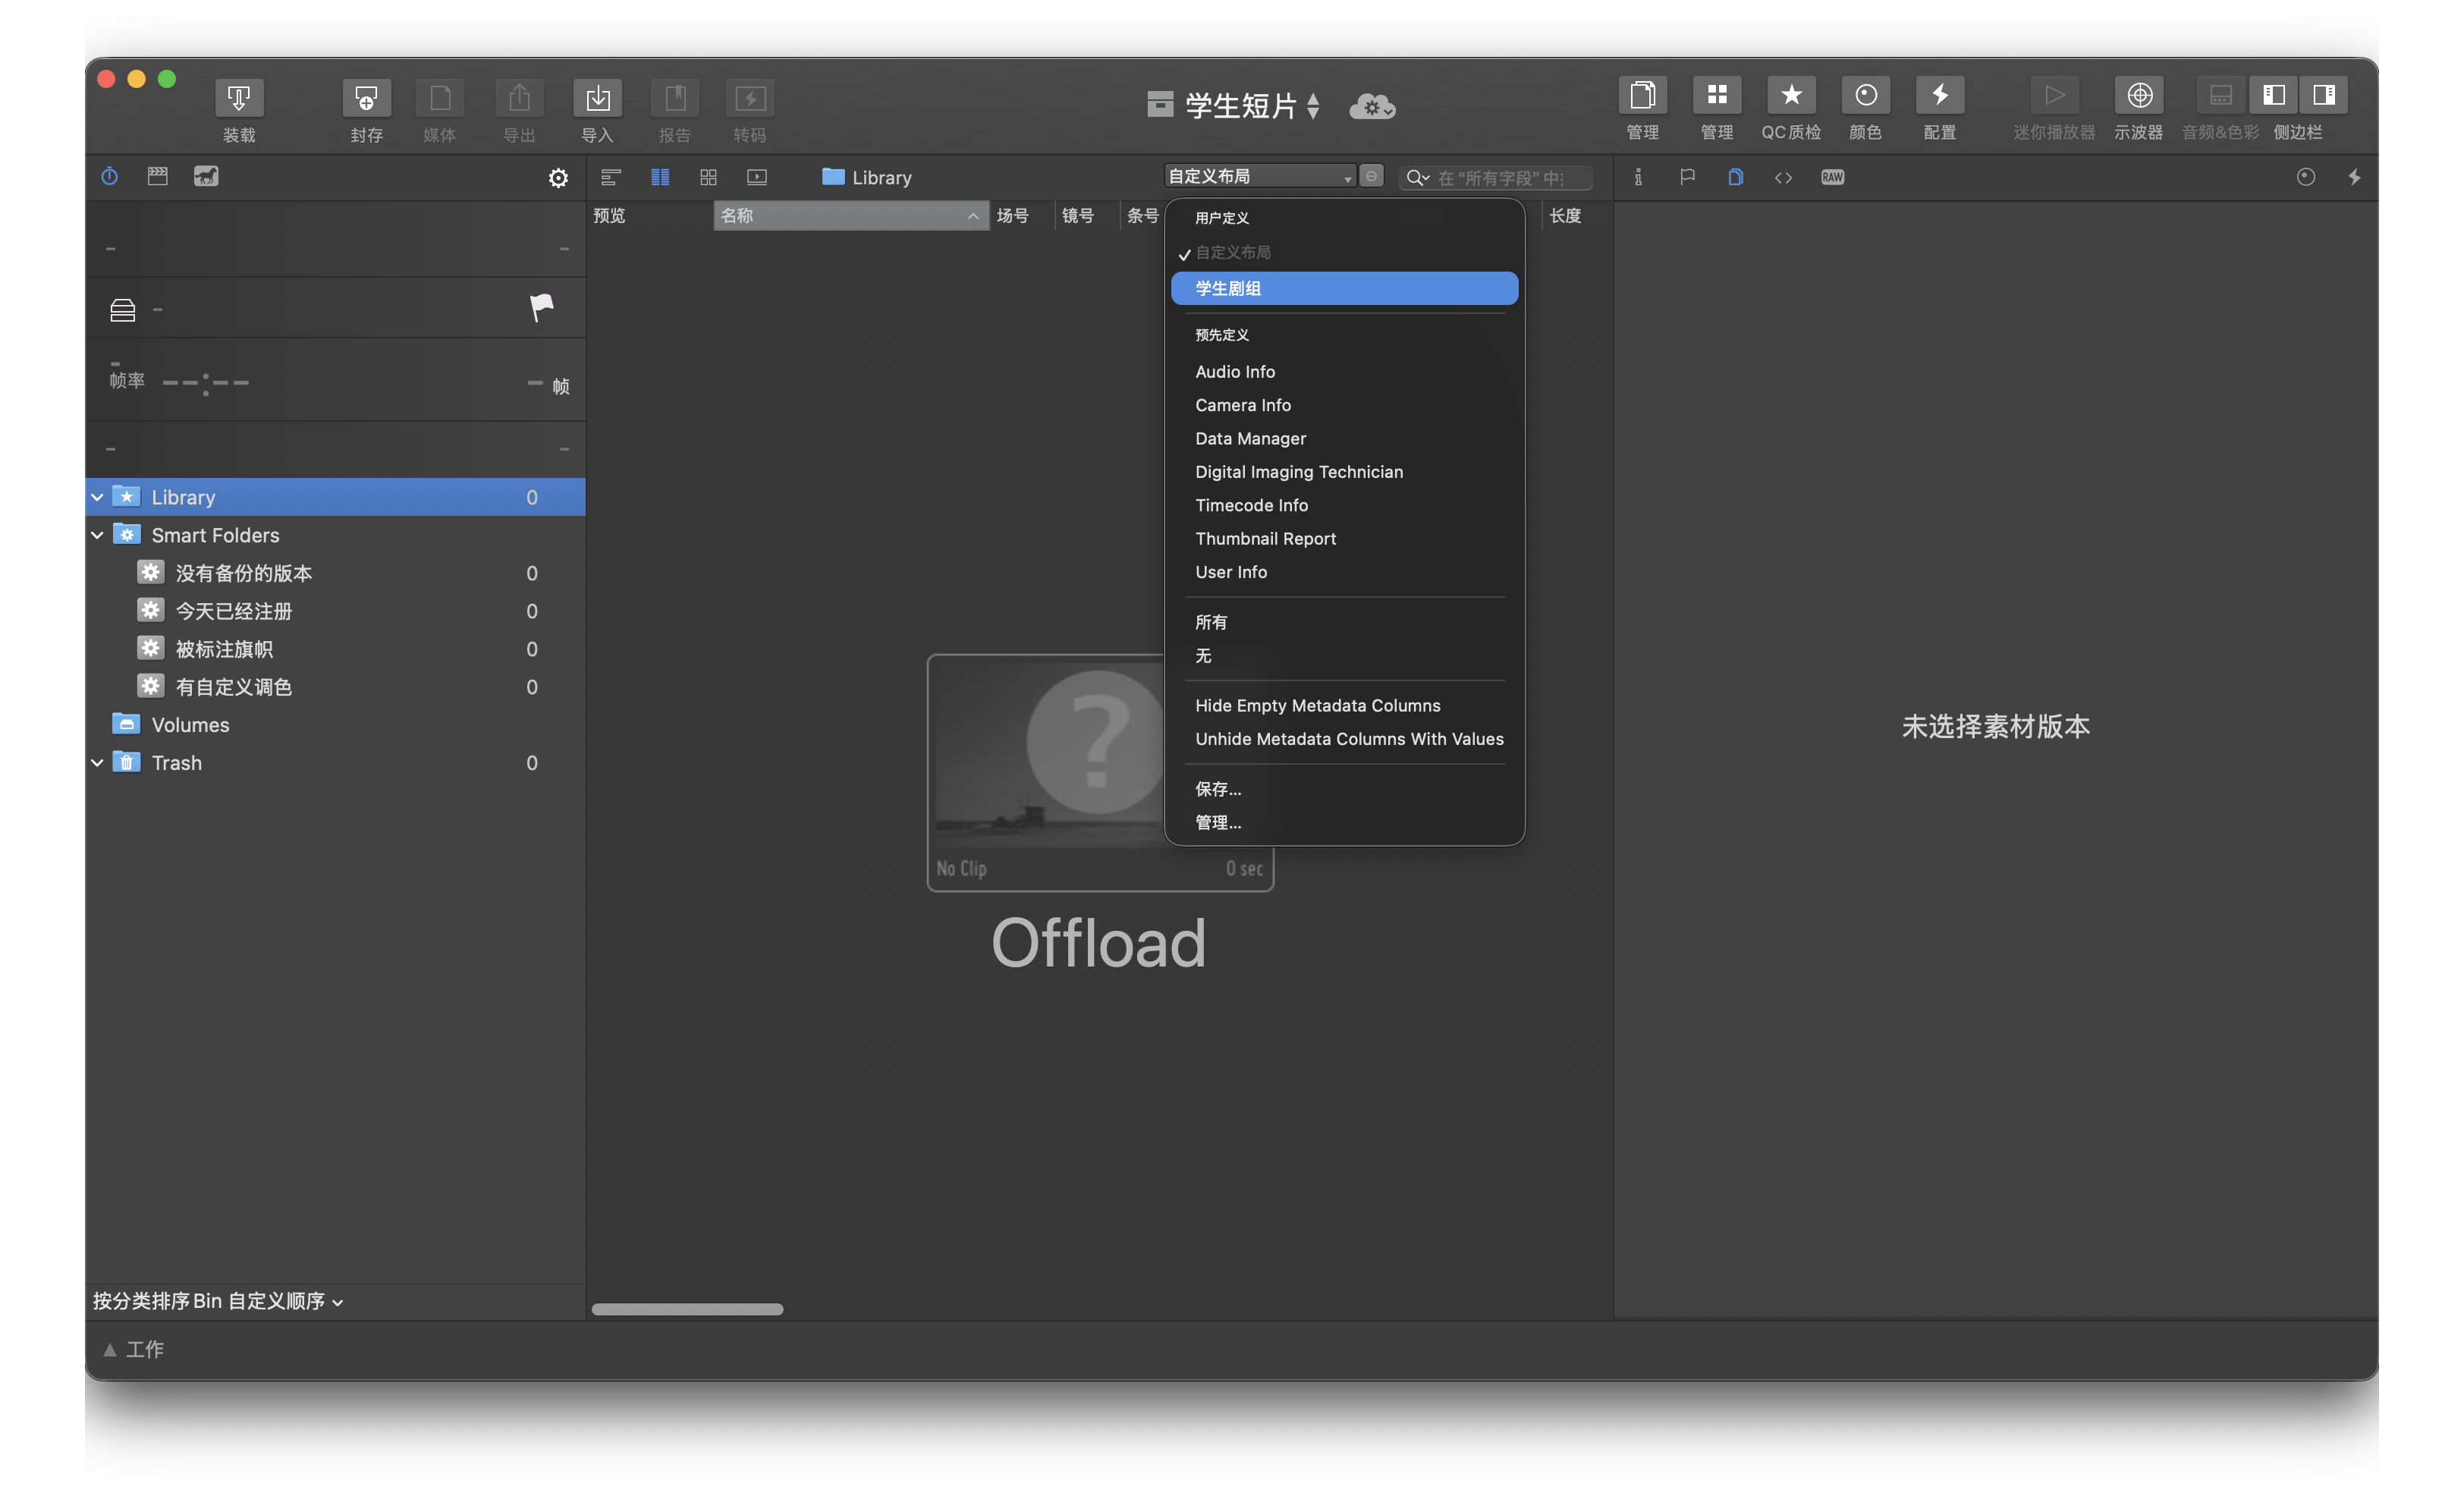
\includegraphics[width=0.85\linewidth]{布局修改.png}
    \caption{调整布局并预先填写项目名等数据}
\end{figure}

\subsection{现场安全拷卡 (Offload)}
第一张卡拍满后，亲手接过，用大力胶贴好读写口。把空卡交给摄影助理。插卡后，点击顶部的“装载”按钮。
\begin{itemize}
    \item \textbf{来源 Source：} 选存储卡。
    \item \textbf{目的地 Destinations：} 添加主盘和备盘两个路径，软件会同时向两块硬盘写入，效率最高。
    \item \textbf{文件夹结构：} 选 \texttt{Subfolder for each device}。我个人推荐在你不熟练的情况下先在外部建好文件夹，再拷贝进特定文件夹，特别是你没有提前拿到硬盘的时候。
    \item \textbf{校验 Verification：} 这是最重要的一步。Checksum 选 \texttt{xxHash64 (BE)} 以保证速度，或选 \texttt{MD5}。Behavior 选 \texttt{Verify Source \& Destination}。
    \item 点击 \texttt{Start Offload}。
    \begin{figure}[H]
        \centering
        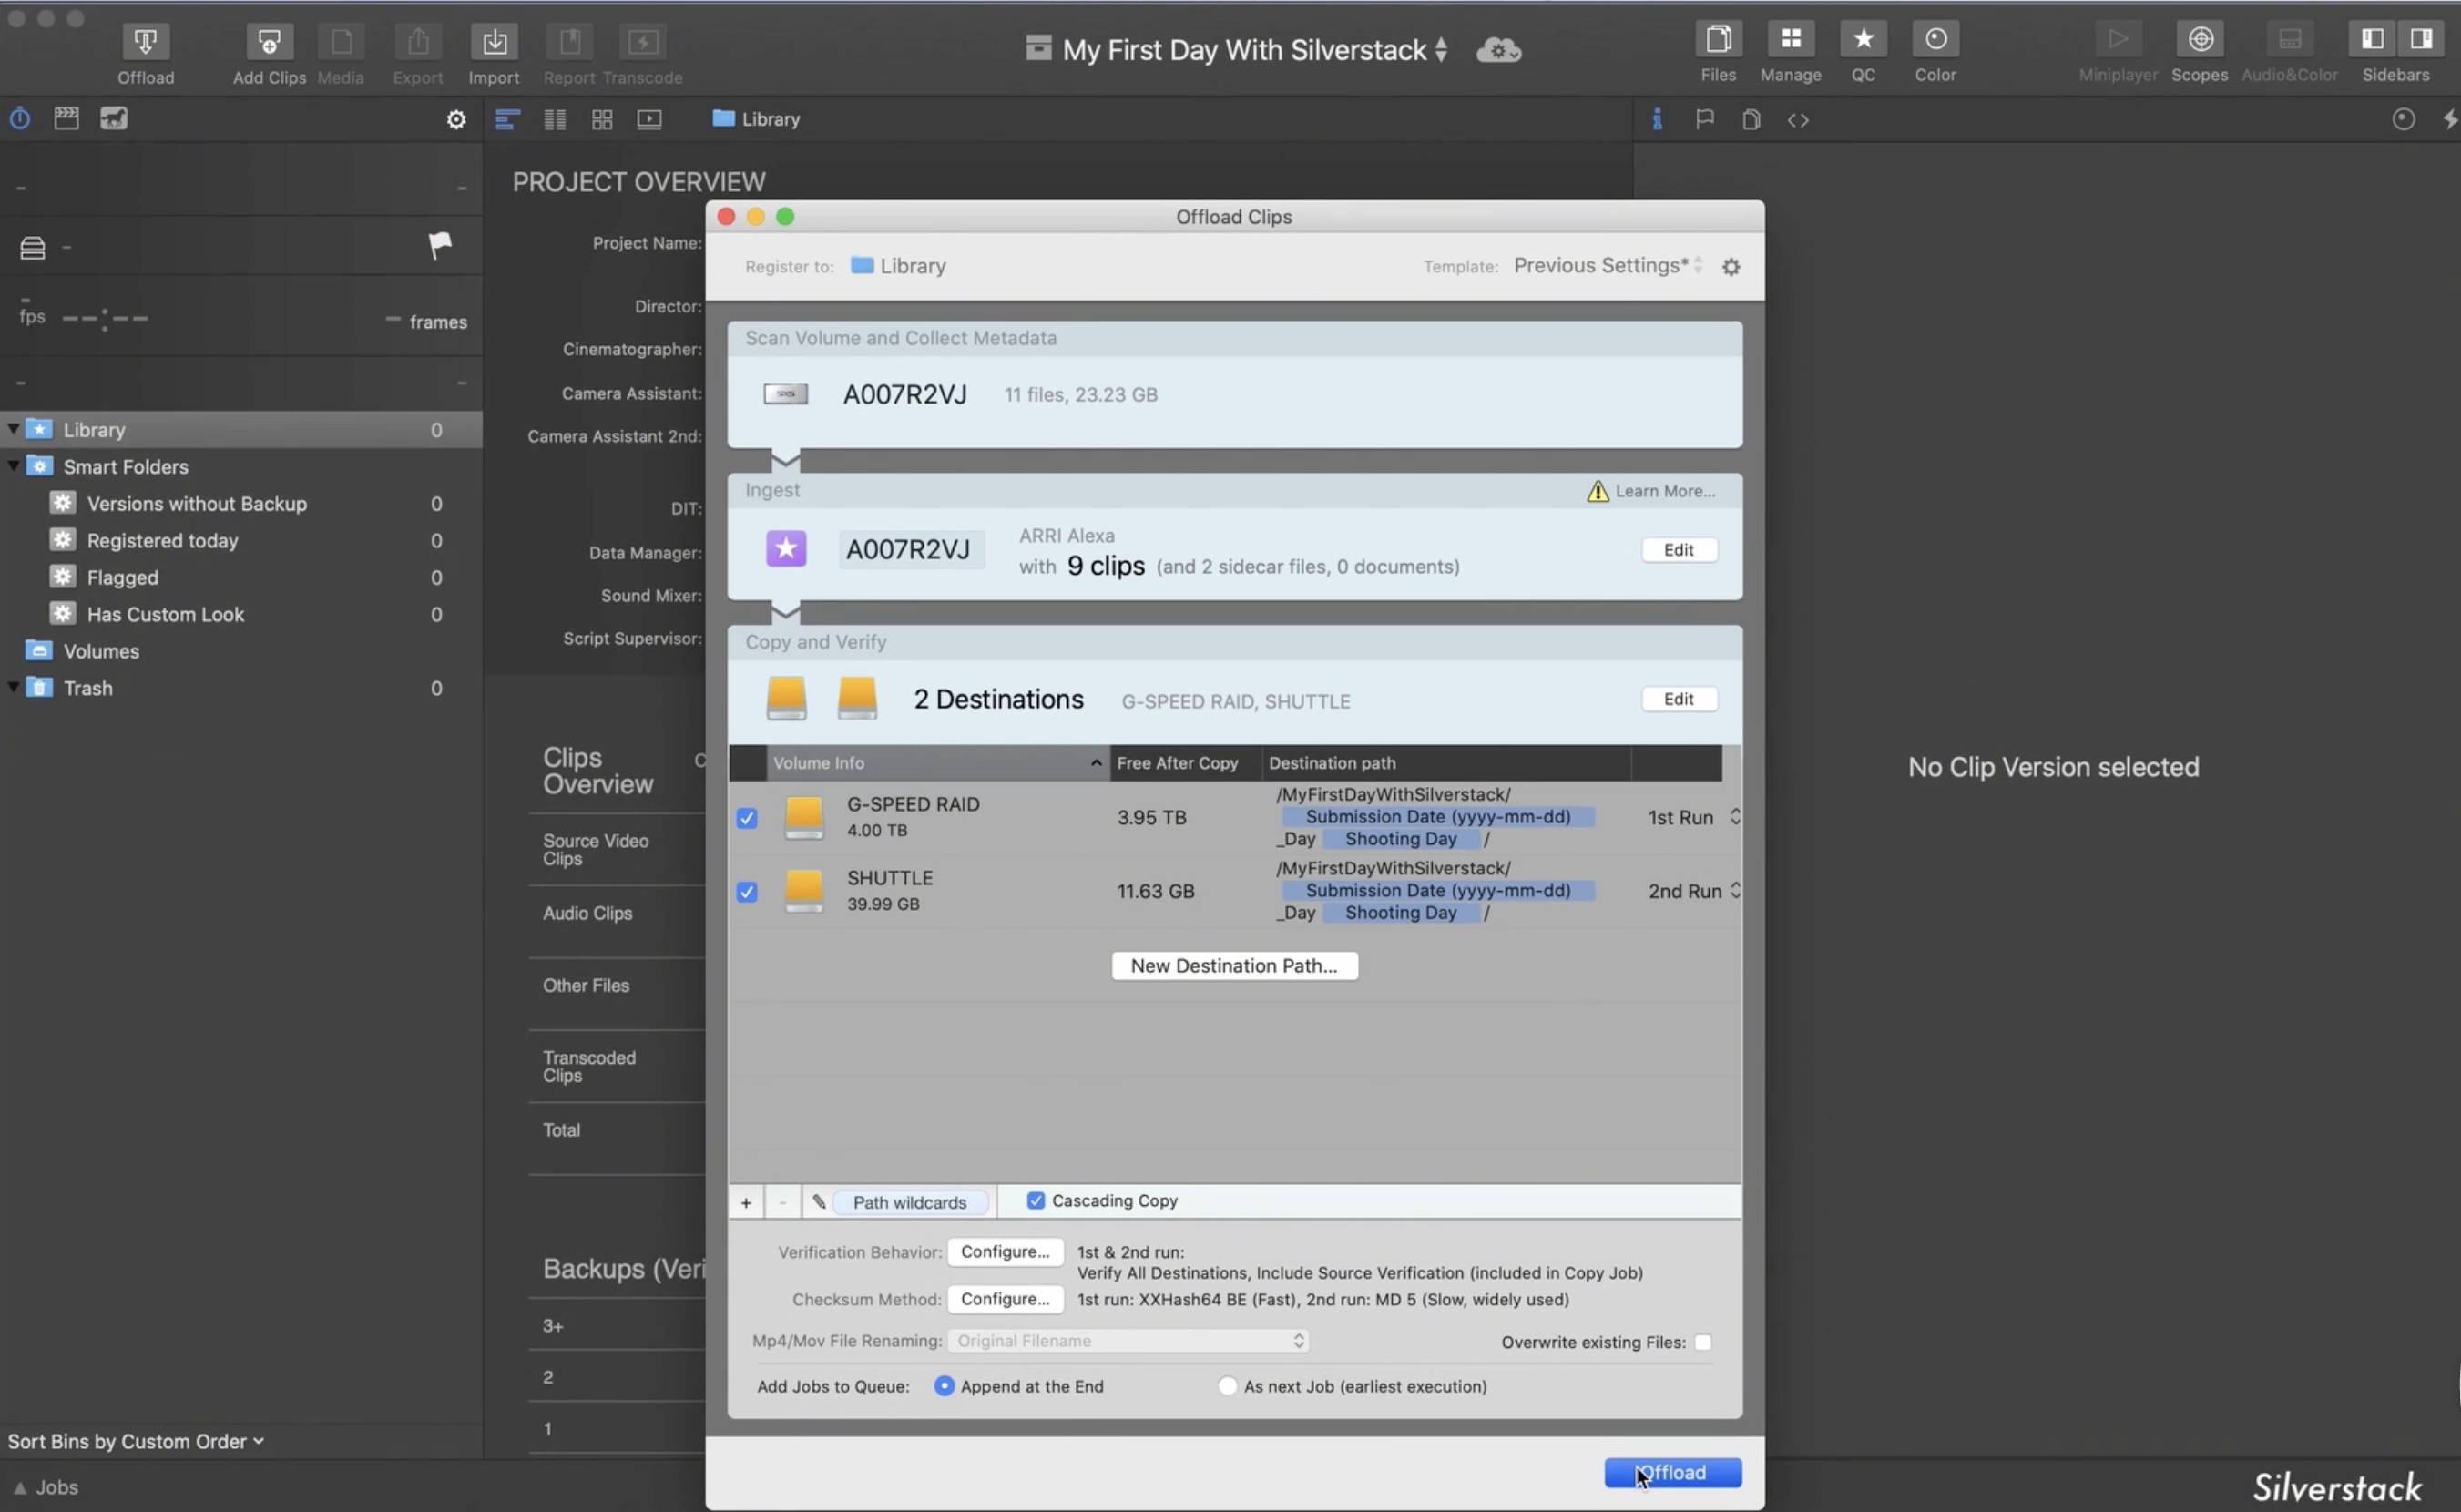
\includegraphics[width=1\linewidth]{下卡.png}
        \caption{拷卡界面设置}
    \end{figure}
    \item 基本上看中文翻译都可以直接操作。\\ \textbf{关于传递式拷贝 (Cascading Copy)：} 当你的拓展坞带宽不足以同时满速写入两块硬盘，或者主盘速度差异极大时（比如主盘是 SSD，备盘是慢速 HDD），可以开启此功能。软件会先将素材全速单线拷贝到最快的主盘并进行校验，然后再由主盘在后台自动复制到备盘。这样能以最快速度把读卡器解放出来。
\end{itemize}
观察进度条，绿色对钩代表成功，红色叉号代表报错（可能是线松了、盘满了或卡坏了），软件支持断点重续。


\newpage
% ==========================================
% 第四章 质量控制与元数据
% ==========================================
\section{质量控制与元数据 (QC \& Metadata)}
\label{sec:qc_metadata}

在安全拷卡的同时，DIT 需要对素材进行技术检查并整理核心元数据，为后期流程打好基础。

\subsection{预设“过、保、废”标签}
\textbf{\textcolor{WarningYellow}{\faLightbulb} 核心准备：提前预设“过、保、废”标签} \\
在开机前夜或开始干活前，强烈建议在 Silverstack 的项目设置中，自定义好标签（Labels）的名称与颜色（我个人习惯将其修改为直观的“过”、“废”、“保”、“空镜”等）。这些颜色之后会无缝转换为达芬奇中的“片段颜色（Clip Color）”，极大提升后期效率。
\begin{figure}[H]
    \centering
    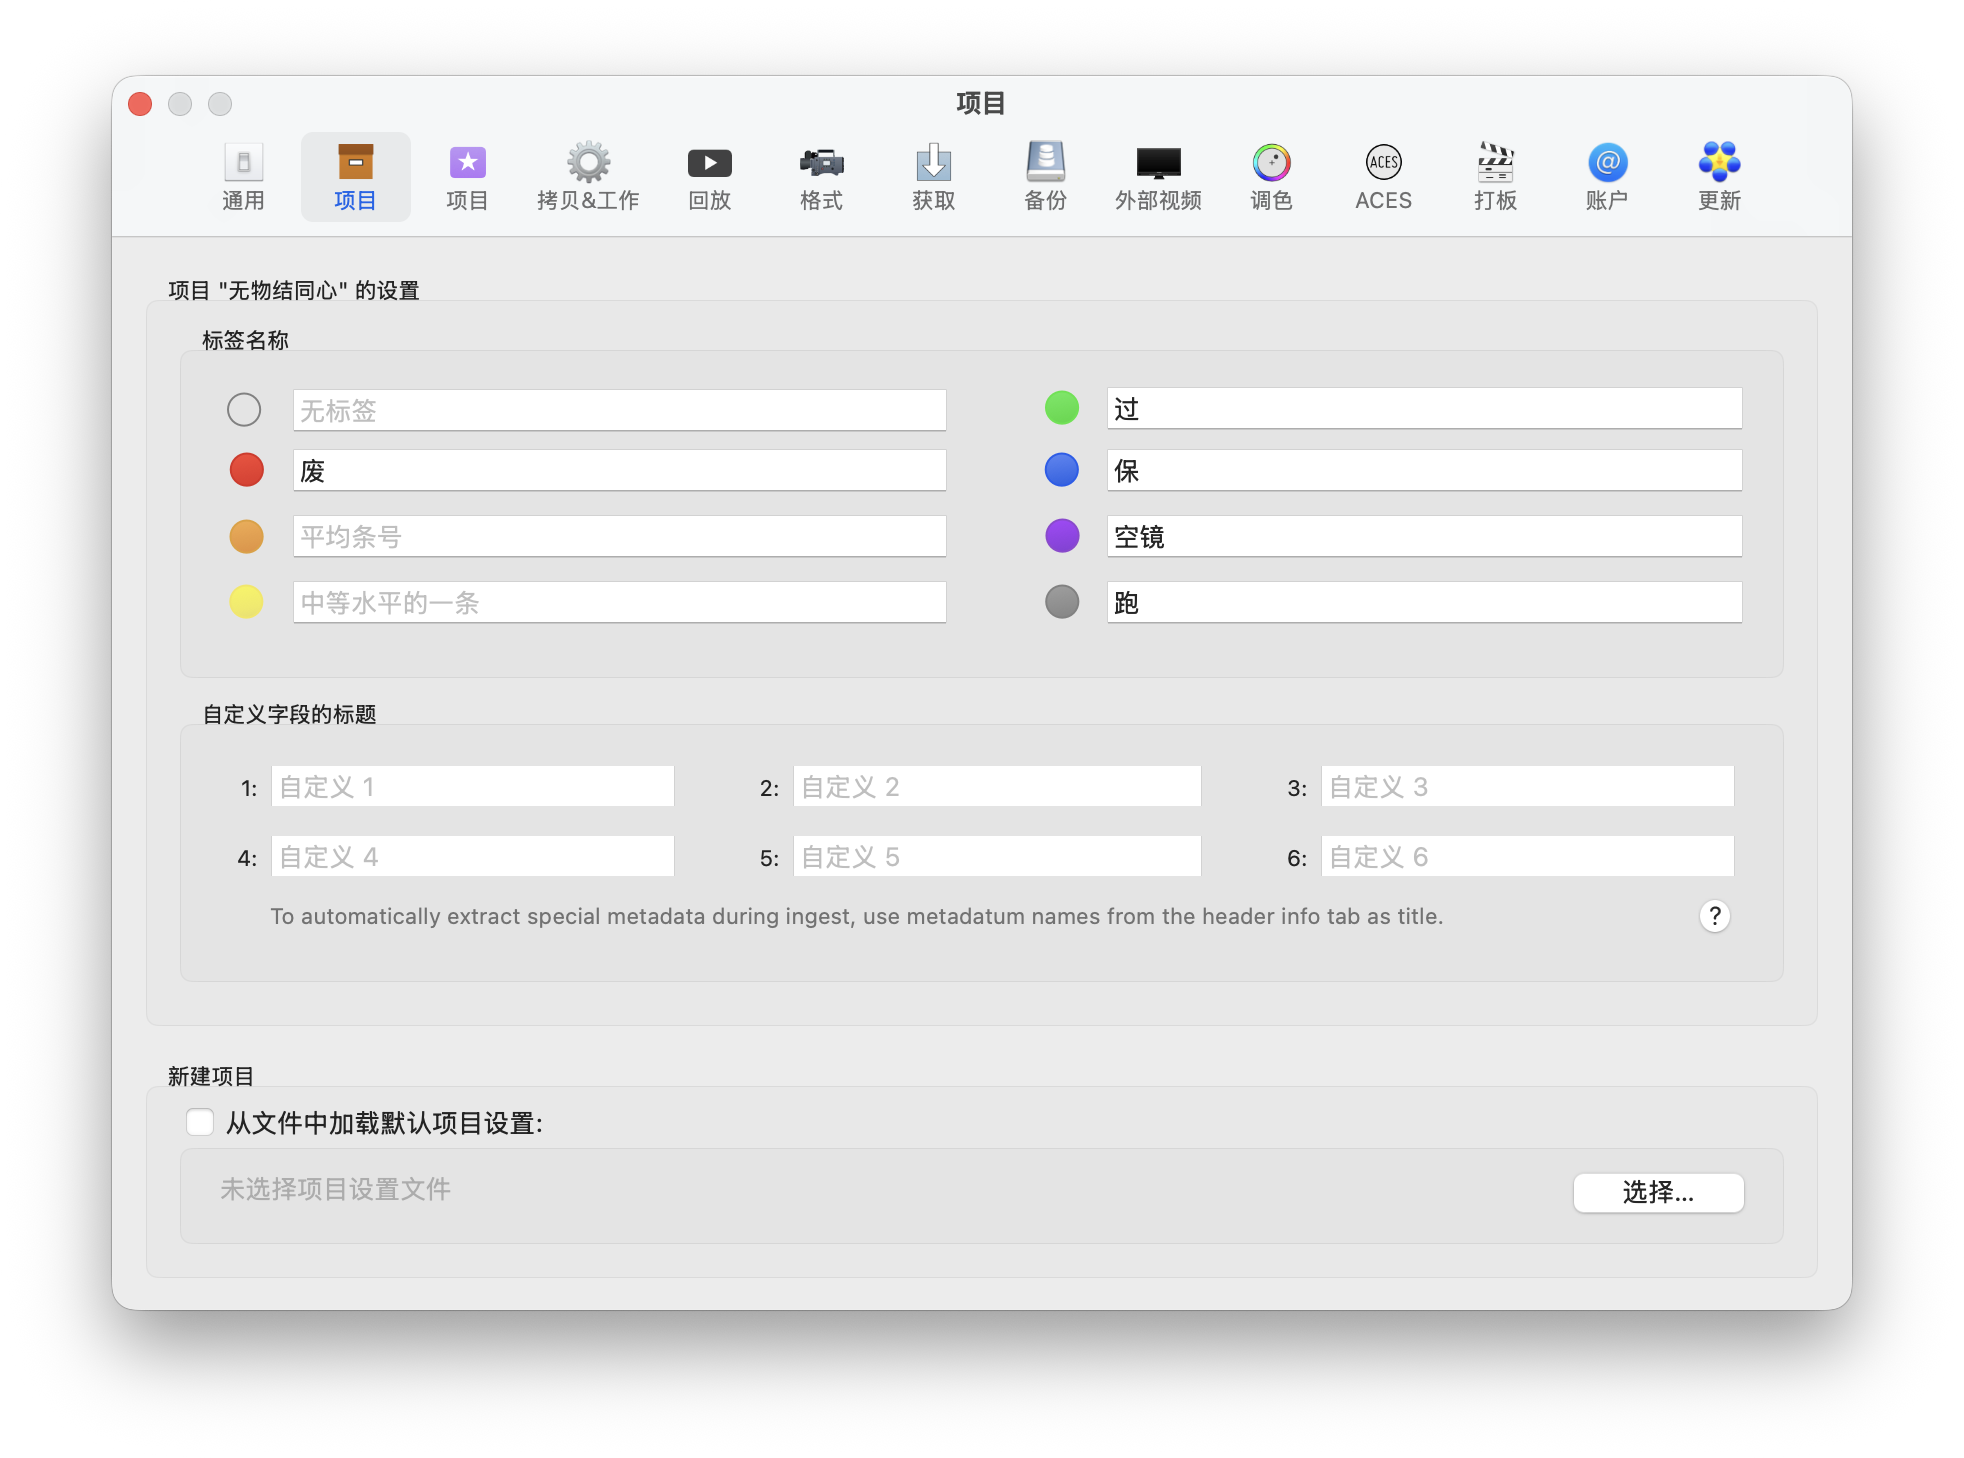
\includegraphics[width=0.85\linewidth]{标签颜色可以修改，我习惯改成这样的过报废.png} 
    \caption{在项目设置中自定义“过保废”标签与颜色}
\end{figure}

\subsection{打场镜次与 QC 质检}
拷卡期间向场记要场记单。点击软件顶部的“QC质检”星标，并在界面左上角切换为“列表视图（List View）”。在这里，你可以极其高效地给每一条素材填入场、镜、次信息，并打上对应的“过、保、废”标签。
\begin{figure}[H]
    \centering
    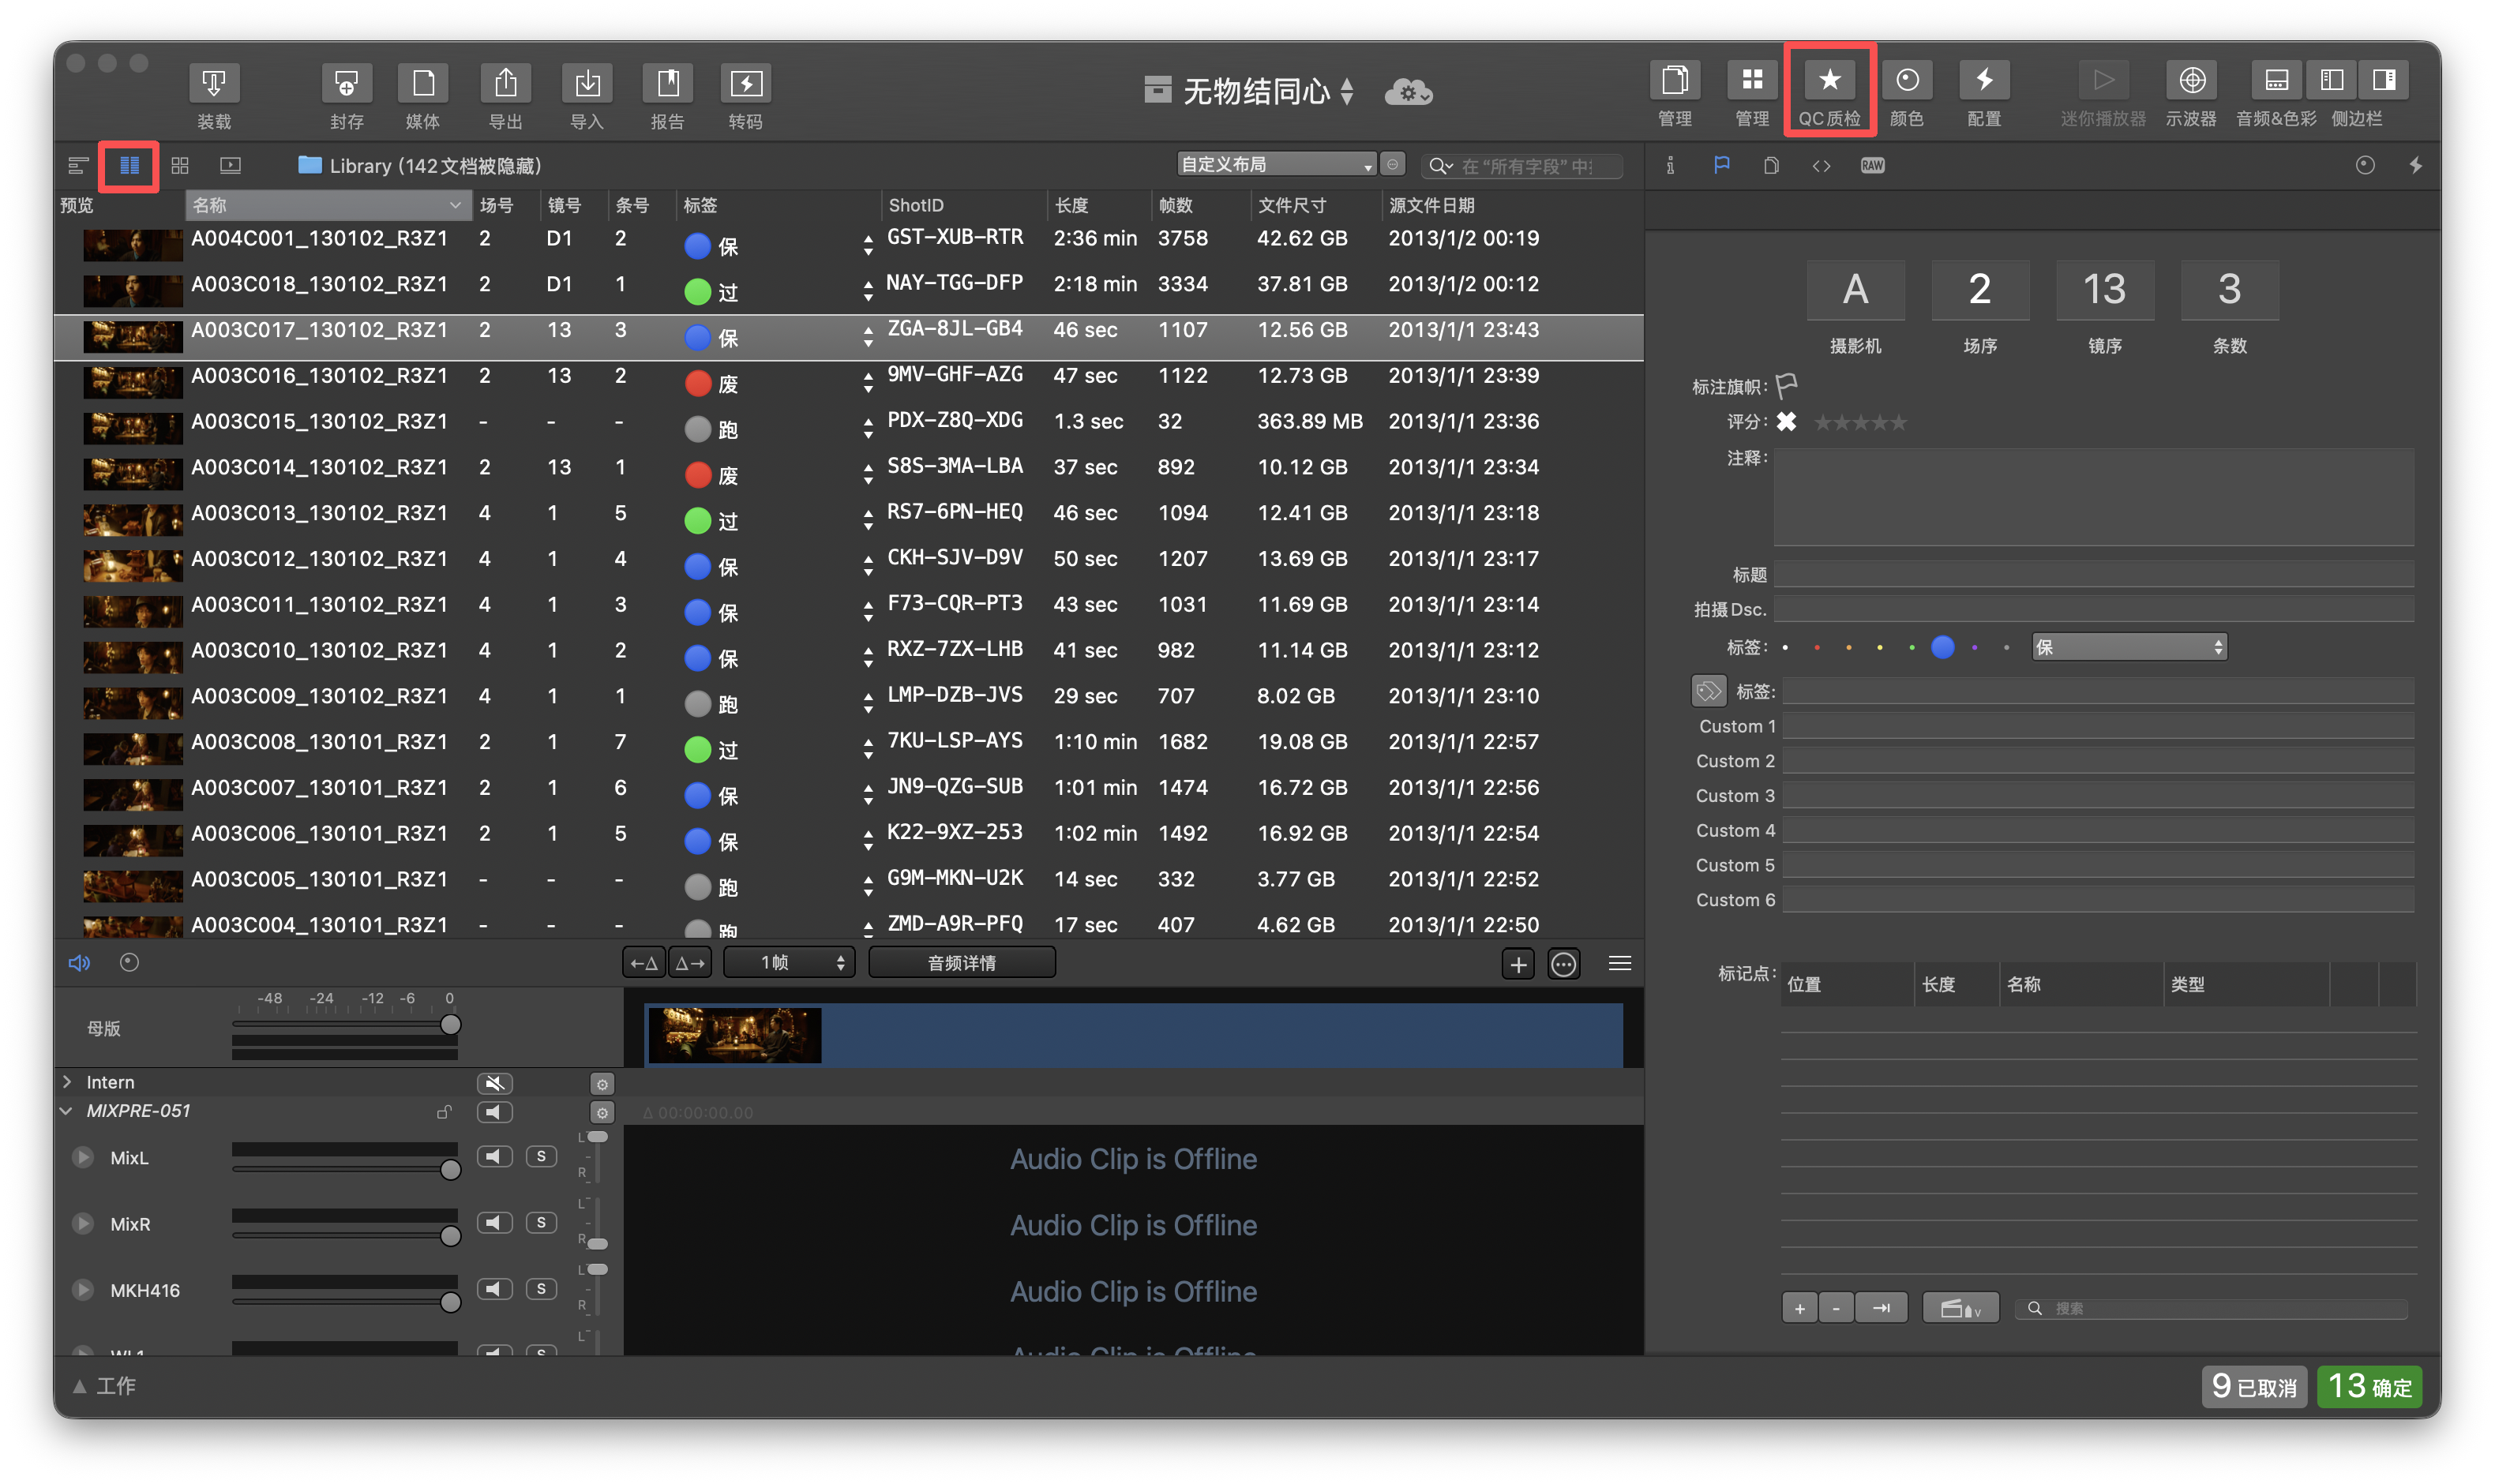
\includegraphics[width=0.95\linewidth]{可以点击qc质检，然后左上角选择列表视图快速打场镜次.png}
    \caption{在 QC 质检模式的列表视图下快速录入场记元数据}
\end{figure}

\subsection{同步音频}
如果现场是双系统独立录音，你需要将录音文件拷入备好的 Sound 文件夹。选中匹配的视频和音频，点击右下角的“配置”图标或在下方音频面板右键，选择“同步音频...”。只要现场时码器正常，软件便会自动将音频挂载到视频上。
\begin{figure}[H]
    \centering
    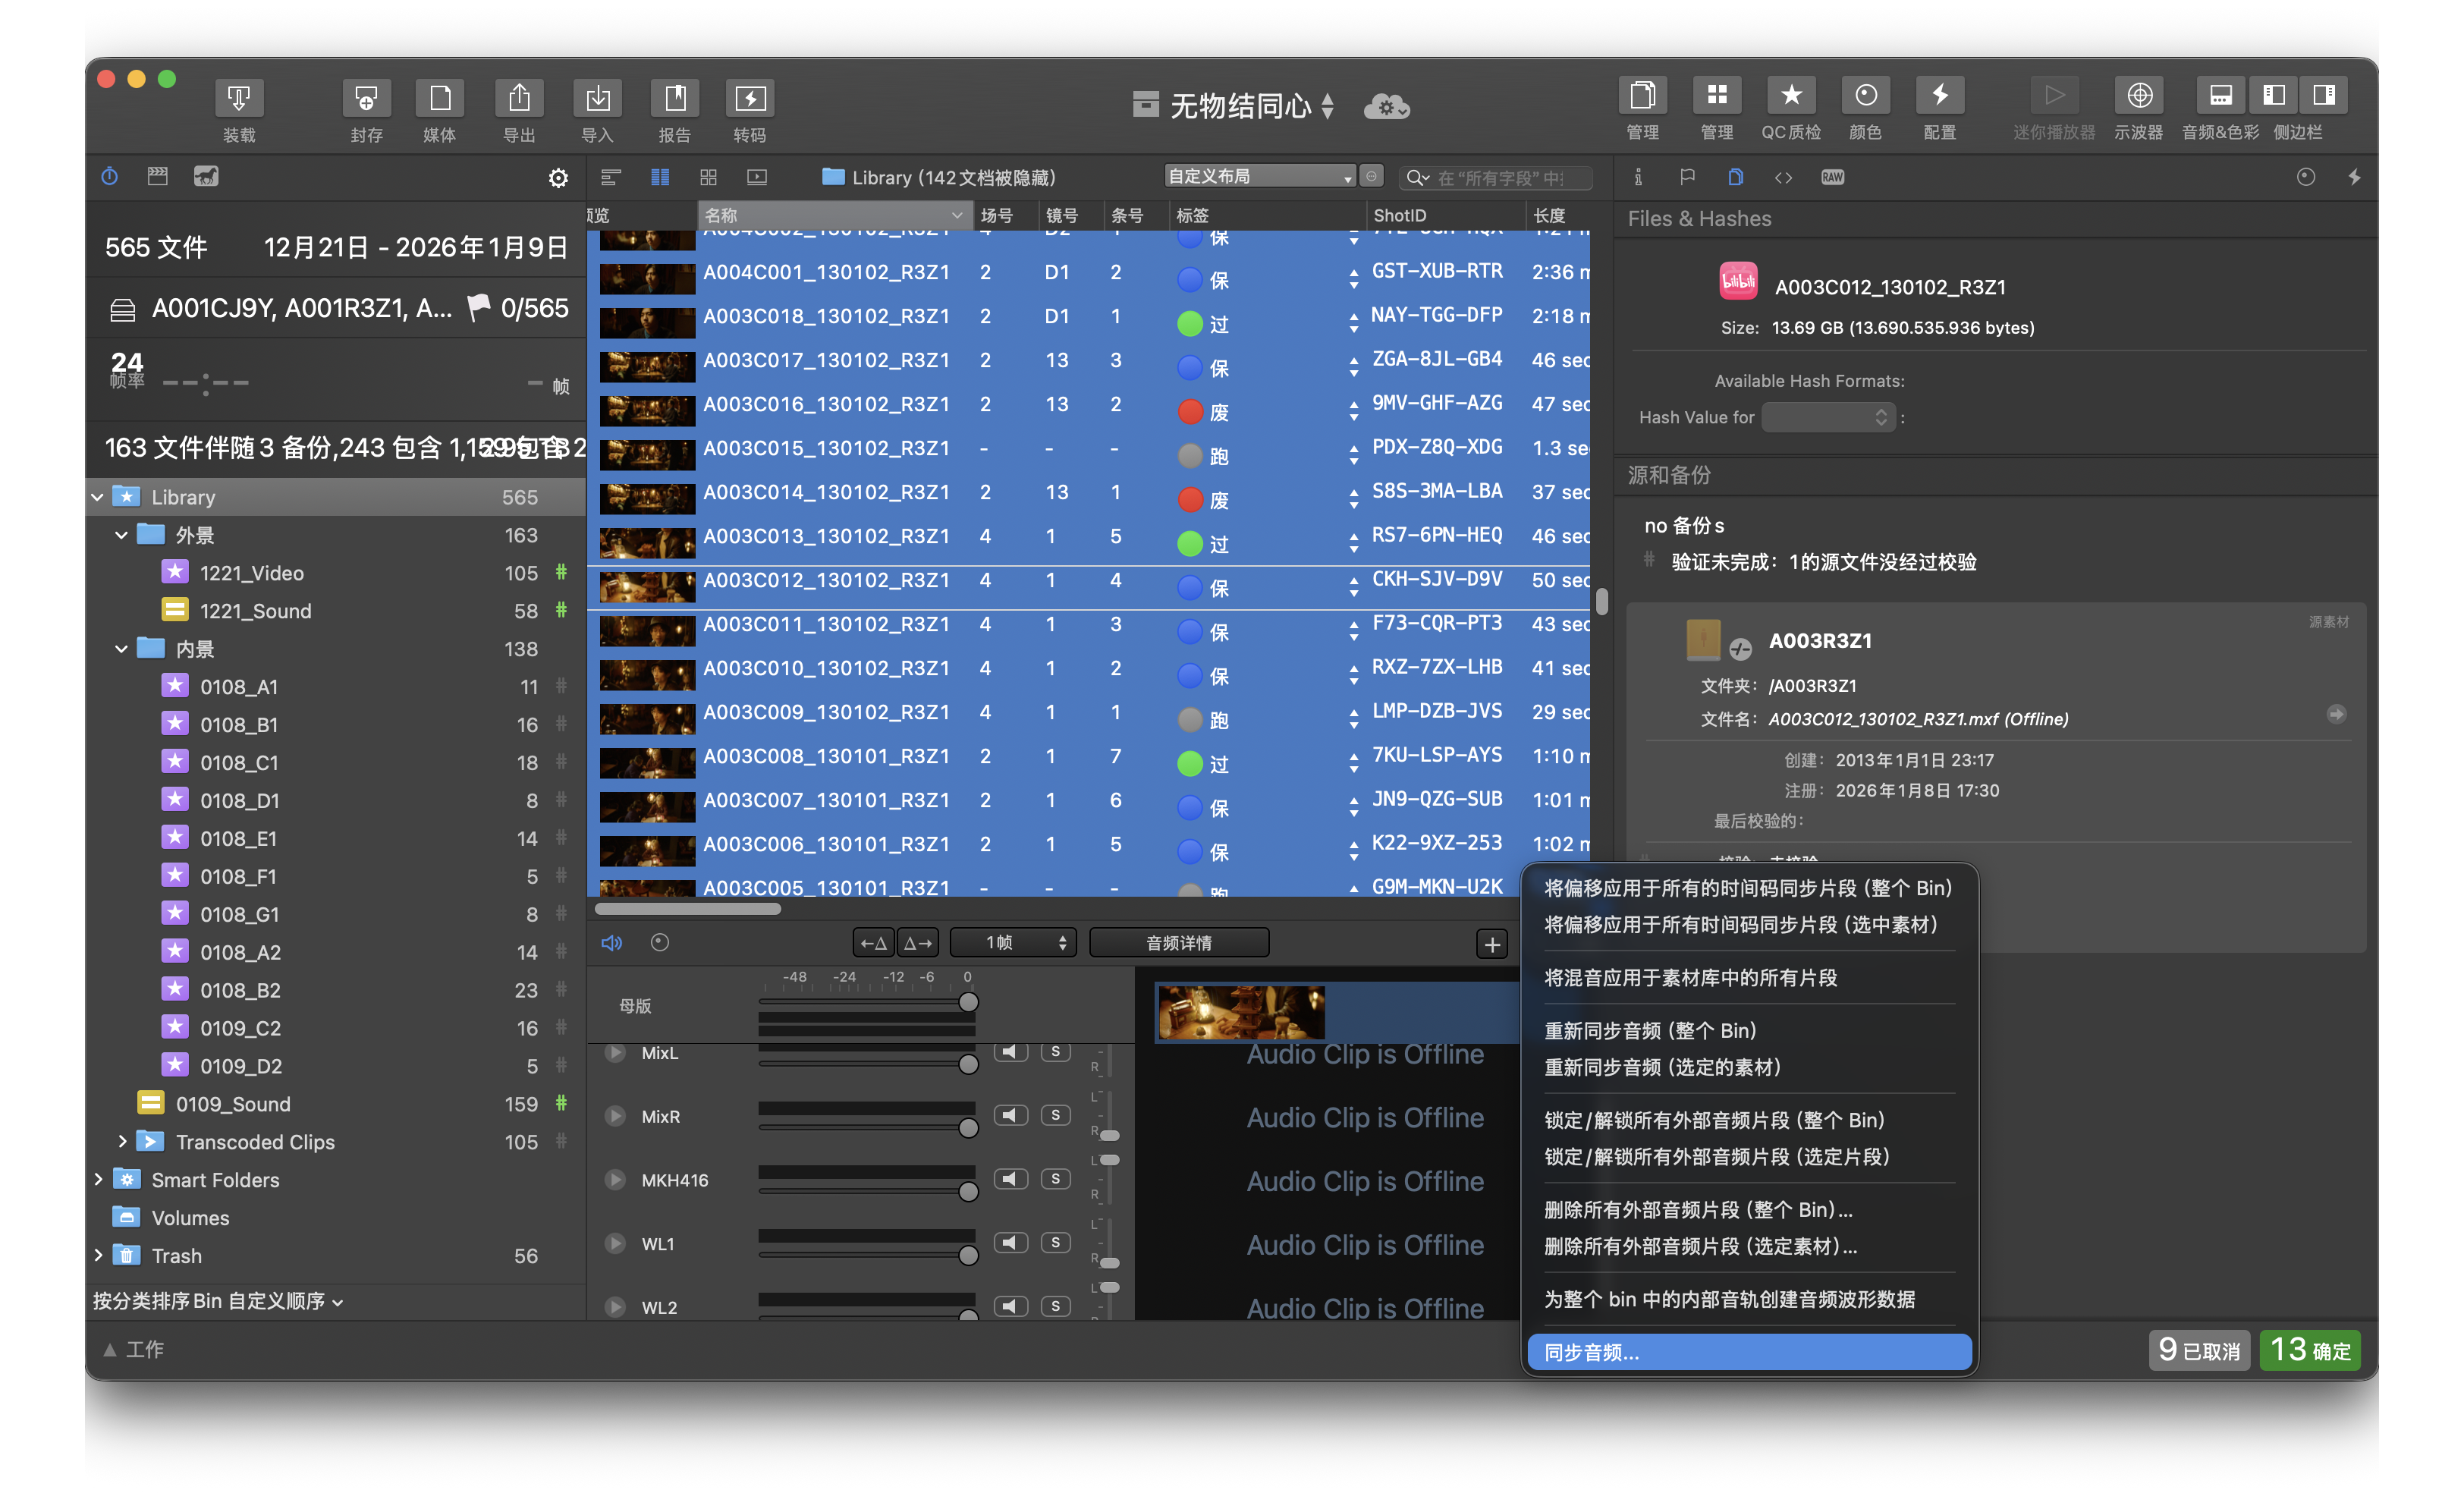
\includegraphics[width=0.95\linewidth]{点击右上角，同步音频的操作.png}
    \caption{在音频面板设置中选择“同步音频”}
\end{figure}

\subsection{交接卡}
确认备份无误后，把大力胶标签重新打好，交还给摄影助理去格式化。


\newpage
% ==========================================
% 第五章 现场信号与监看
% ==========================================
\section{现场信号与监看 (Live Signal \& Monitoring)}
\label{sec:live_monitoring}

除了数据管理，DIT 还负责现场视频信号的分发与监看质量的管理，确保导演和摄影指导看到准确的画面。

\subsection{DIT 现场视频管理逻辑架构}
下图展示了一个标准的学生剧组 DIT 现场视频信号流与数据流逻辑。
\begin{figure}[H]
    \centering
    \includegraphics[width=0.95\linewidth]{DIT现场视频管理方案.png}
    \caption{学生剧组 DIT 现场视频管理逻辑流程图}
\end{figure}

\subsection{信号流程解析}
\begin{itemize}
    \item \textbf{信号源头：} 摄影机输出 SDI 或 HDMI 信号。
    \item \textbf{核心枢纽：} 信号进入视频矩阵/分发器 (Video Router/DA)。
    \item \textbf{分发路径：}
    \begin{itemize}
        \item \textbf{DIT 端：} 一路信号给到 DIT 工作站，用于实时分析、套用 LUT 和色彩管理 (LiveGrade)。
        \item \textbf{导演/DP 端：} 一路给到经过校色的大监。
        \item \textbf{移动端：} 一路连接无线图传发射器，供导演手持监视器使用。
        \item \textbf{回放端：} 一路连接录机 (VTR) 用于现场回放。
    \end{itemize}
\end{itemize}

\subsection{预览与套 LUT}
在 Silverstack 顶部菜单找到“颜色”面板，你可以在预览阶段直接给原素材（灰片）套上对应的监看 LUT。这样不仅方便在现场进行高质量回放，后续输出代理时也会直接带上调色效果。


\newpage
% ==========================================
% 第六章 转码与交付
% ==========================================
\section{转码与交付 (Transcoding \& Deliverables)}
\label{sec:transcoding}

DIT 工作流的最后一步是生成供剪辑、审阅使用的代理文件和包含所有元数据的报告。

\subsection{Silverstack 转码代理}
在没有现场剪辑、对后期不着急的情况下，建议等一批素材结束或收工后再统一导出代理，因为导出时会大量占用系统资源。当然有空就导出是对的，可以快速查看素材质量并方便回放。

点击顶部工具栏的“转码”按钮，首先建议新建一个转码预设。对于烧录信息（Burn-Ins），把重要的信息写上就好，可以按照个人的习惯配置来定，比如说下面一种：
\begin{itemize}
    \item \textbf{左上}：场 / 镜 / 次信息
    \item \textbf{正上}：记录“过/保/废”状态
    \item \textbf{右上}：项目名
    \item \textbf{左下}：源时间码
    \item \textbf{正下}：注释补充
    \item \textbf{右下}：源文件名
\end{itemize}

\begin{figure}[H]
    \centering
    \begin{minipage}[t]{0.48\linewidth}
        \centering
        \includegraphics[width=\linewidth]{首先建议新建转码预设.png}
        \caption{新建并自定义包含场记板信息的转码预设}
    \end{minipage}%
    \hfill%
    \begin{minipage}[t]{0.48\linewidth}
        \centering
        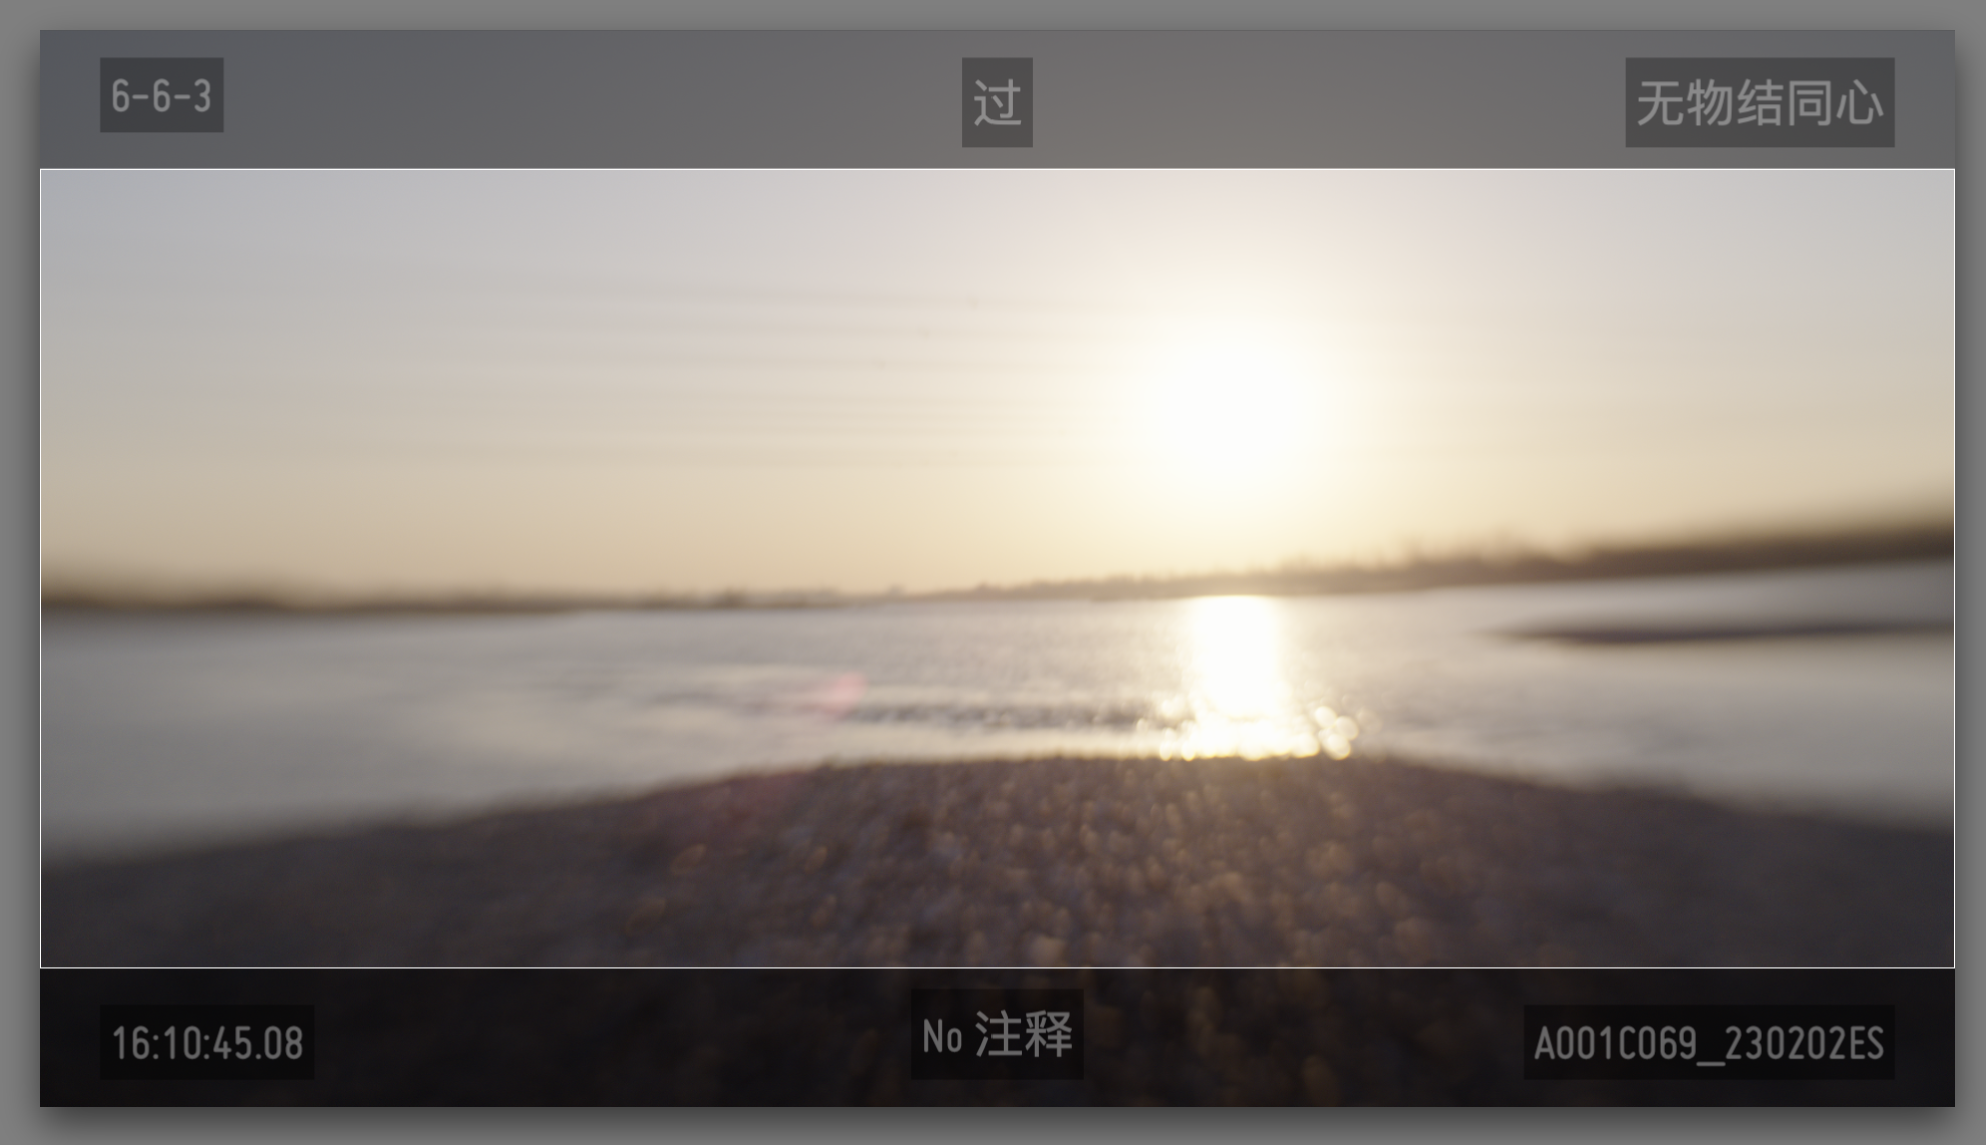
\includegraphics[width=\linewidth]{转码预设最终结果带遮幅.png} 
        \caption{自定义烧入数据的最终结果预览（含遮幅）}
    \end{minipage}
\end{figure}

预设建好后，选择将单个素材导出到盘中每一天对应的 Proxy 文件夹下。
\begin{figure}[H]
    \centering
    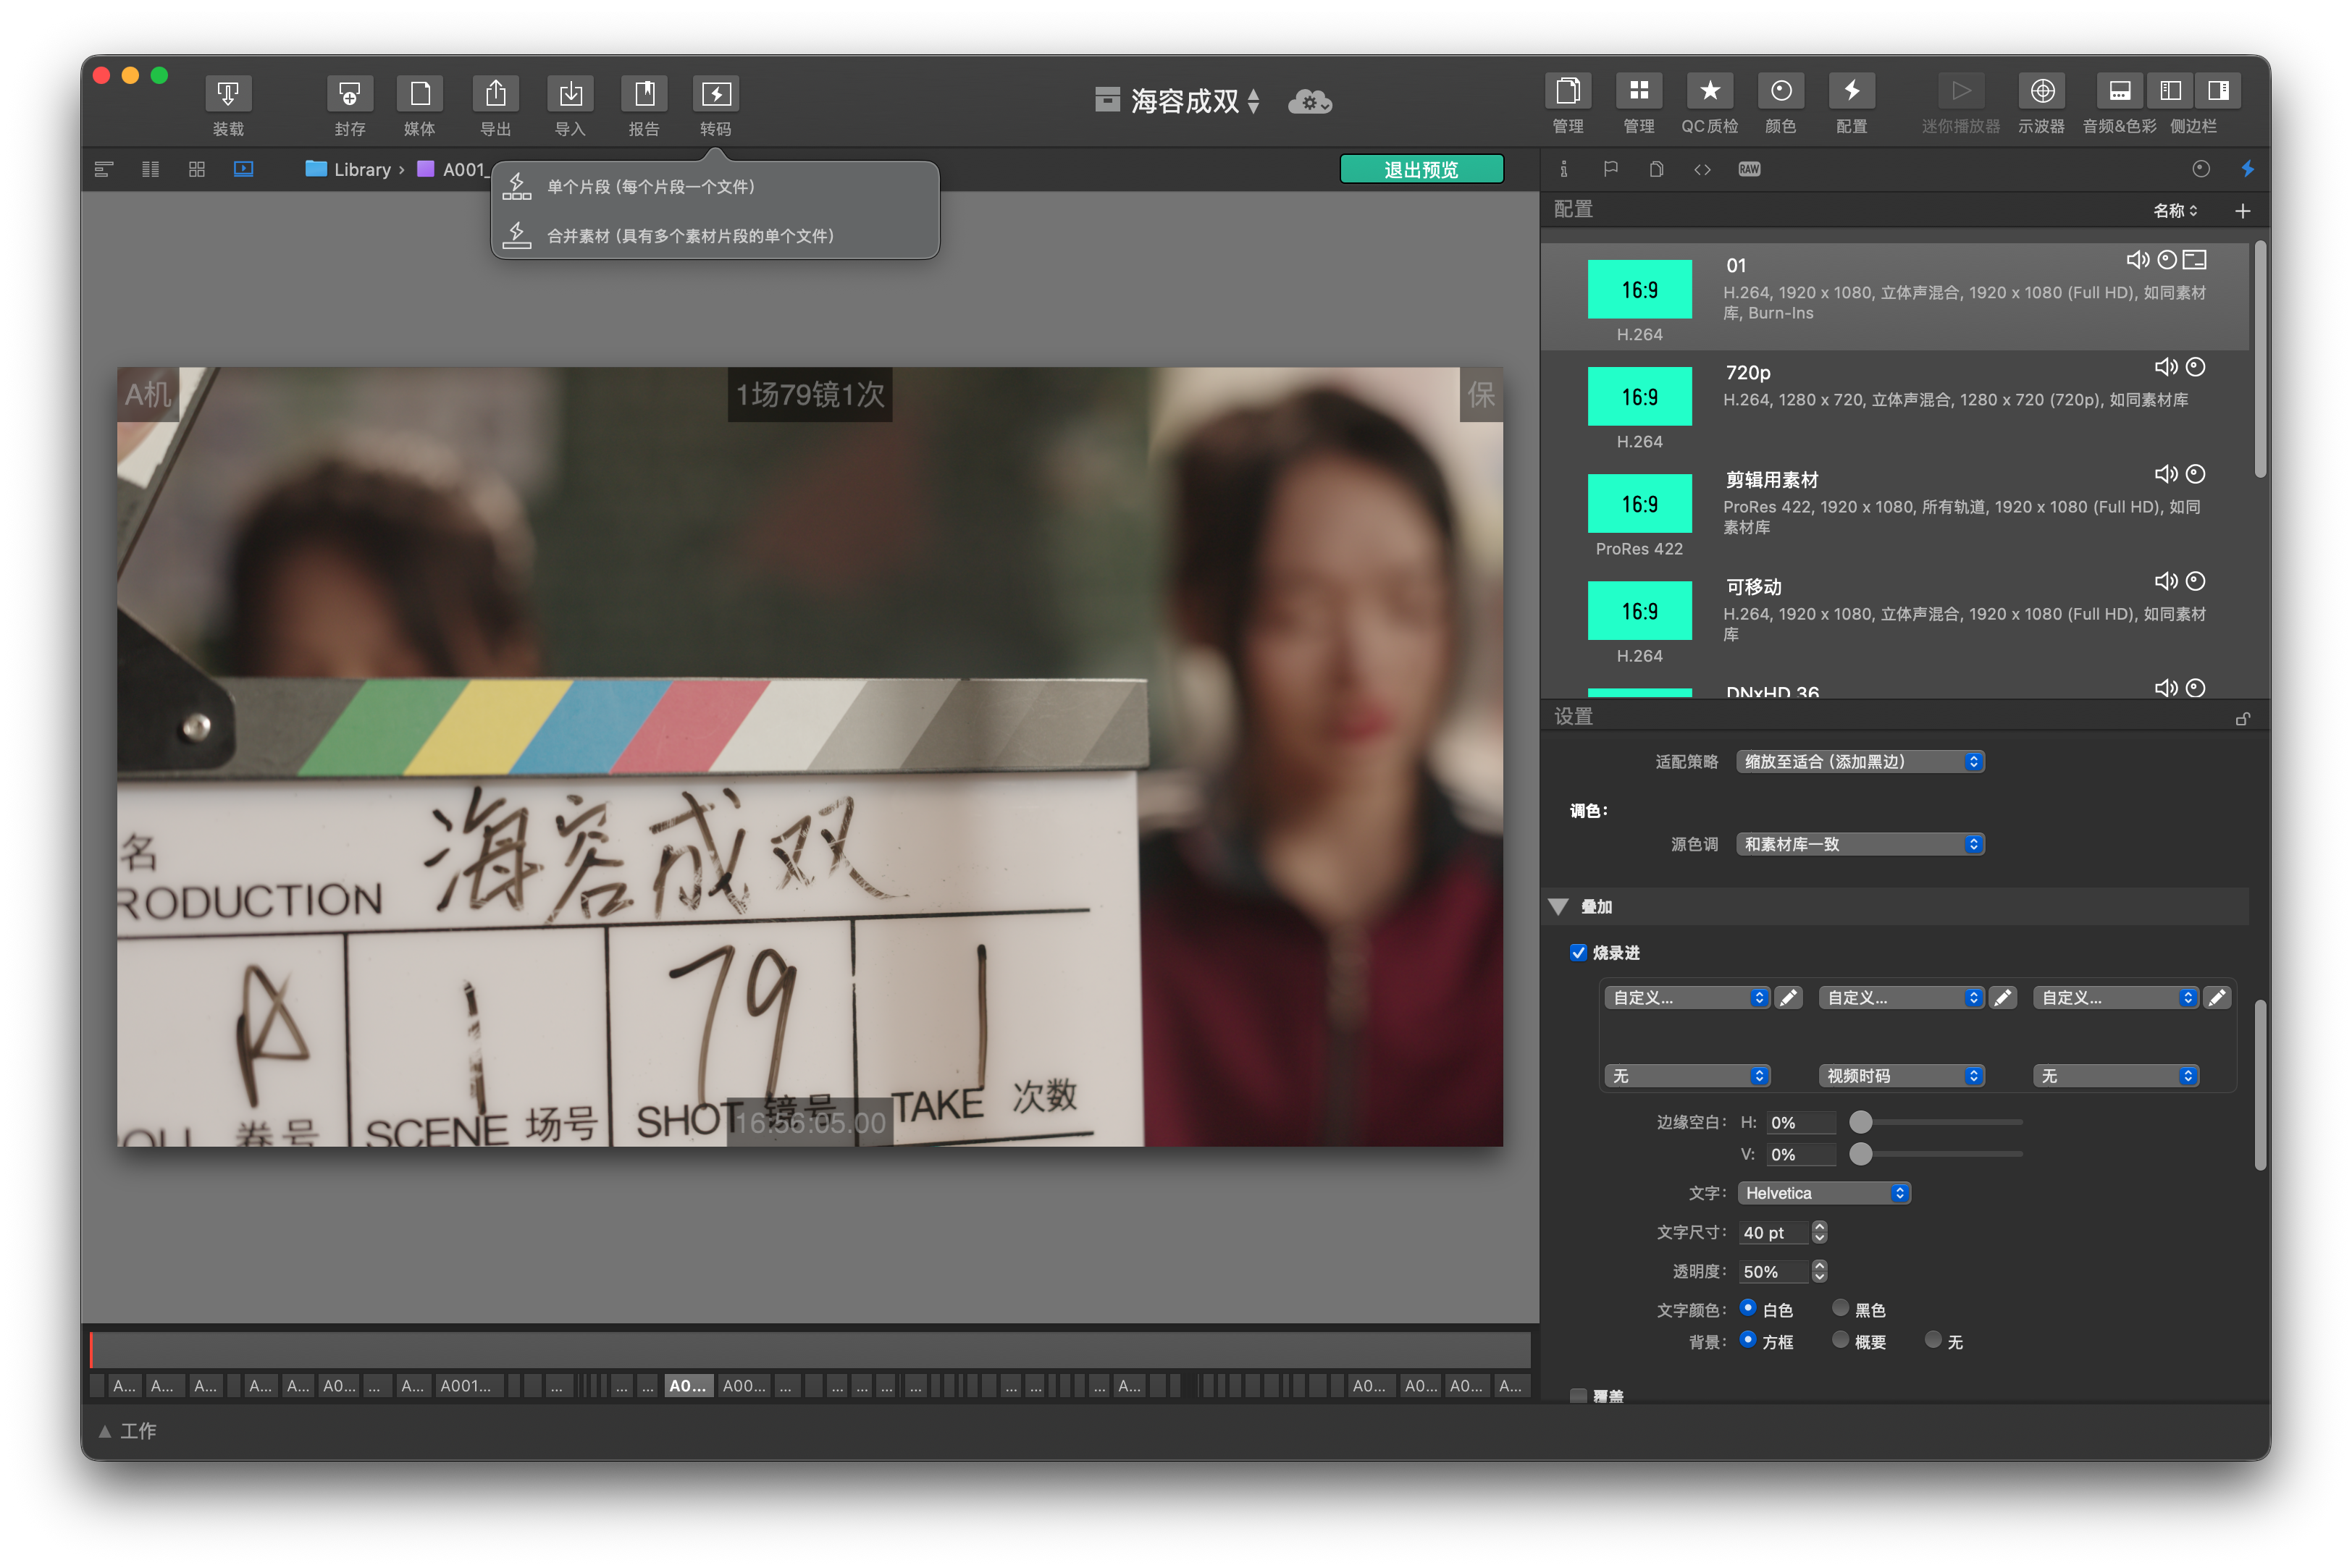
\includegraphics[width=0.9\linewidth]{选择转码导出单个素材.png}
    \caption{选择单个片段（每个片段一个文件）进行代理导出}
\end{figure}

\subsection{生成报告与 XML 交付}
确认所有实物卡整理好交给跟机员后，在 Library 选中拷完的 Bin。在最上面一排的工具栏中，你可以找到导出报告和 XML 的入口。
\begin{figure}[H]
    \centering
    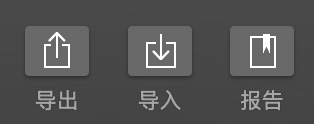
\includegraphics[width=0.4\linewidth]{导出导入报告.png}
    \caption{工具栏中的导出与报告按钮}
\end{figure}

生成的 PDF 报告包含缩略图、时码和格式。每天收工发到剧组群里，如果导演没有特别反对组员看到报告的话，我会这么干，毕竟这是你专业度的体现，也是“我确实干活了”的铁证。同时，根据后期使用的软件导出对应的 XML（达芬奇/FCP/PR），放在盘的 Metadata 文件夹里。
\begin{figure}[H]
    \centering
    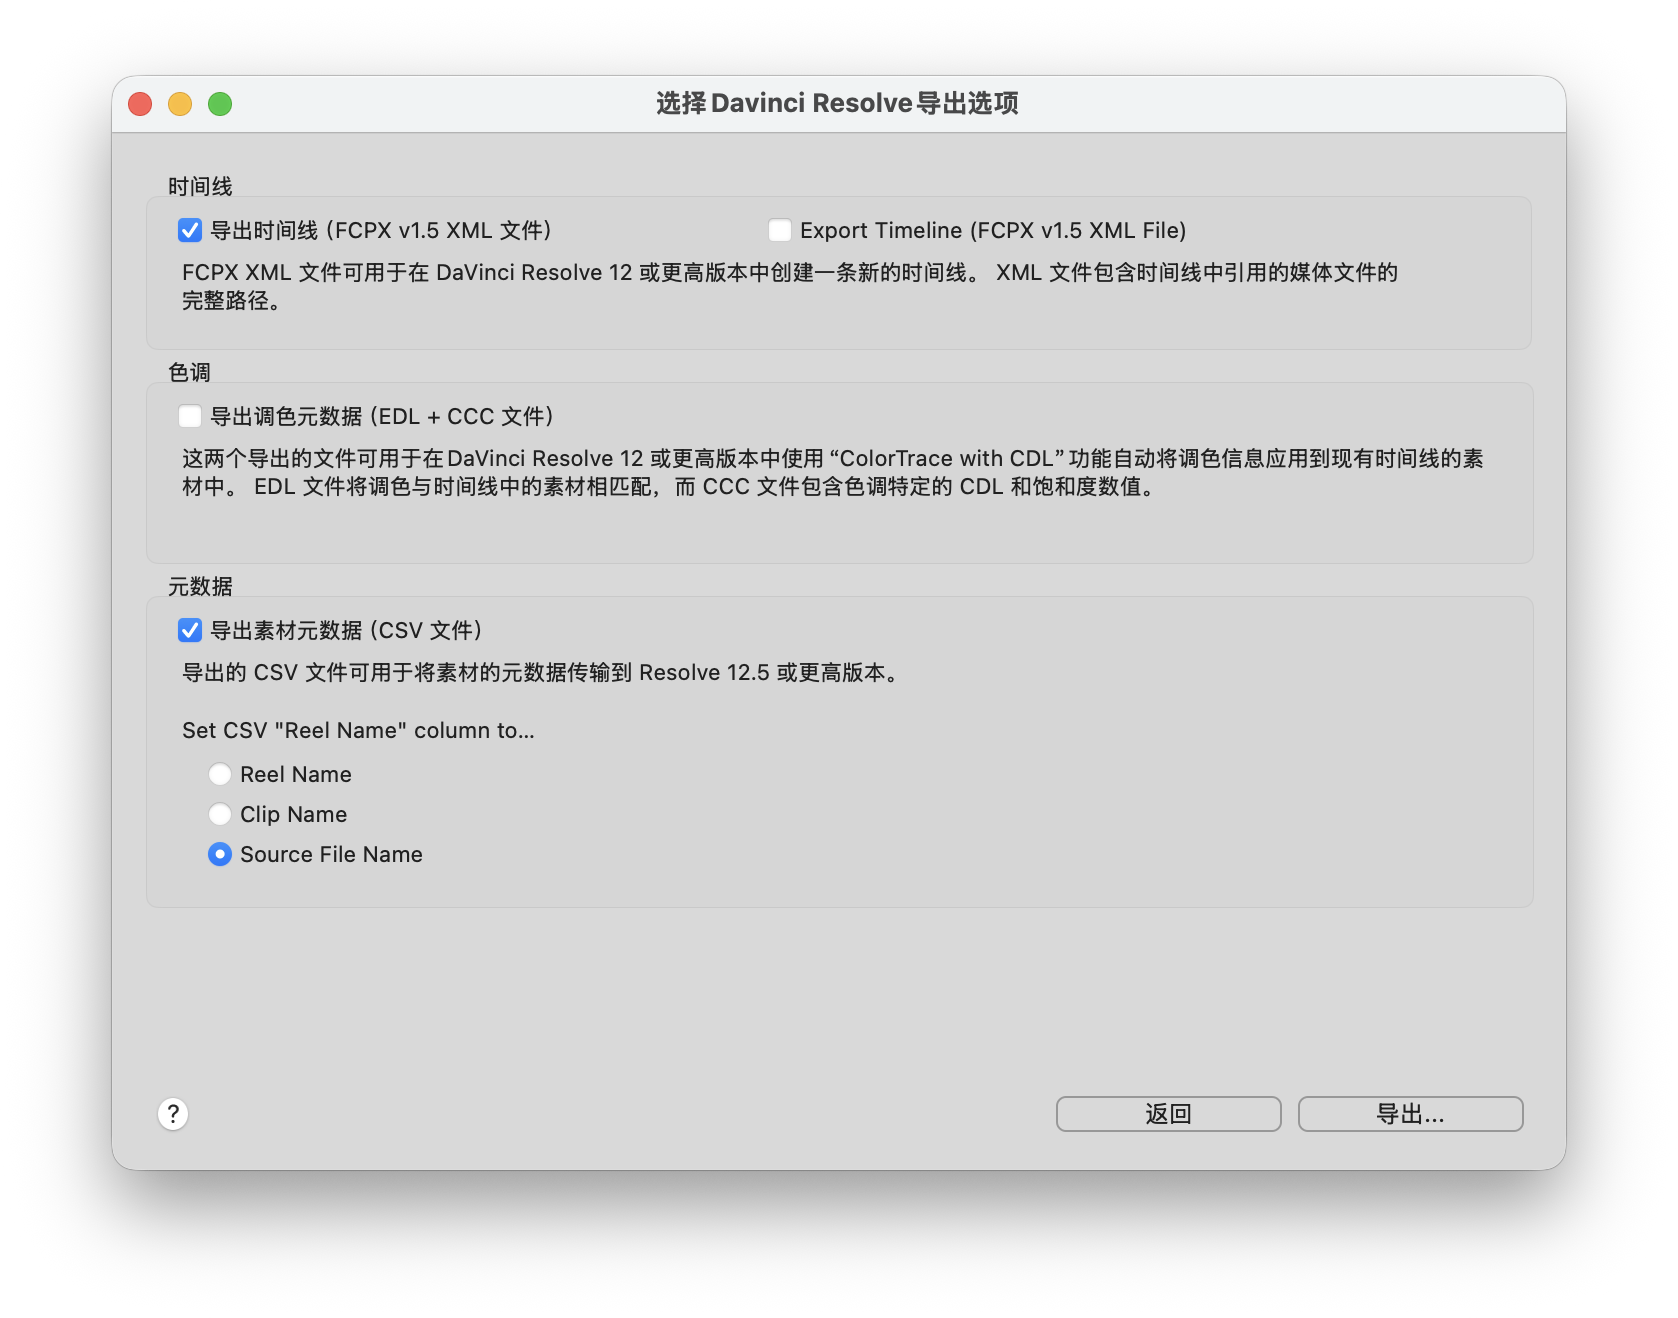
\includegraphics[width=0.8\linewidth]{XML 导出设置参考.png}
    \caption{后期软件 XML 导出设置参考}
\end{figure}


\newpage
% ==========================================
% 第七章 疑难解答与进阶话题
% ==========================================
\section{疑难解答与进阶话题 (Troubleshooting \& Advanced Topics)}
\label{sec:advanced}

\subsection{达芬奇 (DaVinci Resolve) 元数据导入与代理交付}
\label{subsec:davinci_proxy} 

在某些特殊情况下（例如现场盘速太慢，导致 Silverstack 无法正常全速转码生成 Proxy 时），我强烈建议使用达芬奇来导出带有 Silverstack 元数据的代理文件。这不仅是 DIT 的备用方案，对于后续接手素材的剪辑师来说，前期的准备工作也是一样的。

首先，我们需要将 Silverstack 中整理好的场记信息（场、镜、次等）导入到达芬奇中。

\textbf{步骤 1：导入元数据} \\
在达芬奇的媒体池中选中你的素材，依次点击顶部菜单栏的：\texttt{文件 -> 导入元数据到 -> 媒体池}。
\begin{figure}[H]
    \centering
    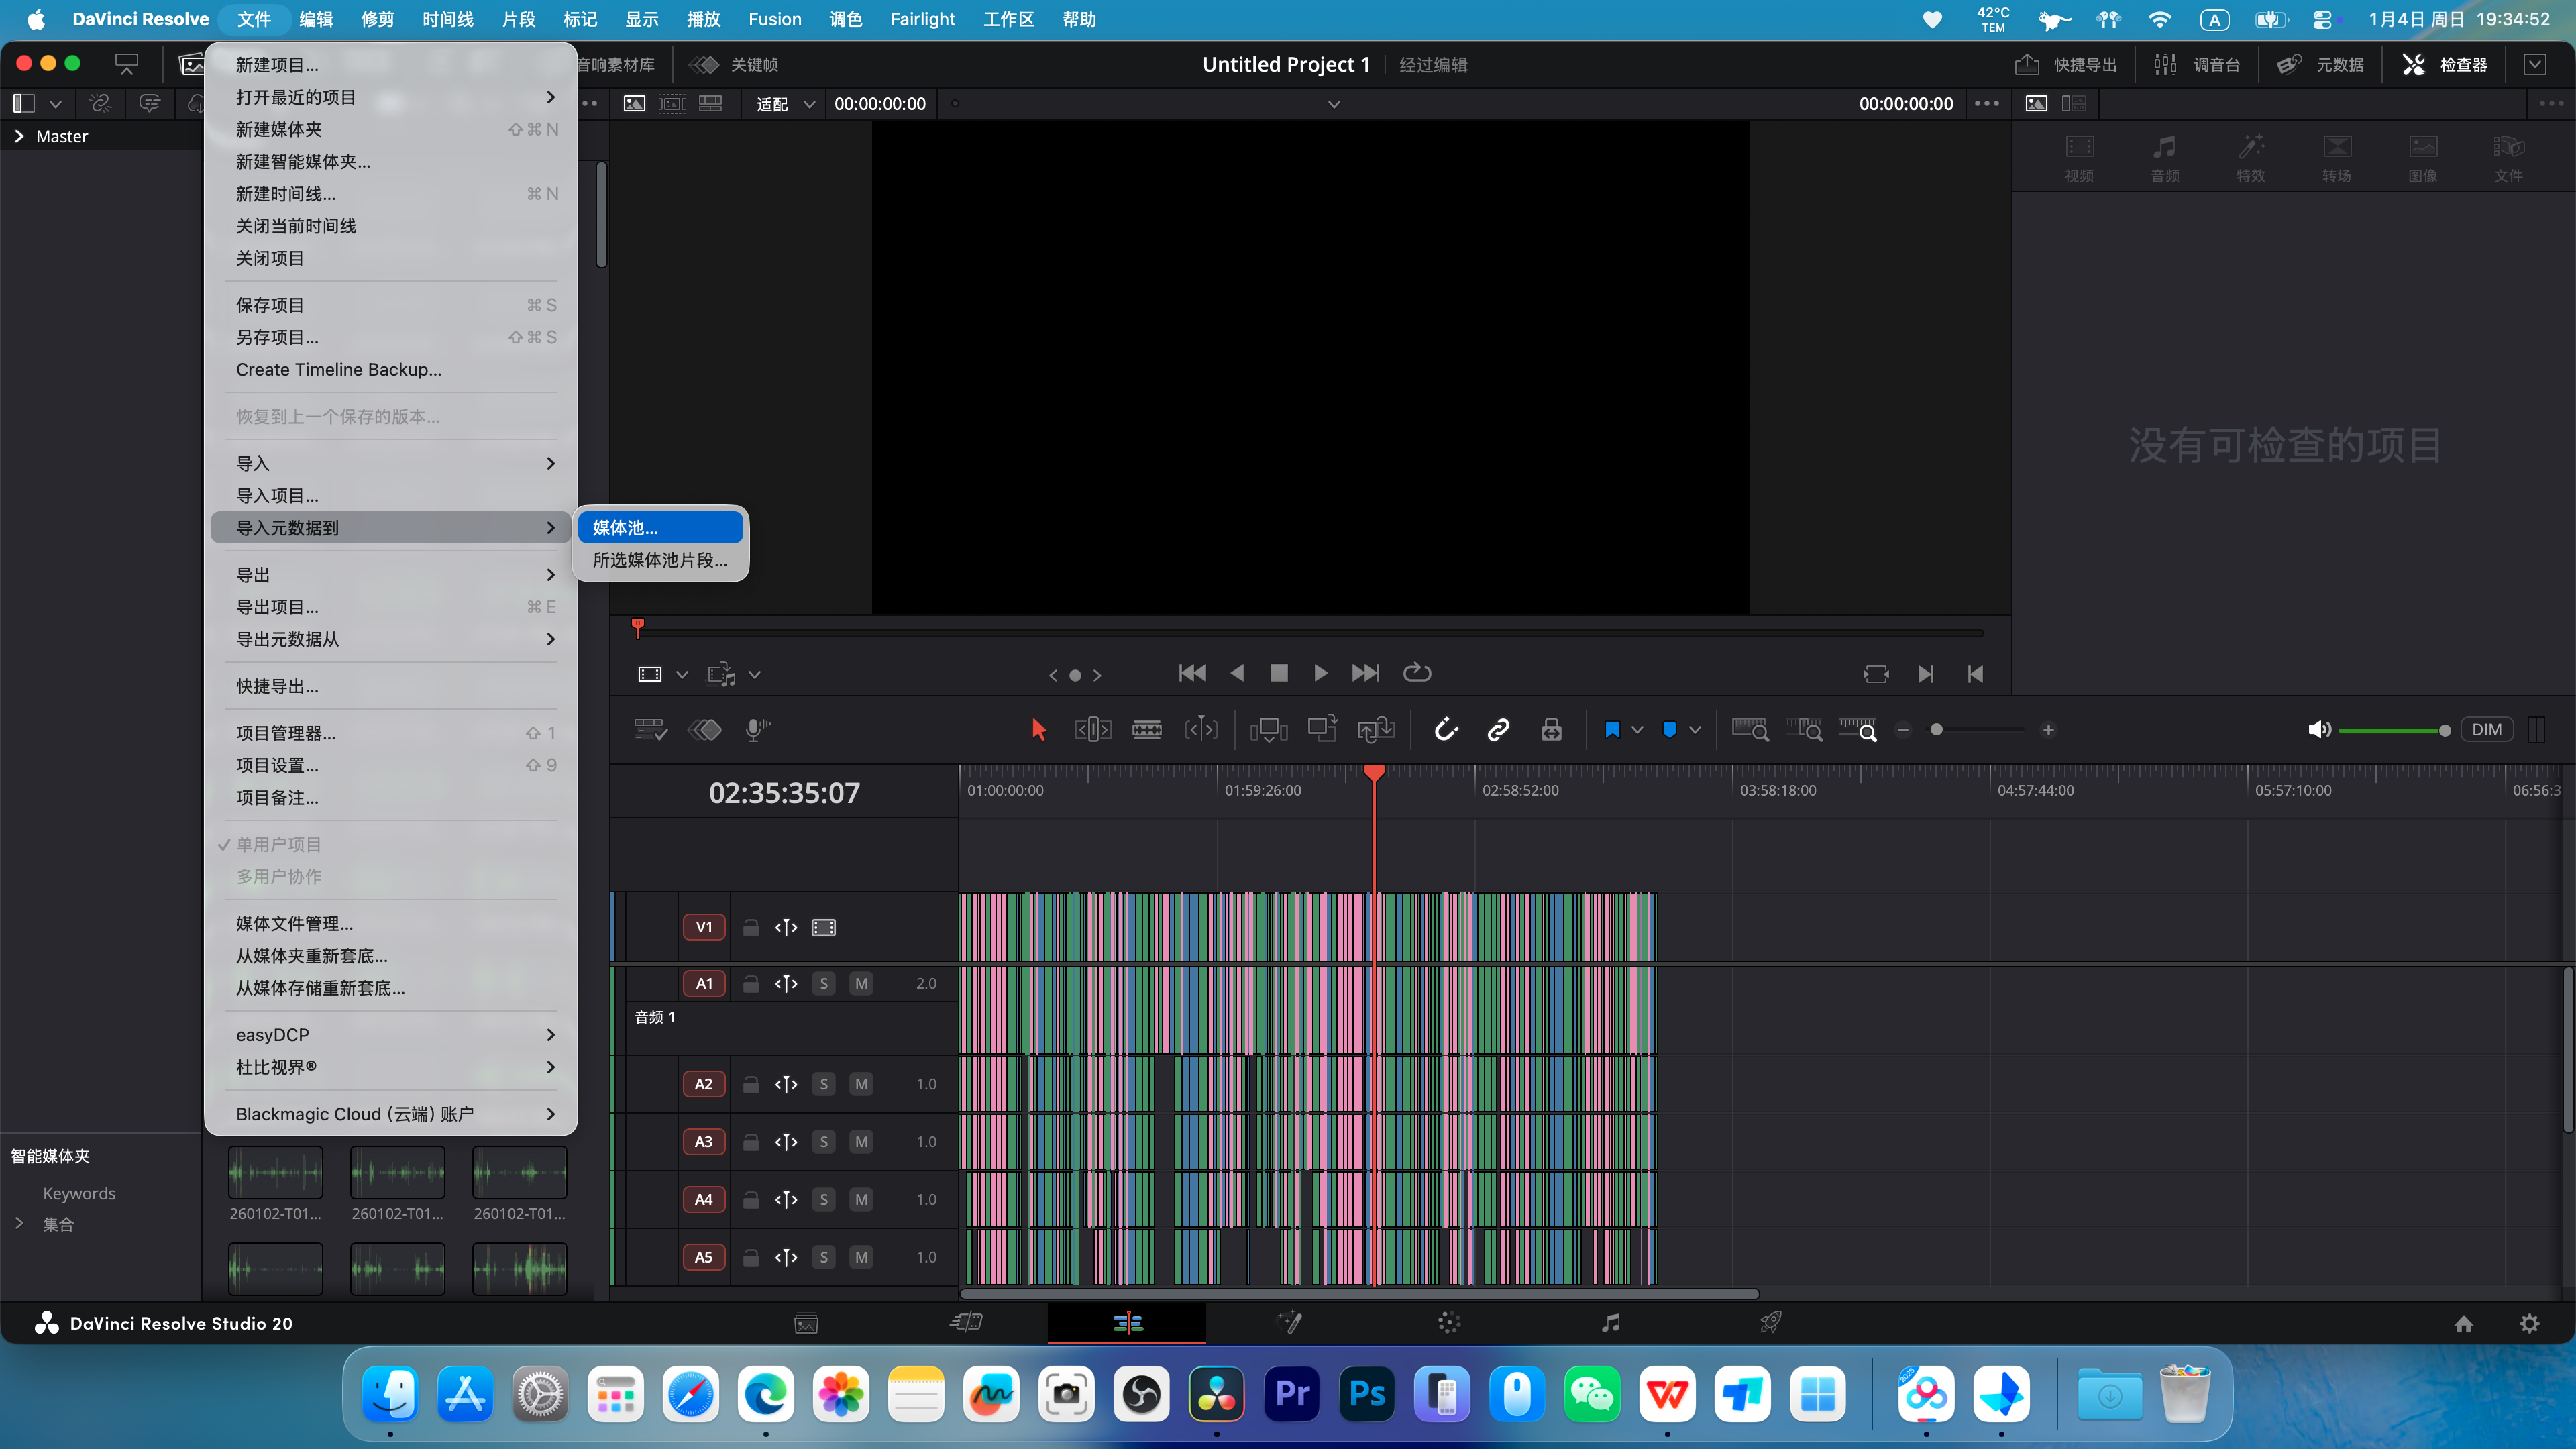
\includegraphics[width=0.9\linewidth]{打开达芬奇选择文件.png} 
    \caption{在达芬奇中选择导入元数据到媒体池}
\end{figure}

\textbf{步骤 2：选择 CSV 文件} \\
在弹出的窗口中，找到你之前用 Silverstack 导出的 Metadata 文件夹，选择里面的 \texttt{.csv} 文件（默认的命名为 \texttt{Library.csv}），点击打开。
\begin{figure}[H]
    \centering
    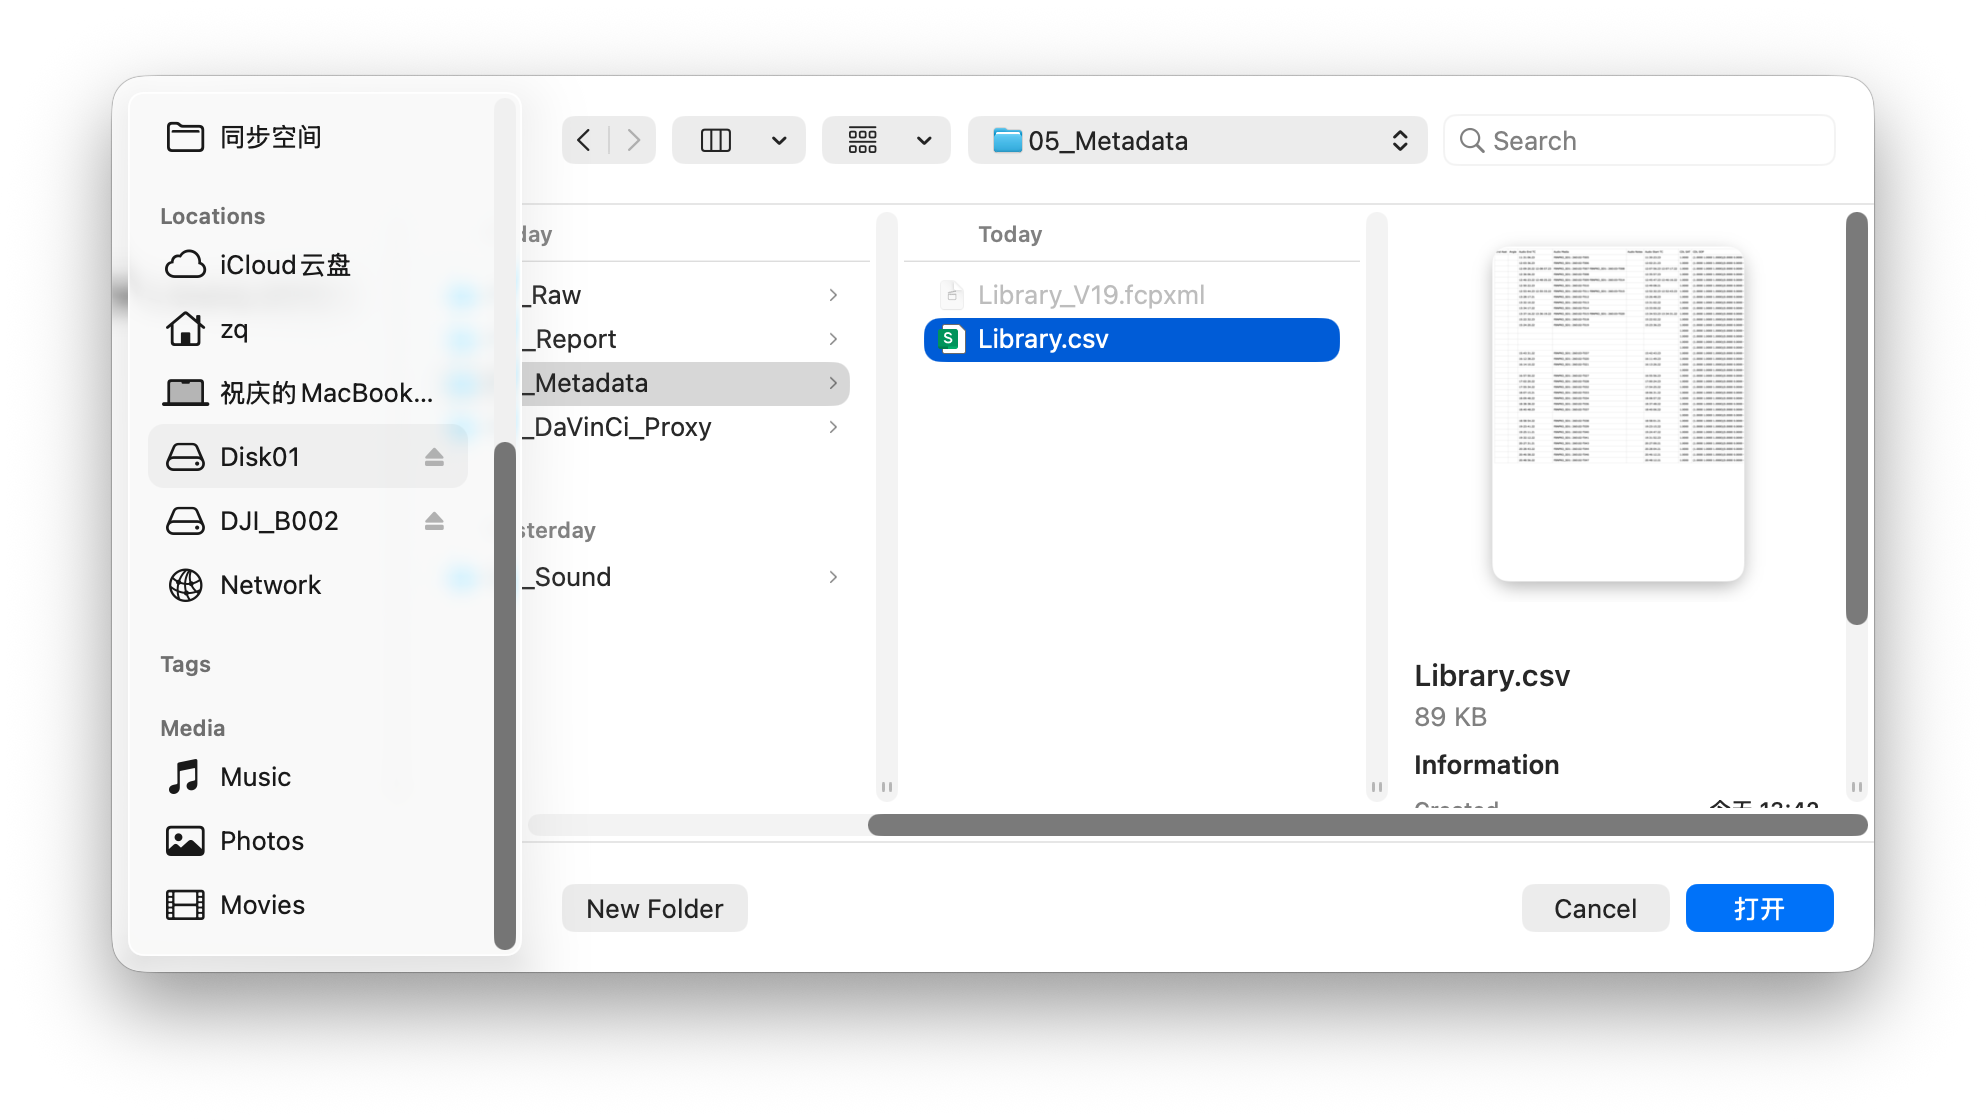
\includegraphics[width=0.85\linewidth]{选择metadata导出后的文件.png} 
    \caption{选择 Silverstack 生成的 Library.csv 文件}
\end{figure}

\textbf{步骤 3：匹配与合并选项} \\
在这个至关重要的界面，请确保勾选了正确的匹配规则，以便达芬奇能准确地将文本信息贴合到视频文件上。设置无误后，点击 OK。此时，你可以看到时间线上的片段变成了彩色，这正是前面我们在 Silverstack 中预设的“过、保、废”标签成功联动的体现。
\begin{figure}[H]
    \centering
    \begin{minipage}[t]{0.48\linewidth}
        \centering
        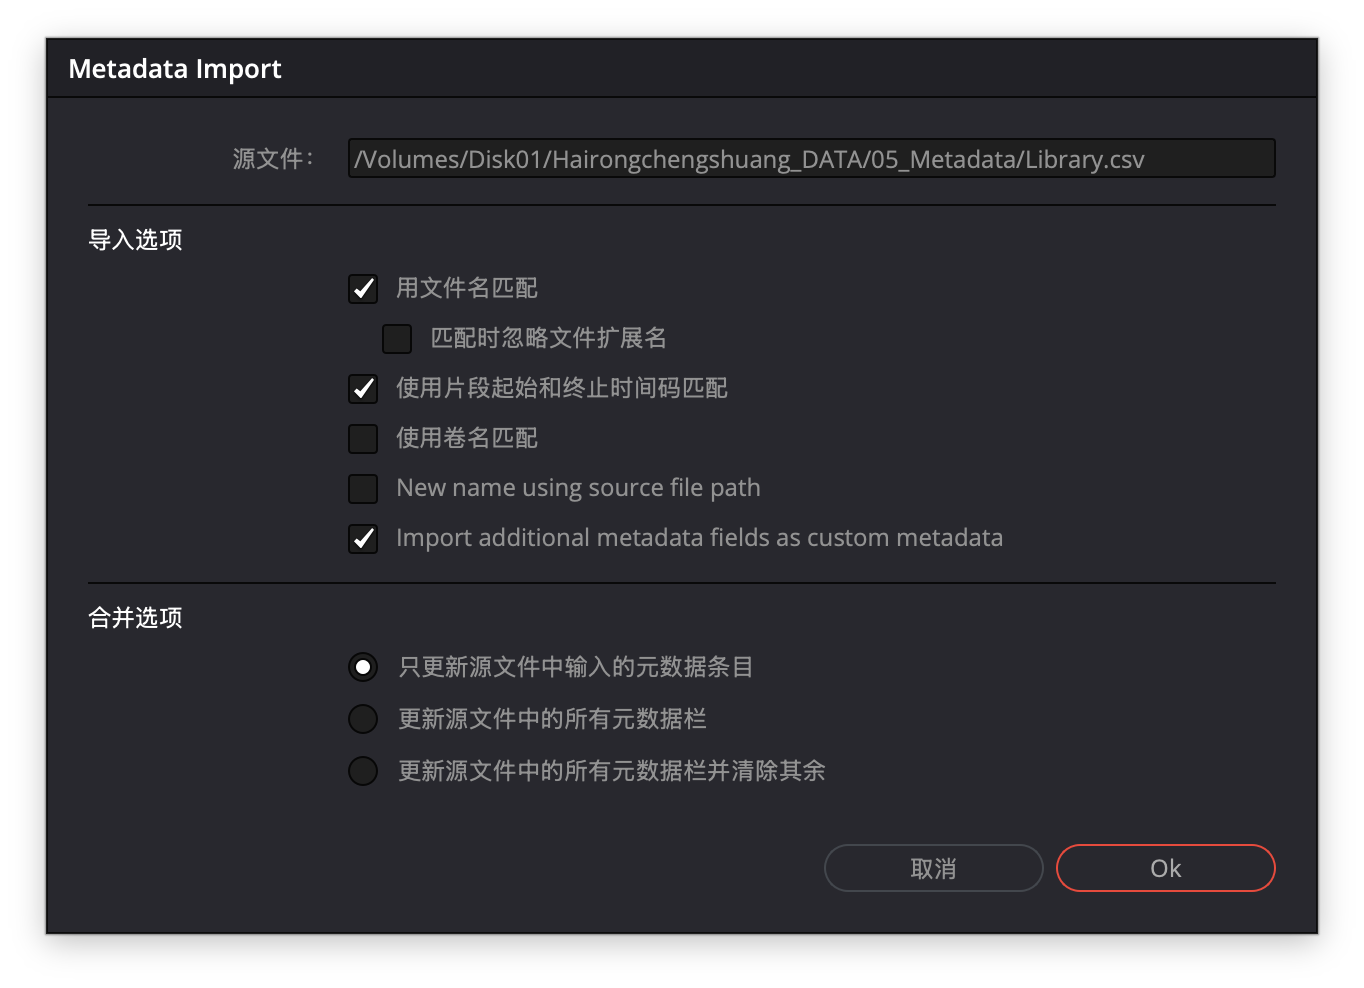
\includegraphics[width=\linewidth]{点击ok.png} 
        \caption{确认匹配选项并点击 OK}
    \end{minipage}%
    \hfill%
    \begin{minipage}[t]{0.48\linewidth}
        \centering
        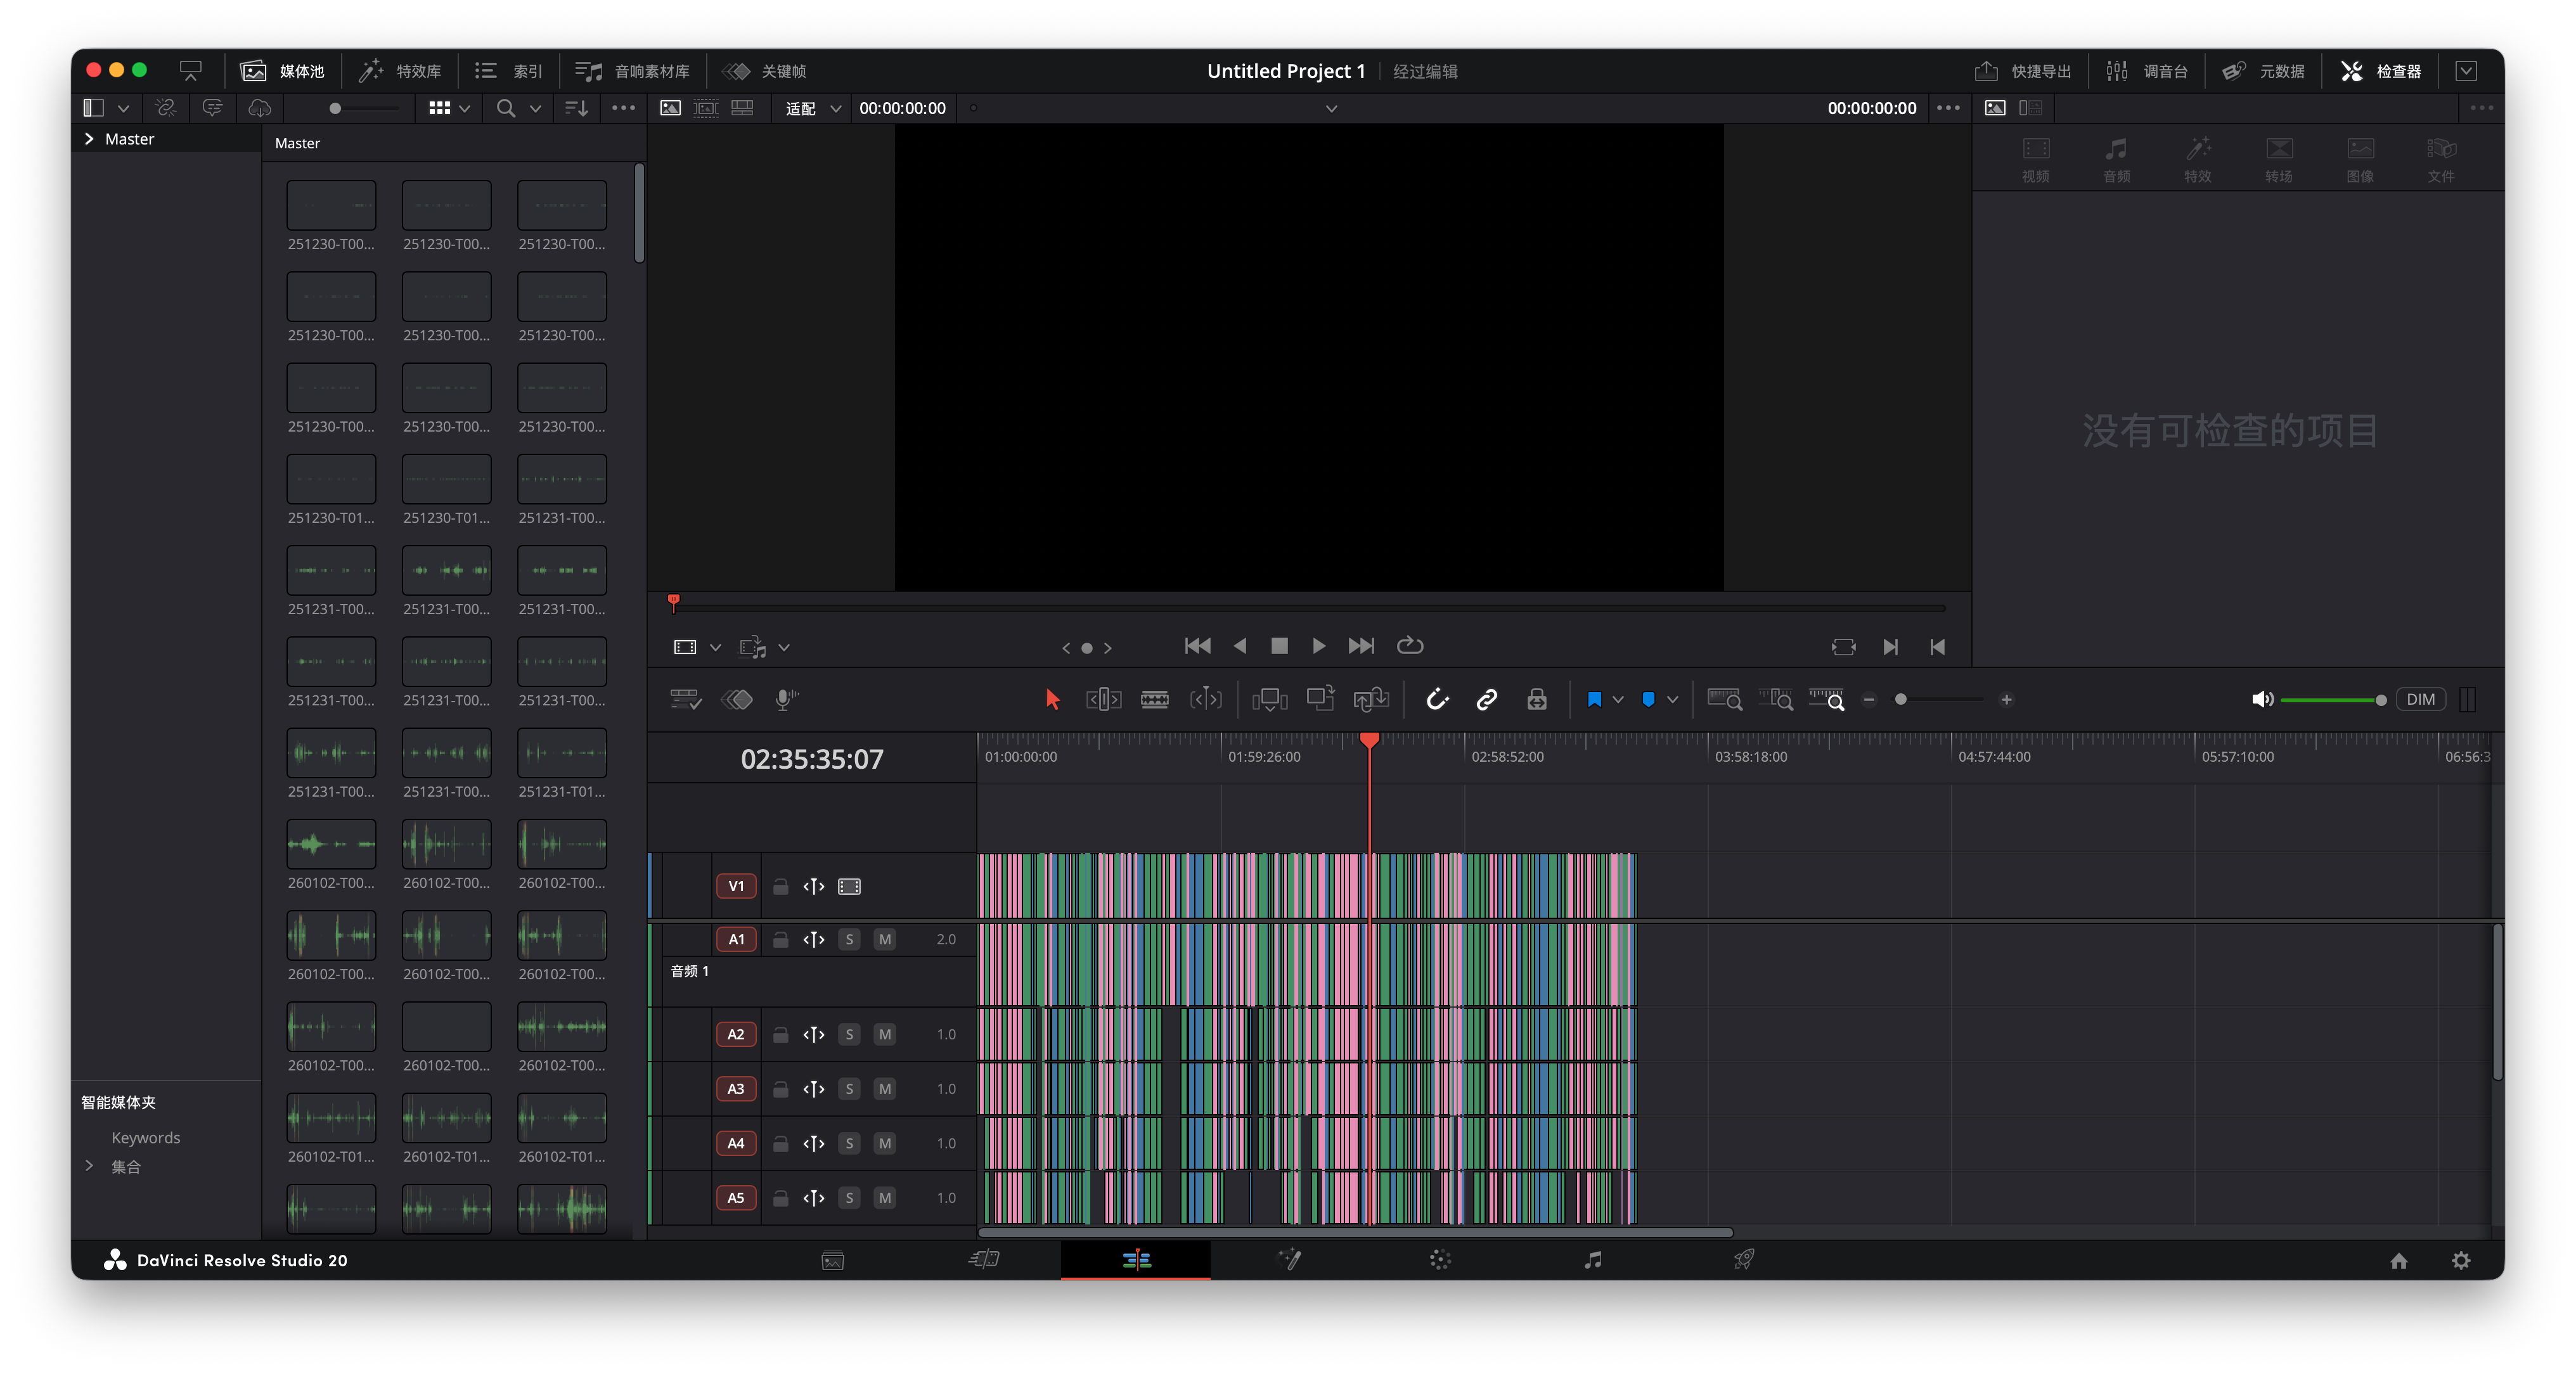
\includegraphics[width=\linewidth]{然后可以看到时间线上出现了彩色的片段，这个就是过报废的体现.png} 
        \caption{时间线上出现彩色片段，因为过报废采用了 Clip Color 的形式}
    \end{minipage}
\end{figure}

\textbf{步骤 4：设置数据烧录} \\
点击顶部菜单栏的 \texttt{工作区 -> 数据烧录}。在弹出的面板中，勾选你需要显示在画面上的信息。你可以调整右侧的字体大小和背景不透明度，确保字迹清晰且不遮挡关键画面。
\begin{figure}[H]
    \centering
    \begin{minipage}[t]{0.48\linewidth}
        \centering
        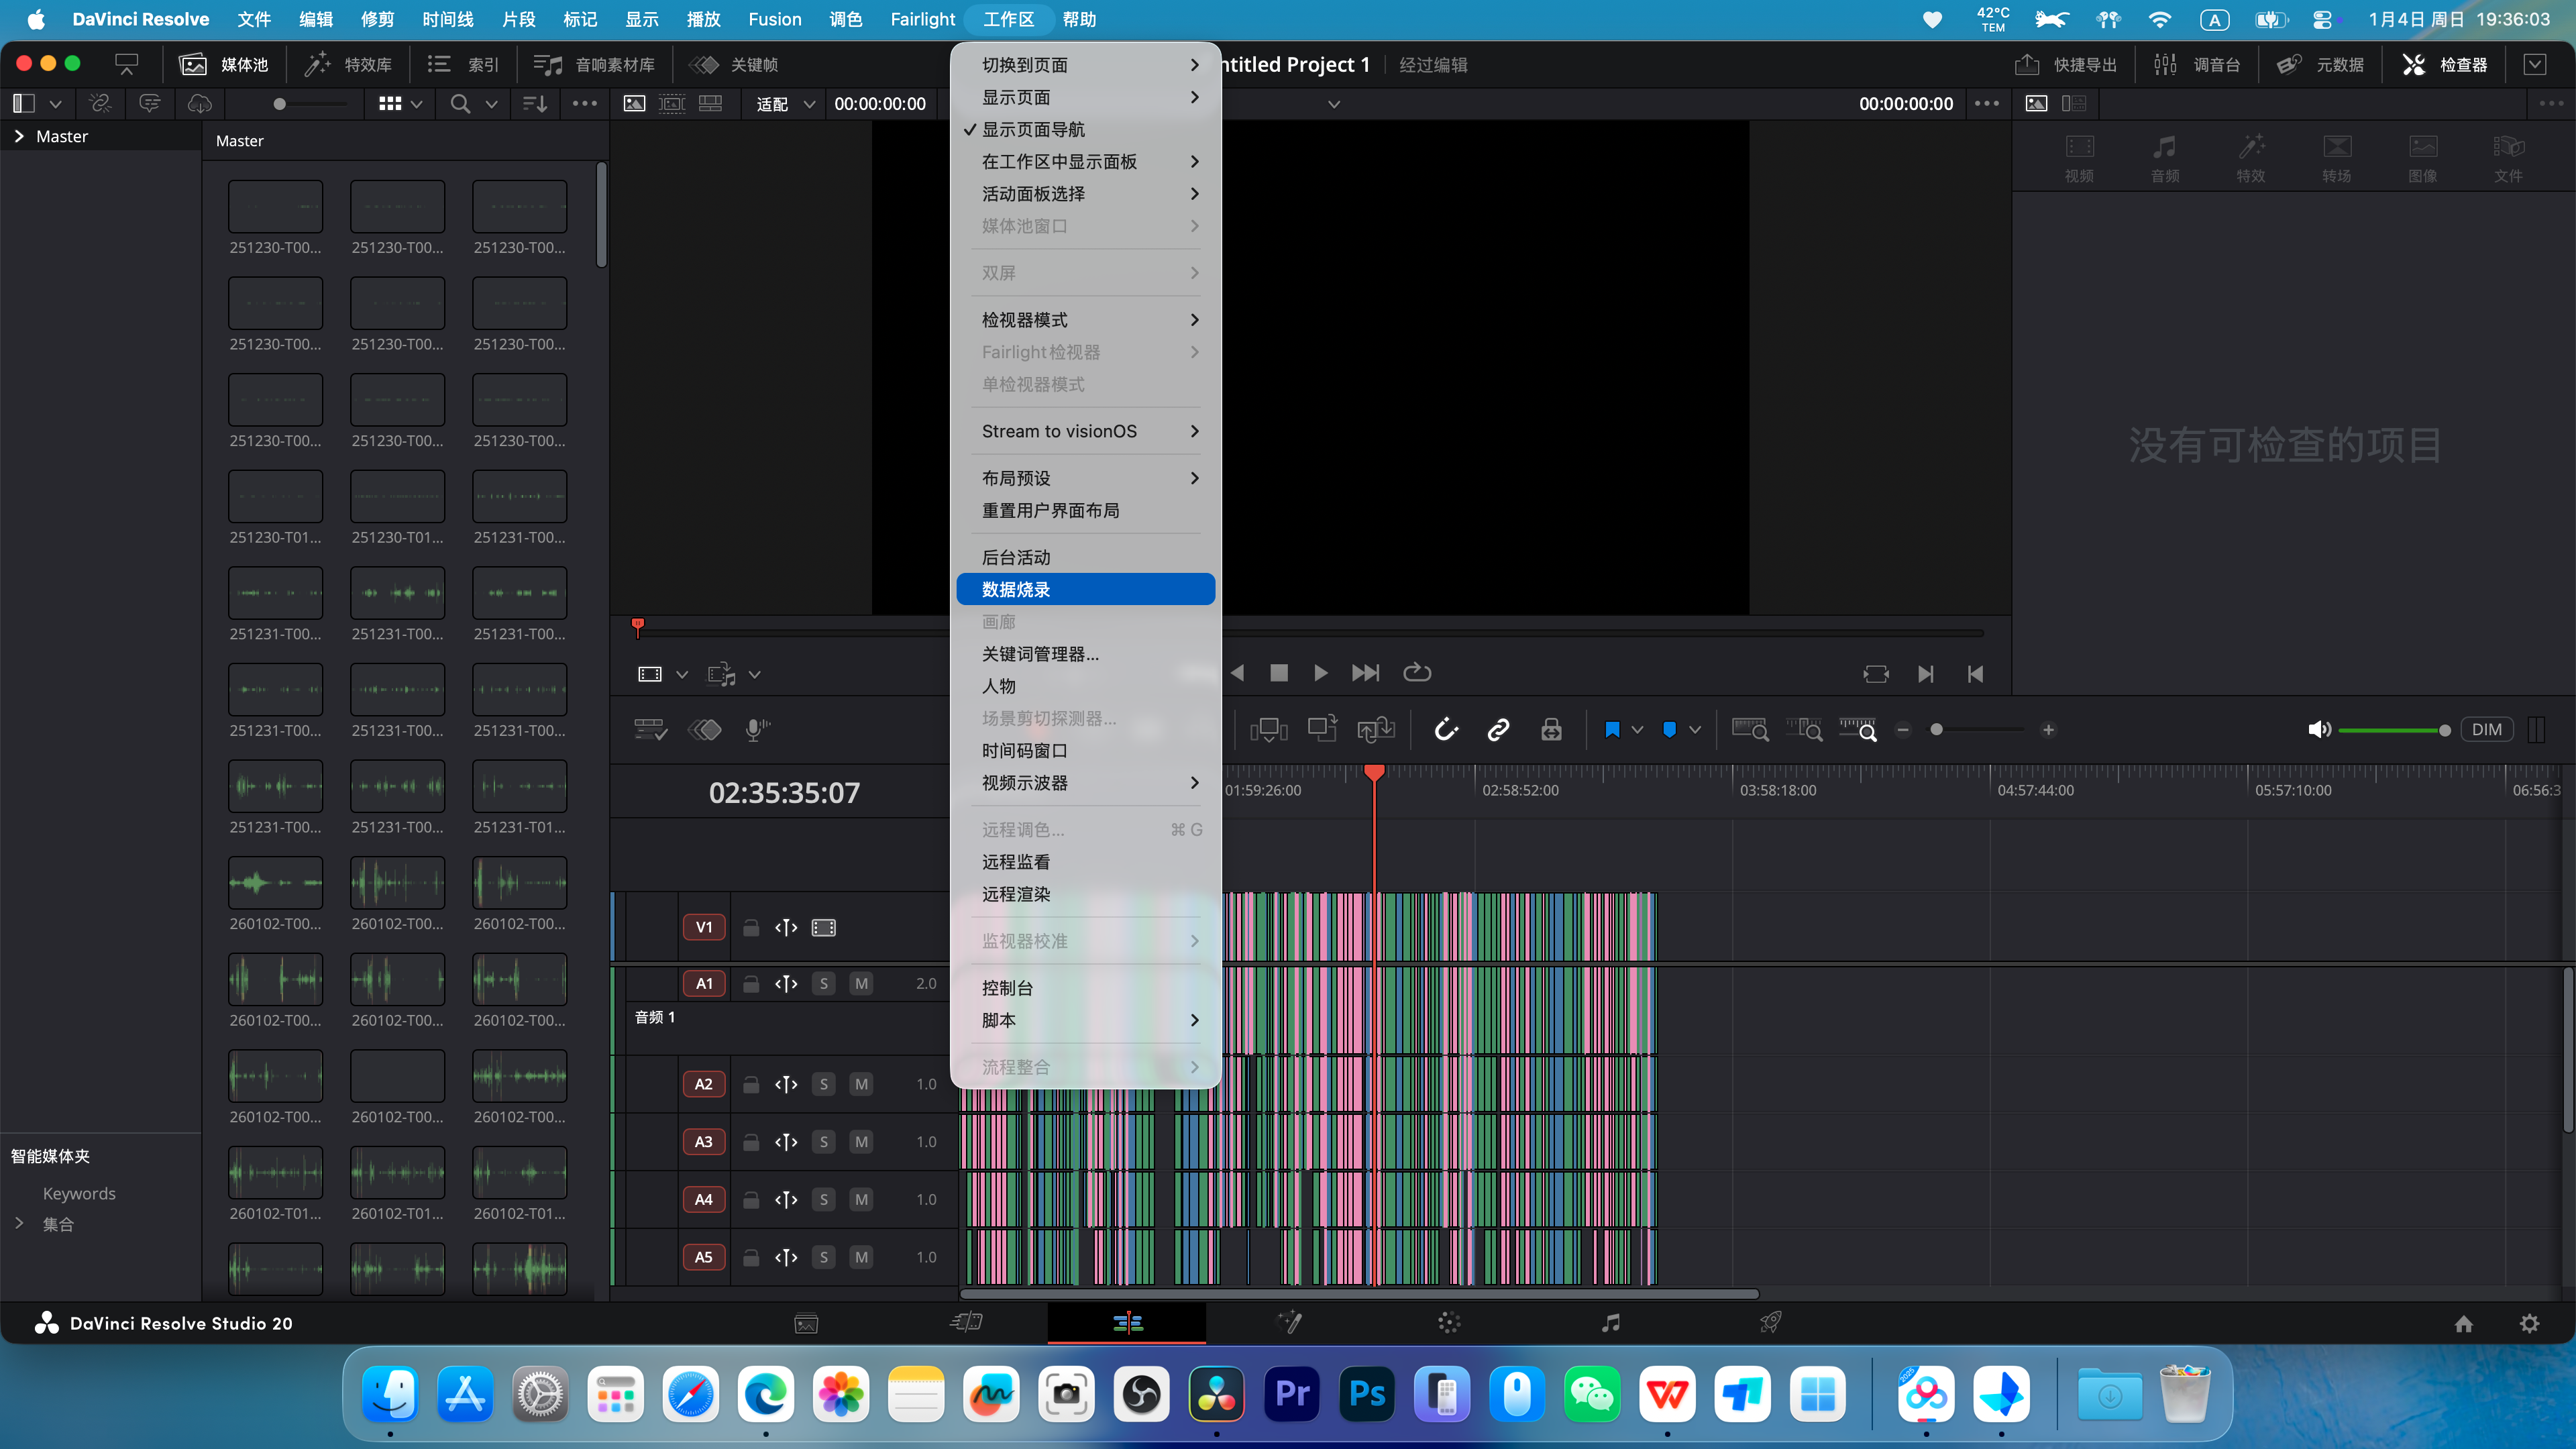
\includegraphics[width=\linewidth]{选择数据烧录.png} 
        \caption{在工作区菜单中开启数据烧录功能}
    \end{minipage}%
    \hfill%
    \begin{minipage}[t]{0.48\linewidth}
        \centering
        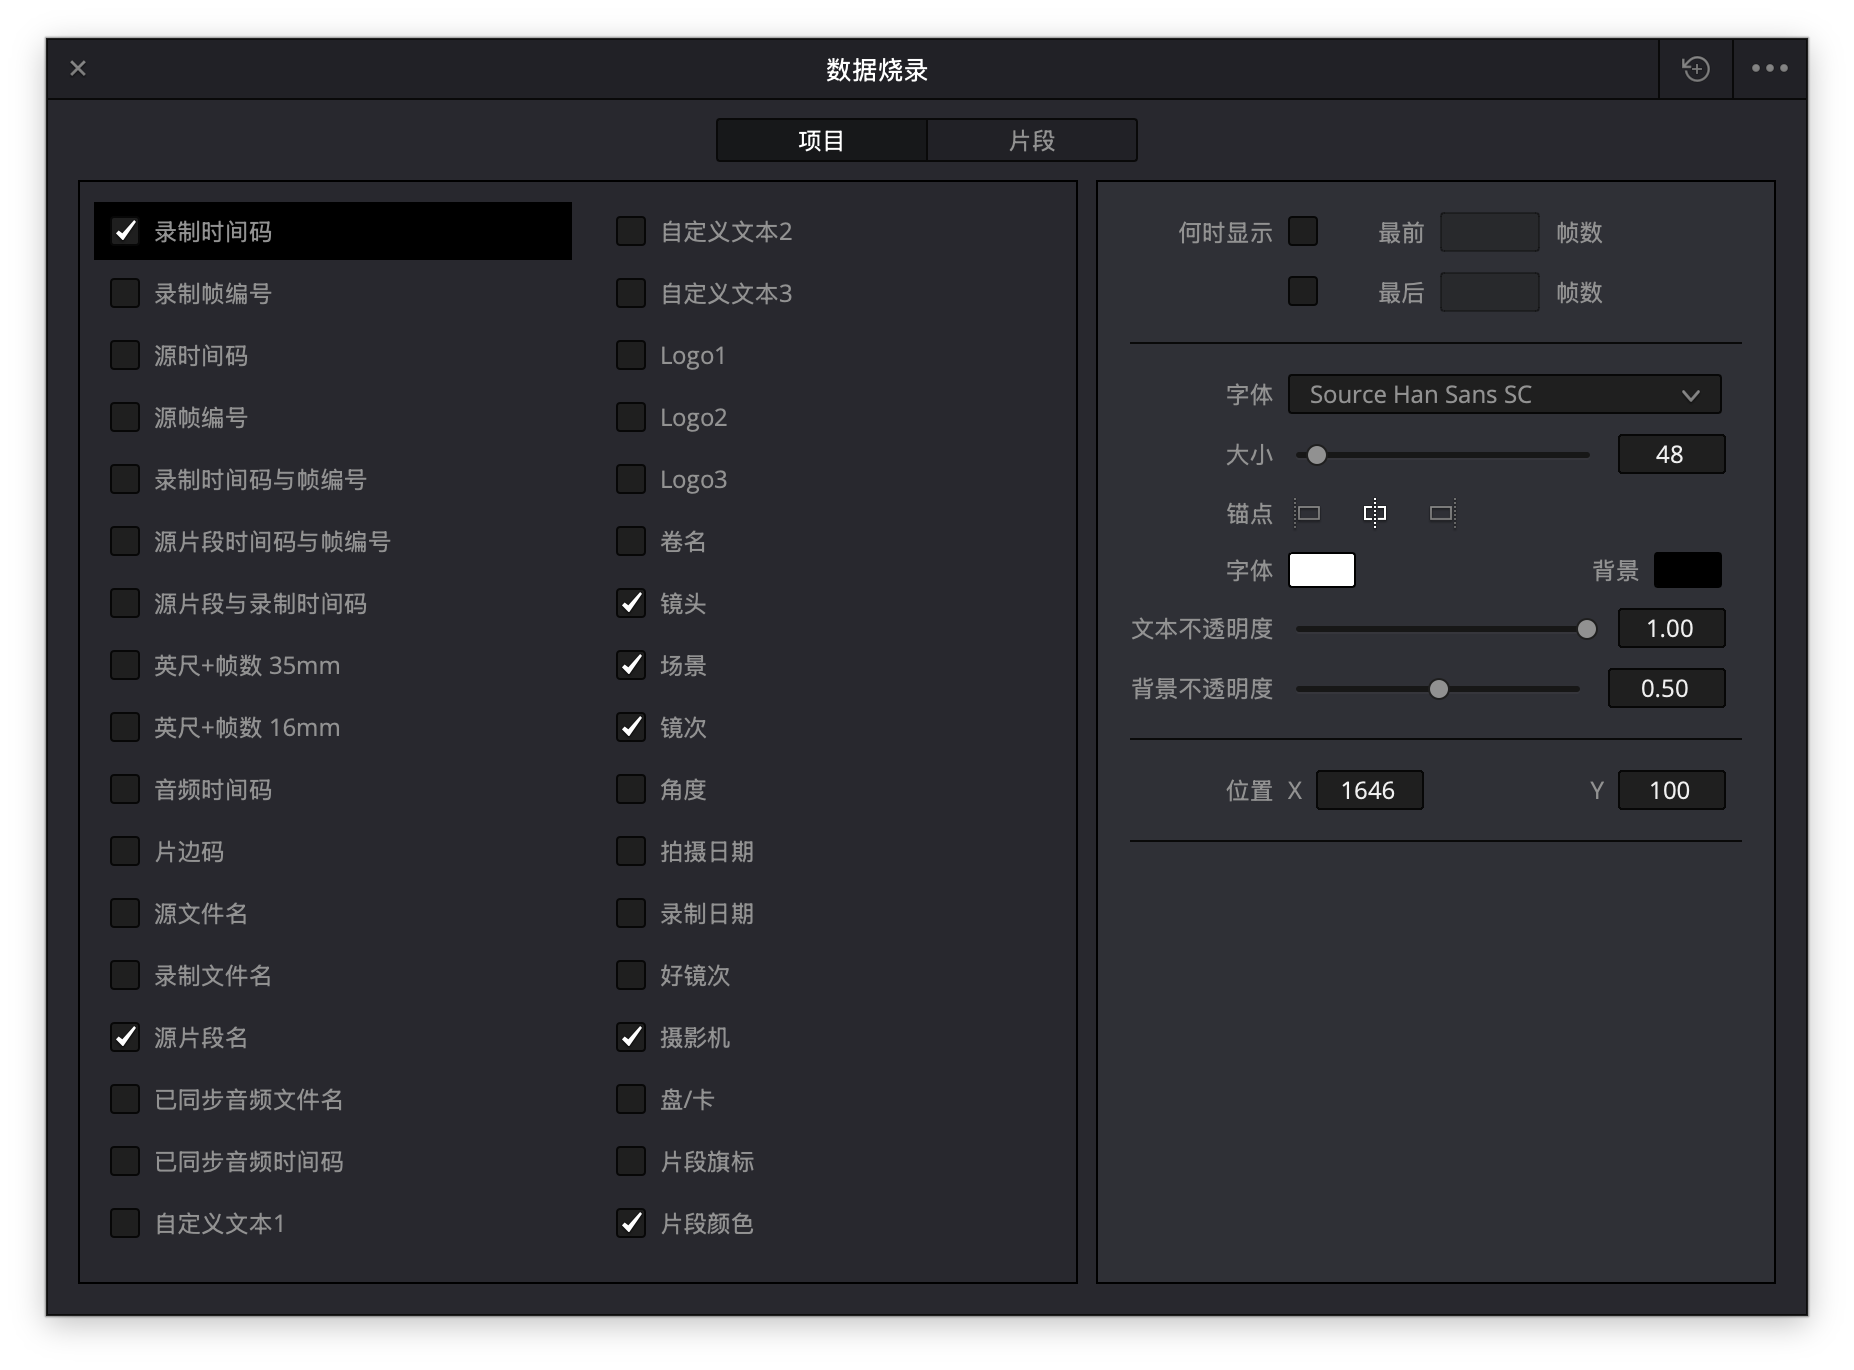
\includegraphics[width=\linewidth]{选择需要烧录的元数据.png} 
        \caption{勾选需要烧录的场记信息与时间码}
    \end{minipage}
\end{figure}

\textbf{步骤 5：导出交付媒体} \\
设置完成后，画面上就会实时显示出场记板信息。进入达芬奇的“交付”页面，在导出设置中，务必确保在“高级设置”里勾选了\textbf{“与项目相同的数据烧录”}，并选择\textbf{“单独片段”}进行导出。这样生成的 Proxy 文件就完美携带了所有的场记信息。
\begin{figure}[H]
    \centering
    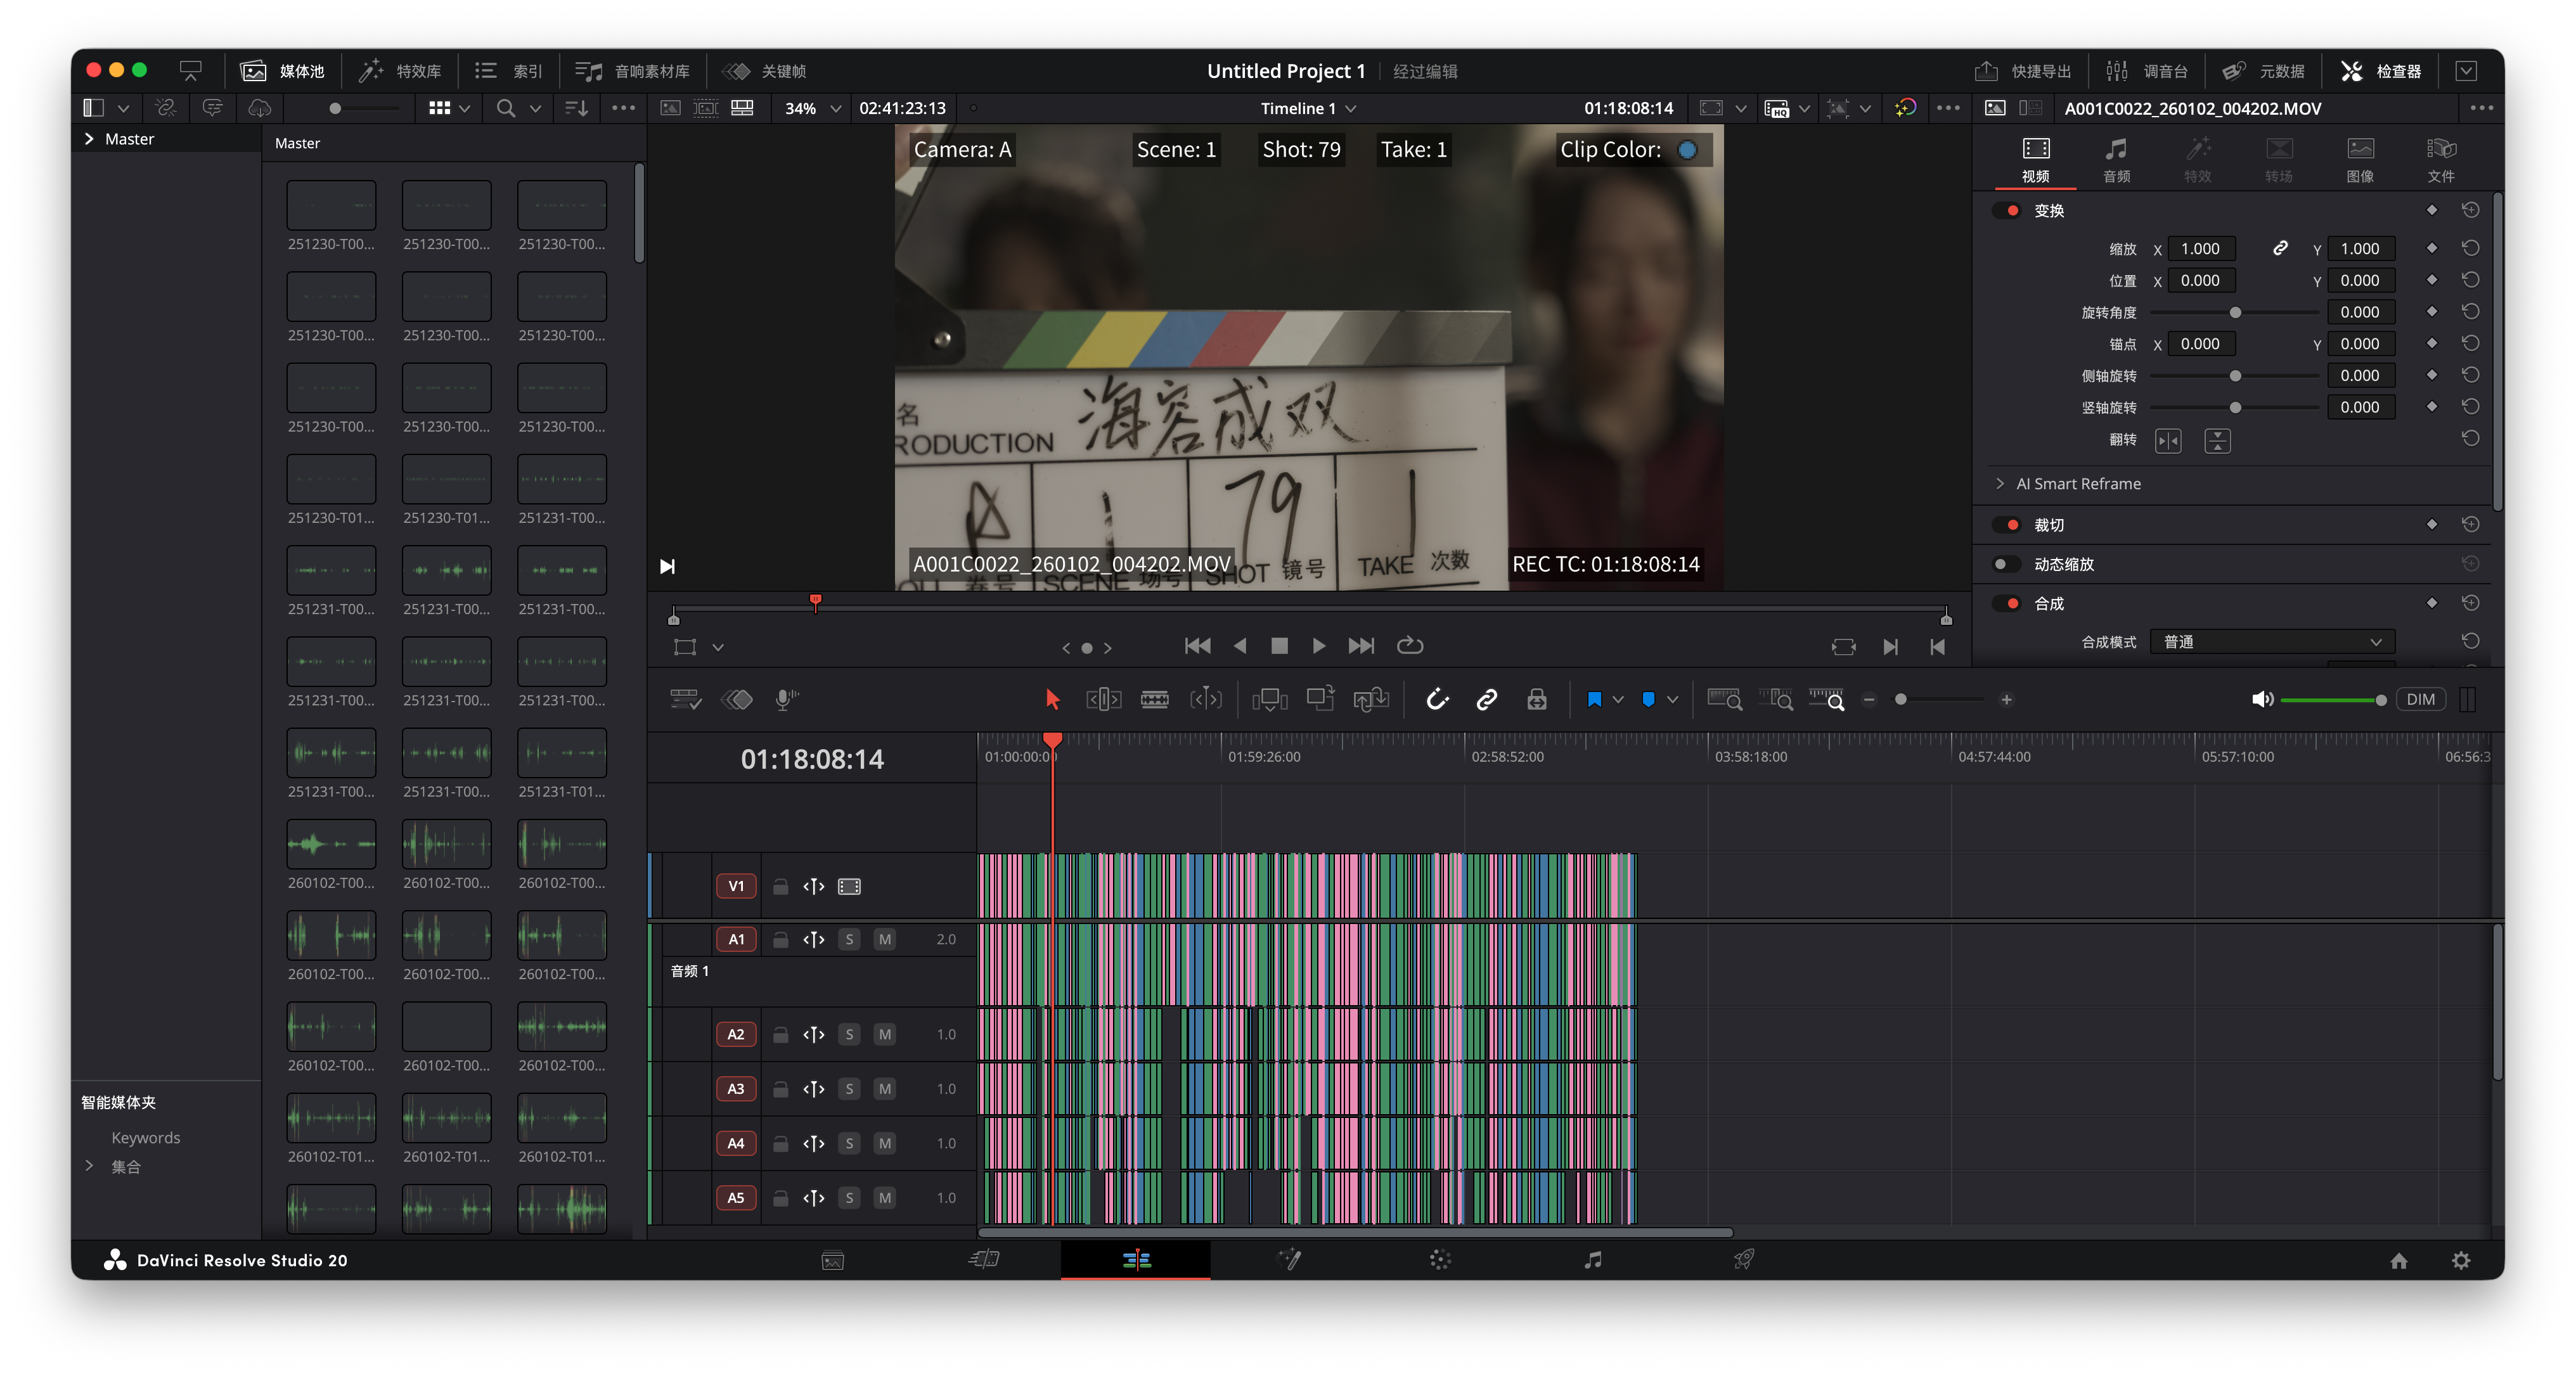
\includegraphics[width=0.95\linewidth]{可以看到达芬奇中出现了元数据，后续导出时在导出界面勾选数据烧录和单独片段导出即可.png} 
    \caption{画面出现烧录数据，准备导出单独的代理片段}
\end{figure}


\subsection{HDE (High Density Encoding) 拷贝、Codex 配置与恶性 Bug}

对于拍摄 ARRIRAW 的高级制作，为了大幅节省硬盘空间（通常可压缩至原大小的 60\%-70\%）且保持无损质量，我们通常会使用 HDE 技术进行素材的封装拷贝。但在最新的 macOS 环境下，Codex 的安装和权限配置往往会出现一些“卡脖子”的问题。

\textbf{问题一：drserver 权限报错} \\
在安装或运行 Codex 软件时，你可能会遇到以下提示导致进程卡死：

\begin{verbatim}
Codex Platform requires additional permissions. 
Click Open System Settings below and enable Full 
Disk Access for the Codex 'drserver' service.
\end{verbatim}

报错中提到的 \texttt{drserver} 是一个后台守护进程，它本身没有图形界面，所以不会自动出现在系统的“应用程序”列表中供你直接勾选。你需要通过手动指定路径将其添加到“完全磁盘访问权限”中。

\begin{tcolorbox}[colback=white, colframe=AlertRed, boxrule=1pt, arc=1mm, breakable, title={\textbf{解决 drserver 权限 Bug 的具体步骤}}]
\small
\textbf{第一步：打开系统设置}
\begin{itemize}
    \item 进入 \texttt{系统设置 (System Settings) -> 隐私与安全性 (Privacy \& Security) -> 完全磁盘访问权限 (Full Disk Access)}。
\end{itemize}

\textbf{第二步：点击添加与手动定位}
\begin{itemize}
    \item 点击列表下方的 \texttt{+} 号（添加按钮）。
    \item 当弹出一个 Finder 文件选择窗口时，\textbf{绝对不要}去手动点击文件夹寻找。
    \item 直接按下键盘快捷键：\texttt{Command + Shift + G}。
    \item 此时会弹出一个文本框，让你输入路径。准确输入：\\
          \texttt{/usr/local/codex/bin/drserver}
    \item 点击“前往”或按回车。
    \item 选中 \texttt{drserver} 文件并确认添加。虽然操作完后看起来好像什么都没有发生，但\textbf{重启电脑}之后，你会发现 Codex 服务已经成功启动。
\end{itemize}
\end{tcolorbox}

\textbf{如果你发现路径和我不一样：}
如果上述路径找不到文件，可以通过终端自己找：
\begin{enumerate}
    \item 打开 \texttt{终端 (Terminal)} app。
    \item 输入以下命令并回车，查找它的位置：\\
          \texttt{which drserver}
    \item 如果没找到，尝试全局搜索：\\
          \texttt{find /usr -name "drserver" 2>/dev/null}
    \item 终端会返回一个精确路径（例如 \texttt{/usr/sbin/drserver}）。
    \item 在 Finder 中，按下 \texttt{Command + Shift + G}，输入刚才找到的路径（\textbf{注意：去掉最后的 drserver 文件名，只进入所在的文件夹}）。
    \item 将文件夹里那个变成黑色终端样式的 \texttt{drserver} 图标，直接拖拽到“系统设置”的“完全磁盘访问权限”列表中即可。
\end{enumerate}

\vspace{0.3cm}
\begin{tcolorbox}[colback=white, colframe=AlertRed, boxrule=1pt, arc=1mm, breakable, title={\textcolor{WarningYellow}{\faExclamationTriangle} \textbf{严重警告：macOS 26 与 Silverstack 8.8.3 的 HDE 闪退 Bug}}]
\small
在最新的 \textbf{macOS 26} 系统下，8.8.3 学习版本的 Silverstack Lab 遇到 HDE 素材时会\textbf{百分之百触发闪退}。这是一个非常搞人心态的系统级恶性 Bug。

\textbf{现场临时救场工作流：}
\begin{enumerate}
    \item \textbf{“骗”过软件：} 先装载一次\textbf{非 HDE}的素材，正常写进元数据，建立好项目的基础结构。
    \item \textbf{使用 Offload 拷卡：} 遇到真正的 HDE 素材卡时，先关闭 Lab。改用 \textbf{Offload 试用版} 进行 HDE 文件的基础拷贝与校验。
    \item \textbf{补录元数据：} 基础拷贝完成后，再切回 Silverstack Lab 写入场记等相关元数据。
    \item \textbf{规避转码闪退：} 为了防止 Lab 在后续转码 Proxy 时碰到内部的 HDE 再次崩溃，你可以直接将卡里的原始素材转码出来，这样 Silverstack 库里就没有原生 HDE 文件了。
    \item \textbf{终极备用方案：} 如果现场赶时间（比如马上要换卡），请直接放弃在 Silverstack 中转码，无缝衔接使用本文 \ref{subsec:davinci_proxy} 节介绍的\textbf{“达芬奇出代理法”}来解决！
\end{enumerate}
\end{tcolorbox}


\subsection{进阶实战：开机前的摄影机宽容度与色彩测试}

作为全组最了解摄影机的人（确信），DIT 在开机前的测试（Camera Test）中扮演着至关重要的角色。这里以我们学校常用的 \textbf{RED Epic Dragon} 为例，展示在前期测试中，我们如何评估摄影机的核心光学素质。这些测试能帮你在现场给 DP 提供最准确的曝光建议，防止后期调色时“翻车”。

以下测试截图直观展示了由 RED Epic Dragon 拍摄（光源为两盏南光 f300）的素材，在经过套 LUT 和后期曝光拉回处理后的最终画面状态：

\begin{figure}[H]
    \centering
    \begin{minipage}[t]{0.31\linewidth}
        \centering
        \includegraphics[width=\linewidth]{暗部宽容度.png}
        \caption{暗部宽容度测试}
    \end{minipage}%
    \hfill%
    \begin{minipage}[t]{0.31\linewidth}
        \centering
        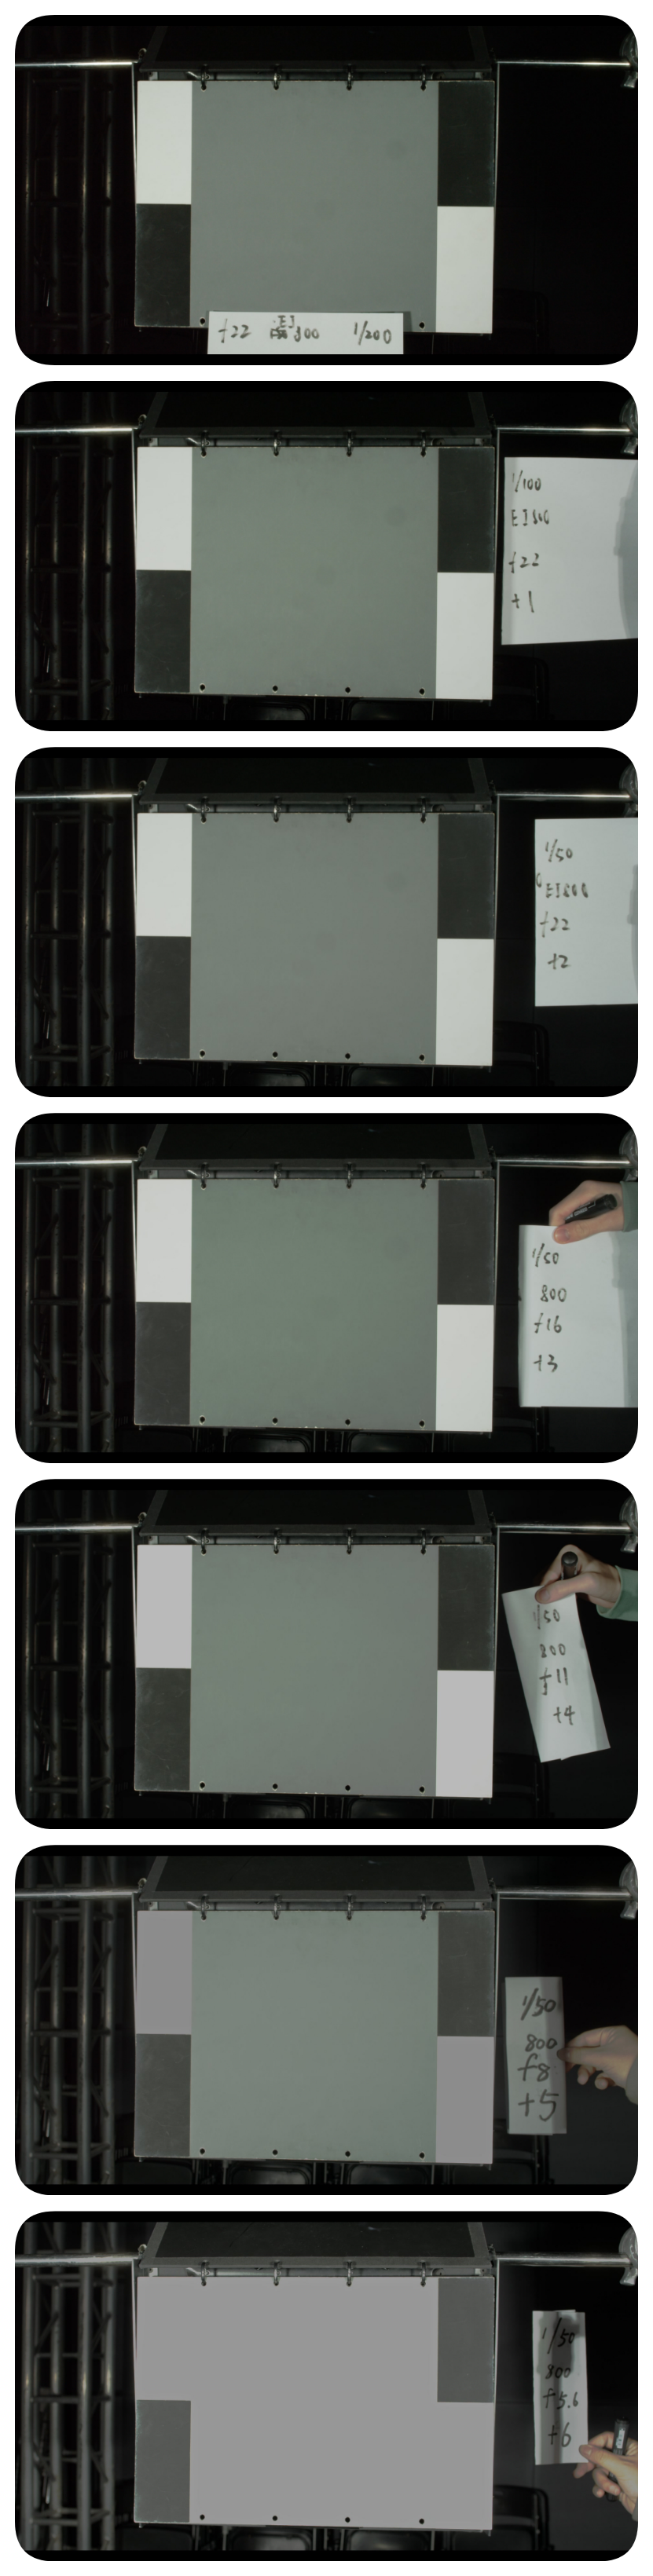
\includegraphics[width=\linewidth]{高光宽容度.png}
        \caption{高光宽容度测试}
    \end{minipage}%
    \hfill%
    \begin{minipage}[t]{0.31\linewidth}
        \centering
        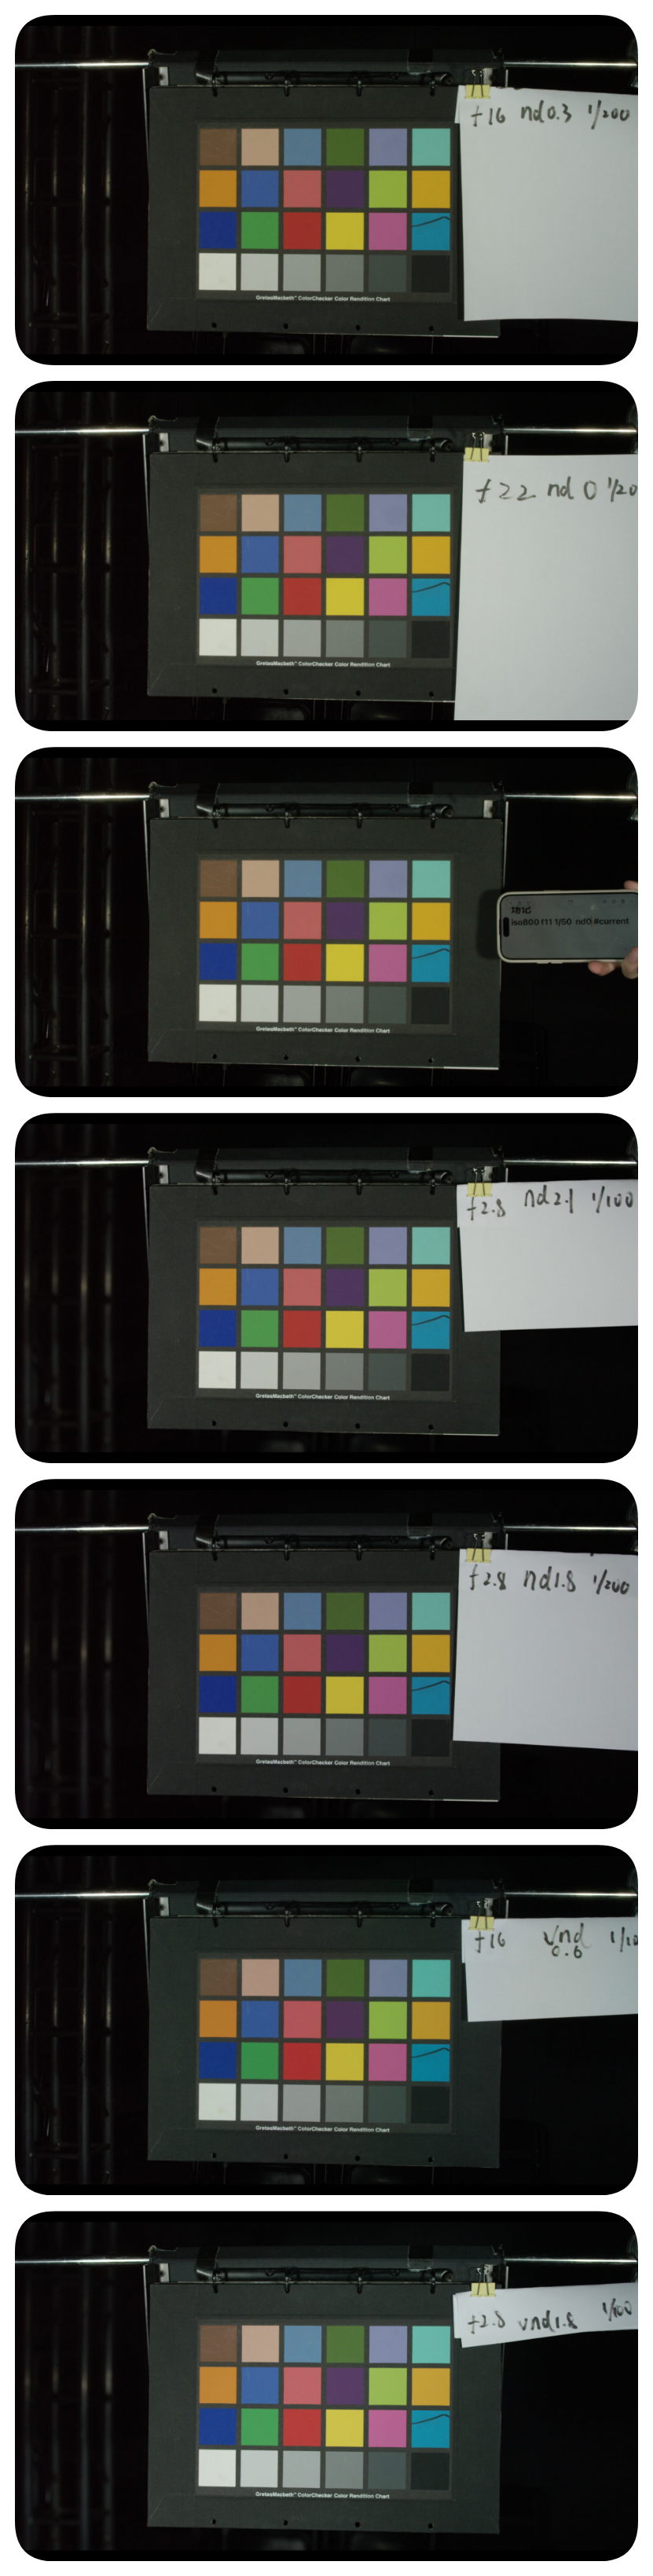
\includegraphics[width=\linewidth]{ND滤镜的色彩偏移（偏色）测试.png}
        \caption{ND 滤镜偏色测试}
    \end{minipage}
\end{figure}

\textbf{1. 暗部宽容度测试 (Under-exposure Latitude)}
\begin{itemize}
    \item \textbf{-1 到 -3 档：} 画面整体变暗，但 18\% 中性灰板和黑白块的边界依然清晰。在后期软件（如 DaVinci Resolve）中将其拉回到基准曝光后，通常能保持极高的画面可用性，信噪比（SNR）处于健康状态。
    \item \textbf{-4 到 -5 档：} 进入深度欠曝区域。画面信息虽然还在，但信号已经非常微弱。一旦在后期强行提亮，暗部会涌现出明显的噪点（尤其是彩色噪点 Chroma Noise）。
    \item \textcolor{AlertRed}{\textbf{-6 到 -8 档：}} 画面几乎完全被底噪（Noise Floor）淹没，尤其是 -7 和 -8，画面已经呈现出明显的品红色调偏移。这意味着传感器在这个光量下无法记录有效信息，即使勉强提亮，也会因为严重的色彩断层和固定模式噪点（FPN）而失去可用价值。
\end{itemize}

\textbf{2. 高光宽容度测试 (Over-exposure Latitude)}
\begin{itemize}
    \item \textbf{0 EV (基准)：} 快门 1/200，光圈 f/22。灰板、白块、黑块层次分明，曝光准确。
    \item \textbf{+1 到 +3 档：} 画面逐渐变亮，但白块依然保留了边缘和纹理，说明高光尚未溢出。在这个区间内，后期将曝光降回 0 EV，画面质感通常能完美还原。
    \item \textbf{+4 档：} 白块亮度逼近极限，开始有轻微的细节丢失趋势。
    \item \textcolor{AlertRed}{\textbf{+5 档 (高光溢出)：}} 左侧的纯白块已经完全“死白”（Clipping），和灰板之间的对比度大幅度压缩，高光信息开始发生实质性丢失。
    \item \textcolor{AlertRed}{\textbf{+6 档 (不可逆裁切)：}} 不仅白块完全溢出，18\% 灰板也即将过曝至死白，画面发灰。在这个档位，高光信息已经无法通过后期手段找回，出现了不可逆的裁切。
\end{itemize}

\textbf{3. ND 滤镜与色彩一致性测试 (ND Filter Color Shift Test)}
测试内容是在不同 ND 档位和光圈组合下，保持等效曝光，观察色卡（ColorChecker）的色彩偏移情况。
\begin{itemize}
    \item \textbf{基准状态 (ND 0.3 / ND 0)：} 这是极低浓度 ND 或无 ND 的状态，色彩还原最接近传感器的原生表现。
    \item \textbf{高浓度 ND 测试 (ND 1.8 / ND 2.1)：} 随着内置或外置 ND 浓度的增加，很多摄影机（尤其是早期的 RED 传感器）容易出现红外污染（IR Pollution）。仔细观察底部的中性灰阶，如果高浓度 ND 下的灰块偏向品红（Magenta）或棕红色，就说明滤镜产生了色偏。
    \item \textbf{VND (可调 ND) 测试 (VND 0.6 / VND 1.8)：} 可调 ND 由于是两片偏振镜叠加，更容易在特定角度产生不均匀的偏色或十字纹。对比固定 ND 滤镜的测试结果，可以明显评估这款 VND 的光学素质是否满足当前的工业要求。
\end{itemize}

\subsection{DIT 的保命黄金法则}

\begin{tcolorbox}[colback=white, colframe=AlertRed, boxrule=1pt, arc=1mm, title={\textbf{\faLock~ 来自李勃老师的绝对安全底线}}] 
\small
在片场，意外随时可能发生。请将 \libo{} 的以下核心原则刻在 DNA 里：
\begin{itemize}
    \item \textbf{素材安全大于一切：} \textbf{不应该给数据任何处在危险的机会中。}
    \item \textbf{给自己留一条后路：} 永远要想好最坏的情况发生了该怎么办。
    \item \textbf{不要说“应该”：} 数据在就是在，不在就是不在。\textbf{要用工作流程和制度确保安全}，而不是依靠技术玄学和人员能力。
    \item \textbf{Double Check：} 永远保持怀疑，永远交叉验证。
\end{itemize}
\end{tcolorbox}
\vspace{0.3cm}

基于以上底线原则，在现场必须严格遵守以下具体操作规范：
\begin{itemize}
    \item \textbf{3-2-1 原则：} 至少要有 3 份数据，即1张原卡加2块硬盘；存放在 2 种不同的介质上；其中 1 份最好在异地，例如百度网盘。
    \item \textbf{红绿胶带法：}
    \begin{itemize}
        \item \textcolor{AlertRed}{\textbf{红胶带封住读卡器或卡盒}}：代表未备份，危险！
        \item \textcolor{SafeGreen}{\textbf{绿胶带封住卡盒}}：代表已备份，安全，可以格式化。
    \end{itemize}
    \item \textbf{永远不要自己格式化卡！} 即使备份好了，也要把绿胶带封好的卡交还给摄影助理，让他们上机确认后自己操作。
    \item \textbf{不要相信 Finder：} 永远不要用鼠标直接把文件从卡里拖到硬盘里！如果必须这么做，例如软件挂了，请使用免费软件 DaVinci Resolve 的克隆工具功能，它同样带有校验保护。
    \item \textbf{眼见为实：} 机器显示“校验成功”后，必须随机打开几个视频文件，尤其是每张卡的最后一条，拖动一下进度条看看有没有问题。
    \item \textbf{不接电，不干活：} 拷卡过程非常耗电，如果中途断电导致硬盘掉线，可能会损坏文件系统。务必确保 Mac 和硬盘都在稳定供电状态。
\end{itemize}
% ------------------------------------------
% 结尾/致谢页 
% ------------------------------------------
\newpage
\thispagestyle{empty} % 清除这一页的页眉页脚
\begin{tcolorbox}[
    colback=LightBlue, 
    colframe=DITBlue, 
    boxrule=1pt, 
    arc=2mm, 
    left=5mm, right=5mm, top=3mm, bottom=3mm, 
    before upper=\setlength{\parindent}{2em} 
]

    \phantomsection 
    \addcontentsline{toc}{section}{结语 （附图《正在激情授课的李勃老师》）} 
    \begin{center}
        {\Large \textbf{\textcolor{DITBlue}{结语：守住底线，捍卫尊严}}}
    \end{center}
    
    \vspace{-0.2cm} 
    
    这只是一份面向零基础新手的快速入门教程。加上出于某些不可抗力（主要是我比较懒），内容肯定有许多不周到、不严谨的地方，还请大家谅解。如果你在实战中发现了错漏，或者有更好的建议，欢迎随时联系我，我会进行修改和完善。
    
    最后，无论你身处多大多小的剧组，请务必维护好 DIT 这个岗位的尊严——做一个极其靠谱的人，绝不能给这个职位丢脸，更\textbf{绝对不能丢数据}。请收起你不合时宜的好奇心，\textbf{千万不要在正式开机的剧组里去尝试任何未经测试的“新流程”}，按部就班、稳妥行事才是王道。正如 \libo{} 曾经反复教诲的那样：\textbf{“没有标准就没有技术流程。”}相信有一天作者也能在未来将标准的流程用到标准的工业拍摄流程中去！
    
    在此，特别感谢 \libo{} 的悉心教导与专业指引，感谢 \xuchenyi{} 给予的帮助，感谢 \linchengyang{} 在软件和技术问题上提供的有力支持，以及所有在实践中给予我帮助的 23 级同学们。
    
    \vspace{0.1cm}
    
    \begin{center}
        \includegraphics[width=0.35\linewidth]{libo_ai.png}
        
        \vspace{0.1cm}
        \small\textcolor{TextGrey}{\textbf{图：}史料记载中正在激情授课的李勃老师}
    \end{center}
    
    \vspace{0.01cm}
    \noindent\rule{\linewidth}{0.5pt} 
    \vspace{0.1cm}
    
    {\raggedleft \small
    \textbf{当前版本：} V1.1 \\
    ZQ \\
    189 1157 0407 \\
    北京电影学院 智能影像工程学院 \par}
\end{tcolorbox}
\end{document}